\documentclass[reqno]{amsart}
\usepackage[T1]{fontenc}
\usepackage{lmodern} % Use this instead of courier/beramono
\usepackage[inner=1.0in,outer=1.0in,bottom=1.0in, top=1.0in]{geometry}
\usepackage[utf8]{inputenc}
\usepackage{amsfonts}
\usepackage{amsmath}
\usepackage{amssymb}
\usepackage{amsthm}
\usepackage{hyperref}
\usepackage{ dsfont }
\usepackage{cleveref}
\usepackage{ gensymb }
\usepackage{tikz}
\usetikzlibrary{calc, quotes, angles}
\usepackage{tikz-cd}
\usepackage{graphicx}
\usepackage{verbatim}
\usepackage{soul}
\usepackage{pgfplots}
\usepackage{textcomp}
\pgfplotsset{compat=newest}
\usepgfplotslibrary{fillbetween}

\usepackage{inconsolata}
\usepackage{xcolor}
\usepackage{listings}

\definecolor{codegreen}{rgb}{0,0.6,0}
\definecolor{codegray}{rgb}{0.5,0.5,0.5}
\definecolor{codepurple}{rgb}{0.58,0,0.82}
\definecolor{backcolour}{rgb}{0.96,0.96,0.96}
\definecolor{agblue}{rgb}{0.08,0.22,0.38}
\definecolor{aggreen}{rgb}{0.05,0.32,0.22}
\definecolor{agcodebg}{rgb}{0.92,0.96,1.0}

\lstdefinestyle{shellstyle}{
    basicstyle=\ttfamily\small,
    breaklines=true,
    showstringspaces=false,
    backgroundcolor=\color{backcolour},
}

\lstdefinestyle{pythonstyle}{
    language=Python,
    basicstyle=\ttfamily\small,
    keywordstyle=\color{blue},
    commentstyle=\color{codegray}\itshape,
    stringstyle=\color{codepurple},
    showstringspaces=false,
    breaklines=true,
    numbers=left,
    numberstyle=\tiny\color{codegray},
    backgroundcolor=\color{backcolour},
    frame=single,
}

\lstset{style=shellstyle}

\newenvironment{lecturebox}[1]{%
    \par\medskip
    \noindent\begingroup
    \setlength{\parindent}{0pt}
    \color{agblue}\hrule height 0.8pt\color{black}
    \smallskip
    \textbf{\color{agblue}#1}\par\smallskip
}{%
    \smallskip
    \color{agblue}\hrule height 0.8pt\color{black}
    \endgroup
    \medskip
}

\newcommand{\keyterm}[1]{\textbf{\color{agblue}#1}}
\newcommand{\examplepart}[1]{%
    \par\medskip
    \noindent\textbf{\color{agblue}#1}\par\smallskip\noindent
}
\newcommand{\codeseg}[1]{%
    \begingroup
    \setlength{\fboxsep}{1.5pt}%
    \colorbox{agcodebg}{\texttt{\detokenize{#1}}}%
    \endgroup
}

\DeclareMathOperator{\inv}{^{-1}}
\DeclareMathOperator{\stab}{stab}
\DeclareMathOperator{\Ocal}{\mathcal{O}}
\DeclareMathOperator{\ord}{ord}
\DeclareMathOperator{\graph}{graph}
\DeclareMathOperator{\fix}{fix}
\DeclareMathOperator{\rr}{\mathbb{R}}
\DeclareMathOperator{\cc}{\mathbb{C}}
\DeclareMathOperator{\nn}{\mathbb{N}}
\DeclareMathOperator{\zz}{\mathbb{Z}}
\DeclareMathOperator{\qq}{\mathbb{Q}}
\DeclareMathOperator{\Aut}{Aut}
\DeclareMathOperator{\Sym}{Sym}
\DeclareMathOperator{\id}{id}
\DeclareMathOperator{\lcm}{lcm}
\DeclareMathOperator{\Syl}{Syl}
\DeclareMathOperator{\sgn}{sgn}
\DeclareMathOperator{\Acal}{\mathcal{A}}
\DeclareMathOperator{\Ob}{Ob}
\DeclareMathOperator{\Hom}{Hom}
\DeclareMathOperator{\Cat}{Cat}
\DeclareMathOperator{\Isom}{Isom}
\DeclareMathOperator{\coker}{coker}
\DeclareMathOperator{\im}{im}
\DeclareMathOperator{\ff}{\mathbb{F}}
\renewcommand{\aa}{\mathbb{A}}
\DeclareMathOperator{\pp}{\mathbb{P}}
\DeclareMathOperator{\rank}{rank}
\DeclareMathOperator{\Lcal}{\mathcal{L}}
\DeclareMathOperator{\Div}{Div}
\DeclareMathOperator{\genus}{genus}
\DeclareMathOperator{\Nred}{N_{red}}
\DeclareMathOperator{\Pic}{Pic}
\DeclareMathOperator{\tors}{tors}
\DeclareMathOperator{\End}{End}
\renewcommand{\div}{\text{div}}
\DeclareMathOperator{\Mcal}{\mathcal{M}}
\DeclareMathOperator{\GL}{GL}
\DeclareMathOperator{\cont}{Content}
\DeclareMathOperator{\afrak}{\mathfrak{a}}
\DeclareMathOperator{\bfrak}{\mathfrak{b}}
\DeclareMathOperator{\cfrak}{\mathfrak{c}}
\DeclareMathOperator{\ofrak}{\mathfrak{o}}
\DeclareMathOperator{\hfrak}{\mathfrak{h}}
\DeclareMathOperator{\mfrak}{\mathfrak{m}}
\DeclareMathOperator{\nfrak}{\mathfrak{n}}
\DeclareMathOperator{\pfrak}{\mathfrak{p}}
\DeclareMathOperator{\qfrak}{\mathfrak{q}}
\DeclareMathOperator{\Dcal}{\mathcal{D}}
\DeclareMathOperator{\Res}{Res}
\DeclareMathOperator{\dist}{dist}
\DeclareMathOperator{\vvert}{\vert \vert}
\DeclareMathOperator{\Ccal}{\mathcal{C}}
\DeclareMathOperator{\Area}{Area}
\DeclareMathOperator{\Volume}{Volume}
\DeclareMathOperator{\Bfrak}{\mathfrak{B}}
\DeclareMathOperator{\Gal}{Gal}
\DeclareMathOperator{\li}{li}
\DeclareMathOperator{\re}{Re}
\DeclareMathOperator{\supp}{supp}
\DeclareMathOperator{\Afrak}{\mathfrak{A}}
\DeclareMathOperator{\tpi}{\frac{1}{2\pi i}}
\DeclareMathOperator{\SL}{SL}
\DeclareMathOperator{\PSL}{PSL}
\DeclareMathOperator{\SO}{SO}
\DeclareMathOperator{\hh}{\mathbb{H}}
\DeclareMathOperator{\Fcal}{\mathcal{F}}
\DeclareMathOperator{\Hcal}{\mathcal{H}}
\DeclareMathOperator{\tr}{Trace}
\DeclareMathOperator{\Tcal}{\mathcal{T}}
\DeclareMathOperator{\1}{\textbf{1}}
\DeclareMathOperator{\ad}{ad}
\DeclareMathOperator{\asai}{asai}
\DeclareMathOperator{\sym}{sym}
\DeclareMathOperator{\res}{res}
\DeclareMathOperator{\PGL}{PGL}
\DeclareMathOperator{\qterm}{(1+\vert D\vert^{3/2})}
\newcommand{\Mod}[1]{\ (\mathrm{mod}\ #1)}
\newcommand{\norm}[1]{\left\lVert#1\right\rVert}

\newtheorem{thm}{Theorem}[section]
\newtheorem{prop}[thm]{Proposition}
\newtheorem{lemma}[thm]{Lemma}
\newtheorem{example}[thm]{Example}
\newtheorem{cor}[thm]{Corollary}
\newtheorem{defn}[thm]{Definition}
\newtheorem{remark}[thm]{Remark}
\newtheorem{conj}[thm]{Conjecture}
\DeclareMathOperator{\xx}{\mathbb{X}}
\newcommand{\psum}{\sideset{}{'}\sum}
\newcommand{\hashsum}{\mathop{\sum}\limits^{\#}}
\newcommand{\tmod}[1]{\ \left(\text{mod }#1\right)}


\title{Euclidean Geometry and AI}
\author{Steven Creech}
\address{Department of Mathematics \\ Brown University \\ Providence, RI 02906
\\ USA}
\email{steven\_creech@brown.edu}

\author{Peter Zenz}
\address{Department of Mathematics \\ Brown University \\ Providence, RI 02906
\\ USA}
\email{peter\_zenz@brown.edu}
\date{\today}

\begin{document}
\begin{abstract}
    The following document consists of lecture notes that came out of a special
    topics course at Brown University in Fall of 2025 on Euclidean Geometry and
    Artificial Intelligence. The hope is that this document is created in such a
    way that others can replicate this course at their own universities. In
    addition to this document, there is an accompanying github repository where
    there are coded outlines for homeworks with corresponding tests for the
    code.
\end{abstract}
\maketitle
\tableofcontents

\newpage

Completion of the writing:

\begin{enumerate}
    \item  
    \item 
    \item Arichitecture of Our System 
    \item 
    \item Basic Geometric Objects 
    \item Basic Predicates 
    \item Problem Data Structure
    \item Deductive Database
    \item Generating Conjectures
    \item Algebraic Reasoning
    \item Implementing Area
    \item Auxliary Constructions
    \item Generating Synthetic Data
    \item Cleaning the Data
    \item 
    \item 
    \item 
    \item 
    \item 
    \item
    \item 
    \item 
    \item 
    \item 
    \item 
    \item 
    \item Homework
\end{enumerate}

\newpage

\section{Introduction}\label{sec: Intro}
There are two aspects to this course: learning geometry in a broad sense and
building an AI that can solve Euclidean geometry problems. In terms of geometry,
the topics covered include: powers of points, radical axis, Ceva's theorem,
Menelaus's theorem, Pappuss's Hexagon theorem, Pascal's theorem, and Brianchon's
theorem. After talking about these more classical results of Euclidean geometry.
The course then turned to Hilbert's axiomization of geometry \cite{hartshorne2013geometry}.


As for the coding aspect of the course, in building the AI the topics covered
include: formalizing geometry problems, neuro-symbolic reasoning, generating
random diagrams, creating synthetic data, cleaning data, $n$-shot prompting and fine-tuning language models. We also include a few references to automatic diagram generation and auto-formalization, but we do not go into these topics, the ambitious students may attempt to incorporate these ideas into their systems. 

By the end of the course, students will have created an AI that is akin to that
of Google Deepminds AlphaGeometry  \cite{chervonyi2025gold}.


The course was structured in a way that there are 3 lectures in a week. 2
lectures are about geometry, and then there is a lecture about implementing and
building the AI. These two concepts go hand in hand, but the main focus of these notes are on the implementation. At the beginning of the semester some of the mathematical lectures
were used to discuss formal language, and conventions used. This document is
more concerned with the implementation of the AI; thus, the beginning focus on the mathematics is more concerned with setting up a uniform notation for the AI systems. At the end of these notes, we also include several of the more classical theorems of Euclidean geometry discussed in the course with some discussion on caveats if these were to be implemented into our systems. 

During the original offering of the course, we left the coding aspect open
ended. This was good in that some students came up with some great ideas in
their implementations; however, it also led to students having several issues
with bugs in their work. Thus, in this document, we give a more structured
outline of the coding that comes from some of the ideas of the students.
However, we encourage any students following through this document and building
their own system if they have any optimizations or additions they should add
them. By doing this, we hope that in future courses, students will have a
combination of both structure and freedom in creating their AI.

\textbf{A Statement on AI Usage:} In the initial run of this course, we encouraged students to use AI to aid them in the creation of their systems. Furthermore, in the creation of these notes, AI was used in helping of the creation of diagrams and synthesizing the prose, and creating code outlines and tests for homework. Everything that was generated by an AI was looked over by a human, and we expect that students to also go over all artifacts created by AI. 

\section{AlphaGeometry Overview}
The following notes contains a high level overview of how the AlphaGeometry
system works.

\noindent \textbf{What is AlphaGeometry:} It is a neuro-symbolic reasoning
system to solve Euclidean geometry problems. The \textbf{symbolic reasoning}
corresponds to using formal logic and rule based reasoning. This is good because
by combining theorems using logical rigor will guarantee the correctness of the
solution. The \textbf{neuro network} corresponds to using pattern recognition
and learning from a large set of data to solve the problem. In principal, if
prompting a LM with a geometry problem there is no guarantee that the solution
is correct and that the LM did not hallucinate. Thus, the power of AlphaGeometry
comes in combining the two strategies. We use the \textbf{neuro} aspect to come
up with ideas, and then we use the \textbf{symbolic} aspect to give precise
reasoning and insure that the solution is correct.

There are three main components to AlphaGeometry:
\begin{enumerate}
    \item DD (deductive database)
    \item AR (algebraic reasoning)
    \item LM (language model)
\end{enumerate}
DD and AR correspond to the \textbf{symbolic} aspect of the system, and the LM
corresponds to the \textbf{neuro} aspect. In particular, DD corresponds to a
list of rules/theorems that combine different statements to deduce new
statements. AR then uses linear algebra to speed up the reasoning done with DD.
The general idea is to use DDAR to solve the problem; however, if the problem
cannot be solved by DDAR, then the LM is prompted and asked to give an auxiliary
construction. Then the hope is that with this auxiliary construction, then DDAR
can solve the problem. We shall call these auxiliary constructions
\textbf{rabbits} as a magician pulls a rabbit out of a hat when we are given
this magical rabbit, then the symbolic system of DDAR can solve the problem.

The LM knows which rabbits to give since it will be trained on theorems and
proofs. Thus, by looking at patterns in proofs it has been trained on, the LM
will suggest rabbits that are useful in solving the given problem.

\begin{example}
    Let $ABC$ be any triangle with $AB = AC$. Prove that $\angle ABC = \angle
    ACB$.

    In order to prove this, we must first give the computer a formalized version
    of this natural language problem. Such as
    \begin{itemize}
        \item \verb|[1] ncol A B C| (this will say that the points $A,B,C$ are not collinear that is that they form a triangle)
        \item \verb|[2] cong A B A C| (this will say that the segment $AB$ is congruent to the segment $AC$)
        \item \verb|[?] eqangle A B C A C B| (this is saying that we are asking if the angle $ABC$ is equal to the angle $ACB$)
    \end{itemize}
    We must also supply the computer with a diagram of the problem (Google
    Deepmind's AlphaGeometry has an autoformalizer and auto diagram generator;
    however, in this course we will supply the computer with both of these).
    \begin{center}
\begin{tikzpicture}[scale=2, line cap=round]
    \usetikzlibrary{calc}

    % Coordinates
    \coordinate (A) at (0,1.6);
    \coordinate (B) at (-1,0);
    \coordinate (C) at (1,0);

    % Triangle
    \draw (A) -- (B) -- (C) -- cycle;

    % ---- Tick mark on AB ----
    \path let \p1 = ($(B)-(A)$) in
        coordinate (Mab) at ($(A)!0.5!(B)$)
        coordinate (PerpAB1) at ($(Mab)!0.08! 90:(B)$)
        coordinate (PerpAB2) at ($(Mab)!0.08!270:(B)$);
    \draw (PerpAB1) -- (PerpAB2);

    % ---- Tick mark on AC ----
    \path let \p1 = ($(C)-(A)$) in
        coordinate (Mac) at ($(A)!0.5!(C)$)
        coordinate (PerpAC1) at ($(Mac)!0.08! 90:(C)$)
        coordinate (PerpAC2) at ($(Mac)!0.08!270:(C)$);
    \draw (PerpAC1) -- (PerpAC2);

    % Labels
    \node[above] at (A) {$A$};
    \node[left]  at (B) {$B$};
    \node[right] at (C) {$C$};
\end{tikzpicture}
\end{center}
While this problem in principle is just saying that in an isosceles triangle the two angles opposite of the two sides of the same length are the same. This could be considered as a rule in DD, in which we could just apply the rule to conclude the theorem. However, let us say that we have a smaller DD in which we only know SSS congruence of triangles. Then as written we cannot solve the problem; thus, we might prompt the LM. Say that the LM suggests the following construction: Let $D$ be the midpoint of $BC$ (i.e. \verb|midp D B C|). Then the picture becomes 

\begin{center}
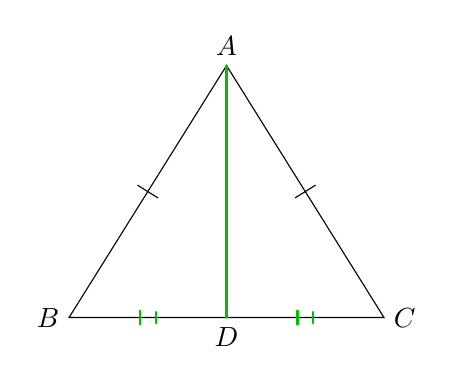
\begin{tikzpicture}[scale=2, line cap=round]
\usetikzlibrary{calc}
% Coordinates
\coordinate (A) at (0,1.6);
\coordinate (B) at (-1,0);
\coordinate (C) at (1,0);
\coordinate (D) at (0,0);  % midpoint of BC
% Triangle
\draw (A) -- (B) -- (C) -- cycle;
% Segment AD (dark green)
\draw[green!75!black, thick] (A) -- (D);
% ---- Tick marks on AB (single) ----
\path let \p1 = ($(B)-(A)$) in
    coordinate (Mab) at ($(A)!0.5!(B)$)
    coordinate (PerpAB1) at ($(Mab)!0.08! 90:(B)$)
    coordinate (PerpAB2) at ($(Mab)!0.08!270:(B)$);
\draw (PerpAB1) -- (PerpAB2);
% ---- Tick marks on AC (single) ----
\path let \p1 = ($(C)-(A)$) in
    coordinate (Mac) at ($(A)!0.5!(C)$)
    coordinate (PerpAC1) at ($(Mac)!0.08! 90:(C)$)
    coordinate (PerpAC2) at ($(Mac)!0.08!270:(C)$);
\draw (PerpAC1) -- (PerpAC2);
% ---- BD tick marks (double, dark green) ----
\path let \p1 = ($(D)-(B)$) in
    coordinate (Mbd) at ($(B)!0.5!(D)$)
    coordinate (Mbd1) at ($(B)!0.45!(D)$)  % First tick position
    coordinate (Mbd2) at ($(B)!0.55!(D)$)  % Second tick position
    coordinate (PerpBDa1) at ($(Mbd1)!0.08! 90:(D)$)
    coordinate (PerpBDa2) at ($(Mbd1)!0.08!270:(D)$)
    coordinate (PerpBDb1) at ($(Mbd2)!0.08! 90:(D)$)
    coordinate (PerpBDb2) at ($(Mbd2)!0.08!270:(D)$);
\draw[green!75!black, thick] (PerpBDa1) -- (PerpBDa2);
\draw[green!75!black, thick] (PerpBDb1) -- (PerpBDb2);
% ---- DC tick marks (double, dark green) ----
\path let \p1 = ($(C)-(D)$) in
    coordinate (Mdc) at ($(D)!0.5!(C)$)
    coordinate (Mdc1) at ($(D)!0.45!(C)$)  % First tick position
    coordinate (Mdc2) at ($(D)!0.55!(C)$)  % Second tick position
    coordinate (PerpDCa1) at ($(Mdc1)!0.08! 90:(C)$)
    coordinate (PerpDCa2) at ($(Mdc1)!0.08!270:(C)$)
    coordinate (PerpDCb1) at ($(Mdc2)!0.08! 90:(C)$)
    coordinate (PerpDCb2) at ($(Mdc2)!0.08!270:(C)$);
\draw[green!75!black, thick] (PerpDCa1) -- (PerpDCa2);
\draw[green!75!black, thick] (PerpDCb1) -- (PerpDCb2);
% Labels
\node[above] at (A) {$A$};
\node[left]  at (B) {$B$};
\node[right] at (C) {$C$};
\node[below] at (D) {$D$};
\end{tikzpicture}
\end{center}
After this prompt of the LM, we can use SSS congruence to conclude the theorem. 
\begin{itemize}
        \item \verb|[1] ncol A B C| 
        \item \verb|[2] cong A B A C| 
        \item \verb|[3] midp D B C| (this is the \textbf{rabbit} suggested by the LM)
        \item \verb|[4] cong B D D C| (this is implied from \verb|[3]|)
        \item \verb|[5] contri A B D A C D| (here we are saying that the triangle $ABD$ is congruent to the triangle $ACD$, this follows from SSS congruence as we have that \verb|[2] cong A B A C|, \verb|[4] cong B D D C|, and trivially \verb|cong B D B D|)
        \item \verb|[?] eqangle A B C A C B| (we may now deduce our goal as this follows from the definition of congruent triangles \verb|5 contri A B D A C D|)
    \end{itemize}
\end{example}

\begin{remark}
    We remark that this isn't the best example since in particular since we
    might remark that since
    \begin{itemize}
        \item \verb|[1] ncol A B C|
        \item \verb|[2] cong A B A C|
        \item \verb|[3] cong B C C B| (this is a trivial statement which would either have to either be  )
        \item \verb|[4] contri A B C A C B| (here we are using the SSS congruence since we have \verb|cong A B C A|, \verb|cong B C C B|, and \verb|C A B A| where some of these are deduced from the others by symmetries). 
        \end{itemize}
    This shows that there are some subtleties in when dealing with points/triangles which involve the same set of points. Furthermore, the use of symmetries in the predicates need to be taken into account. Furthermore, for triangles, we see that the order of points matters as \verb|contri A B C A B C| is trivially true, but \verb|contri A B C A C B| is not necessarily true. We will later discuss the orientations as a distinction between \verb|contri1| and \verb|contri2|.
\end{remark}

\begin{example}
    Here is an additional example. Say that we are given to parallel lines \verb|para A B C D|, then let \verb|E| be a point which lies between the two lines. Now assume that $\angle B E C = 40\degree$ and $\angle CEA = 30\degree$, then we might ask what the measurement of $\angle A E C = ?$. We might formalize this in the following way:
    \begin{itemize}
        \item \verb|[1] para A B C D|
        \item \verb|[2] aconst B A E 40| (this predicate is shorthand for angle constant which says $\angle B A E=40\degree$)
        \item \verb|[3] aconst C E A 30|
        \item \verb|[?] acompute C E A | (this predicate is asking to compute $\angle ACE$)
    \end{itemize}

    \begin{center}
        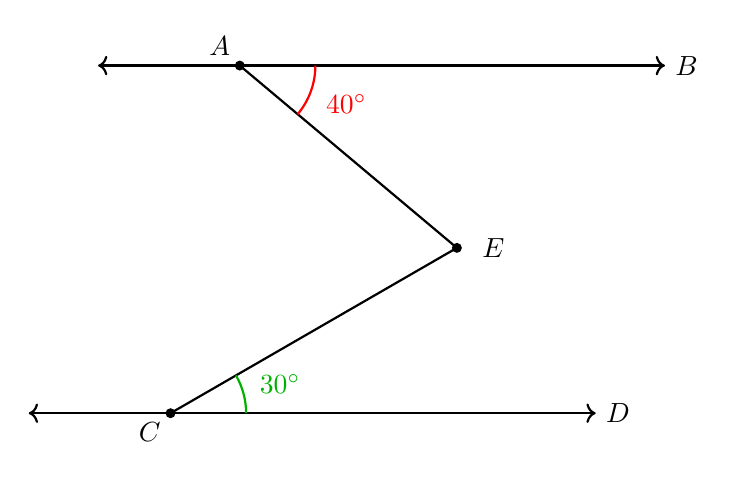
\begin{tikzpicture}[scale=1.2, font=\sffamily]

    % 1. Define the central bend point E
    \coordinate (E) at (4, 2);
    
    % 2. Define A and C based on the angles we want.
    % To make \angle BAE = 40^\circ with a horizontal line, A is placed 140^\circ from E.
    % To make \angle DCE = 30^\circ with a horizontal line, C is placed 210^\circ from E.
    \coordinate (A) at ($(E) + (140:3)$);
    \coordinate (C) at ($(E) + (210:3.5)$);
    
    % 3. Draw the top and bottom parallel lines passing through A and C
    \draw[thick, <->] ($(A) - (1.5,0)$) -- ($(A) + (4.5,0)$) node[right] {$B$};
    \draw[thick, <->] ($(C) - (1.5,0)$) -- ($(C) + (4.5,0)$) node[right] {$D$};
    
    % 4. Draw the auxiliary line through E
    %\draw[thick, blue, <->] ($(E) - (3,0)$) node[left] {$X$} -- ($(E) + (3,0)$) node[right] {$Y$};
    
    % 5. Draw the zig-zag transversal line
    \draw[thick] (A) -- (E) -- (C);
    
    % 6. Plot the points and label them
    \fill (A) circle (1.5pt) node[above left] {$A$};
    \fill (C) circle (1.5pt) node[below left] {$C$};
    \fill (E) circle (1.5pt) node[right, xshift=2mm] {$E$};
    
    % 7. Draw the given angles (40 and 30 degrees)
    % Angle BAE
    \draw[red, thick] (A) ++(0:0.8) arc (0:-40:0.8);
    \node[red] at ($(A) + (-20:1.2)$) {$40^\circ$};
    
    % Angle DCE
    \draw[green!70!black, thick] (C) ++(0:0.8) arc (0:30:0.8);
    \node[green!70!black] at ($(C) + (15:1.2)$) {$30^\circ$};
    
    % 8. Draw the alternate interior angles created by the auxiliary line
    % Angle 1 (Top part of AEC)
    %\draw[red, thick] (E) ++(180:0.6) arc (180:140:0.6);
    %\node[red] at ($(E) + (160:0.9)$) {$\angle 1$};
    
    % Angle 2 (Bottom part of AEC)
    %\draw[green!70!black, thick] (E) ++(180:0.6) arc (180:210:0.6);
    %\node[green!70!black] at ($(E) + (195:0.9)$) {$\angle 2$};

\end{tikzpicture}
    \end{center}
To compute this, we might consider drawing a line through $E$ which is parallel
to both $\overline{AB}$ and $\overline{CD}$, and call this point $X$.
\begin{center}
    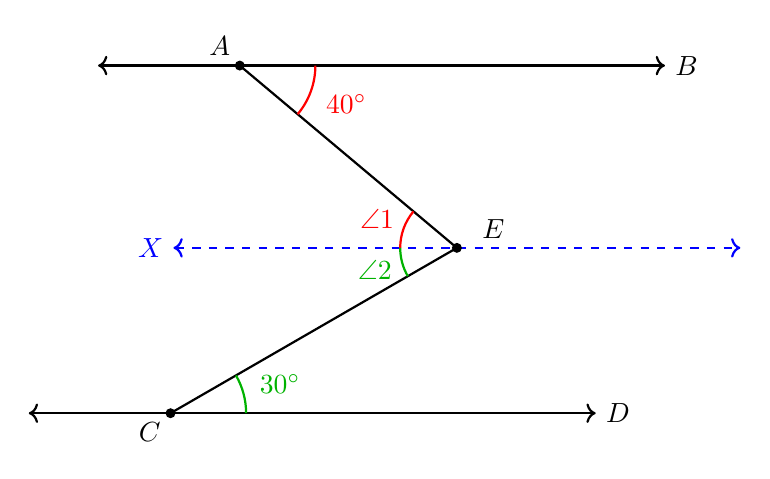
\begin{tikzpicture}[scale=1.2, font=\sffamily]

    % 1. Define the central bend point E
    \coordinate (E) at (4, 2);
    
    % 2. Define A and C based on the angles we want.
    % To make \angle BAE = 40^\circ with a horizontal line, A is placed 140^\circ from E.
    % To make \angle DCE = 30^\circ with a horizontal line, C is placed 210^\circ from E.
    \coordinate (A) at ($(E) + (140:3)$);
    \coordinate (C) at ($(E) + (210:3.5)$);
    
    % 3. Draw the top and bottom parallel lines passing through A and C
    \draw[thick, <->] ($(A) - (1.5,0)$) -- ($(A) + (4.5,0)$) node[right] {$B$};
    \draw[thick, <->] ($(C) - (1.5,0)$) -- ($(C) + (4.5,0)$) node[right] {$D$};
    
    % 4. Draw the auxiliary line through E
    \draw[thick, dashed, blue, <->] ($(E) - (3,0)$) node[left] {$X$} -- ($(E) + (3,0)$);
    
    % 5. Draw the zig-zag transversal line
    \draw[thick] (A) -- (E) -- (C);
    
    % 6. Plot the points and label them
    \fill (A) circle (1.5pt) node[above left] {$A$};
    \fill (C) circle (1.5pt) node[below left] {$C$};
    \fill (E) circle (1.5pt) node[above right, xshift=2mm] {$E$};
    
    % 7. Draw the given angles (40 and 30 degrees)
    % Angle BAE
    \draw[red, thick] (A) ++(0:0.8) arc (0:-40:0.8);
    \node[red] at ($(A) + (-20:1.2)$) {$40^\circ$};
    
    % Angle DCE
    \draw[green!70!black, thick] (C) ++(0:0.8) arc (0:30:0.8);
    \node[green!70!black] at ($(C) + (15:1.2)$) {$30^\circ$};
    
    % 8. Draw the alternate interior angles created by the auxiliary line
    % Angle 1 (Top part of AEC)
    \draw[red, thick] (E) ++(180:0.6) arc (180:140:0.6);
    \node[red] at ($(E) + (160:0.9)$) {$\angle 1$};
    
    % Angle 2 (Bottom part of AEC)
    \draw[green!70!black, thick] (E) ++(180:0.6) arc (180:210:0.6);
    \node[green!70!black] at ($(E) + (195:0.9)$) {$\angle 2$};
\end{tikzpicture}
\end{center}
Now using alternate interior angles we will have that $\angle1 = \angle  XEA =
40\degree$ and $\angle2 = \angle CEX = 30\degree$. Thus, we see that $\angle CEA
= \angle C E X  + \angle X E A = 30\degree+40\degree = 70\degree$. We would need
rules that would have to formalize how we are combining angles, but in practice
we will not need this rabbit as we will use linear algebra and AlphaGeometries
AR system will be able to do this computation without the need of the rabbit of
drawing the line through $X$.
\end{example}


\begin{remark}
    Again, this example shows another subtlety. Namely, the way in which we draw
    the diagram matters. We have drawn the diagram so that $AB$ and $CD$ are
    read left to right in alphabetical order. However, let us consider the same
    problem, but let us draw the diagram in a way in which the labels of $C$ and
    $D$ are in the opposite order.

    \begin{center}
        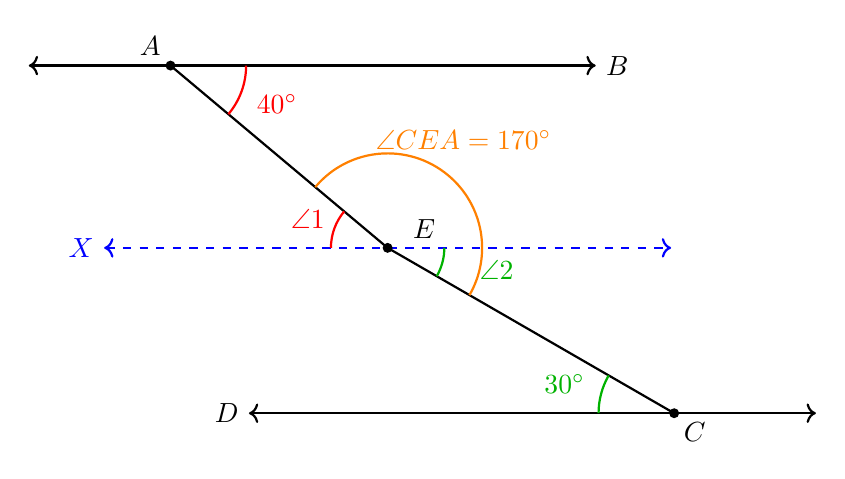
\begin{tikzpicture}[scale=1.2, font=\sffamily]

    % 1. Define the central bend point E
    \coordinate (E) at (4, 2);
    
    % 2. Define A and C based on the NEW angles.
    % To keep \angle BAE = 40^\circ (with B to the right), A is at 140^\circ from E.
    % To make \angle DCE = 30^\circ with D to the LEFT, C must be placed such that 
    % the ray CE is 30^\circ away from the left-pointing ray CD. 
    % We place C at -30^\circ (or 330^\circ) from E.
    \coordinate (A) at ($(E) + (140:3)$);
    \coordinate (C) at ($(E) + (-30:3.5)$);
    
    % 3. Draw the top parallel line (B is to the right of A)
    \draw[thick, <->] ($(A) - (1.5,0)$) -- ($(A) + (4.5,0)$) node[right] {$B$};
    
    % 4. Draw the bottom parallel line (D is now to the LEFT of C)
    \draw[thick, <->] ($(C) - (4.5,0)$) node[left] {$D$} -- ($(C) + (1.5,0)$);
    
    % 5. Draw the auxiliary line through E (X is left, Y is right)
    \draw[thick, dashed, blue, <->] ($(E) - (3,0)$) node[left] {$X$} -- ($(E) + (3,0)$);
    
    % 6. Draw the new transversal line
    \draw[thick] (A) -- (E) -- (C);
    
    % 7. Plot the points and label them
    \fill (A) circle (1.5pt) node[above left] {$A$};
    \fill (C) circle (1.5pt) node[below right] {$C$};
    \fill (E) circle (1.5pt) node[above right, xshift=2mm] {$E$};
    
    % 8. Draw the given angles (40 and 30 degrees)
    % Angle BAE (Remains the same)
    \draw[red, thick] (A) ++(0:0.8) arc (0:-40:0.8);
    \node[red] at ($(A) + (-20:1.2)$) {$40^\circ$};
    
    % NEW Angle DCE (Anchored to the left-pointing ray CD)
    \draw[green!70!black, thick] (C) ++(180:0.8) arc (180:150:0.8);
    \node[green!70!black] at ($(C) + (165:1.2)$) {$30^\circ$};
    
    % 9. Draw the NEW alternate interior angles
    % Angle 1 (Remains between EA and EX)
    \draw[red, thick] (E) ++(180:0.6) arc (180:140:0.6);
    \node[red] at ($(E) + (160:0.9)$) {$\angle 1$};
    
    % Angle 2 (Now alternate interior to the LEFT-facing angle, so it sits on the RIGHT)
    \draw[green!70!black, thick] (E) ++(0:0.6) arc (0:-30:0.6);
    \node[green!70!black] at ($(E) + (-15:0.9)$) [right]{$\angle 2$};

    % 10. Mark the actual target angle AEC to show it is no longer just 1+2
    \draw[thick, orange] (E) ++(140:1) arc (140:-30:1);
    \node[orange] at ($(E) + (55:1.4)$) {$\angle CEA = 170^\circ$};

\end{tikzpicture}
    \end{center}
We now see that the proof in which we gave is not true for the diagram above.
This shows the subtlety which must be taken into account when dealing with
angles. In particular, we will discuss different angle conventions which we
denote $\angle_0$ and $\angle_1$. We will discuss how $\angle_1$ which is the
angle between two lines modulo $\pi$ (or $180\degree)$ will be the one in which
AlphaGeometry and our systems use.
\end{remark}

\begin{example}
    Now let us consider the following example, consider a circle with center $O$
    and $ABC$ lying on the circle. We wish to show that $\angle BOC=2\angle
    BAC$.

    \begin{center}
        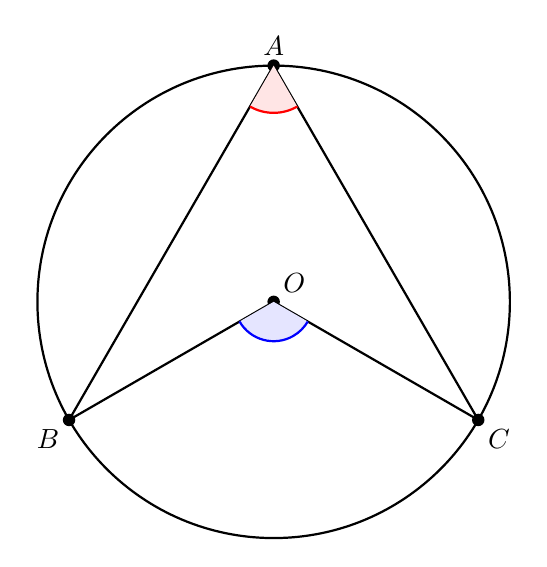
\begin{tikzpicture}[scale=1.5, font=\sffamily]
    
    % 1. Define the coordinates
    % We place A at the top, and B/C at the bottom to form the arrowhead
    \coordinate (O) at (0,0);
    \coordinate (A) at (90:2);
    \coordinate (B) at (210:2);
    \coordinate (C) at (330:2);

    % 2. Draw the main circle
    \draw[thick] (O) circle (2);

    % 3. Draw the inscribed angle (BAC) and the central angle (BOC)
    \draw[thick] (B) -- (A) -- (C);
    \draw[thick] (B) -- (O) -- (C);

    % 4. Plot the points and label them
    \fill (O) circle (1.5pt) node[above right] {$O$};
    \fill (A) circle (1.5pt) node[above] {$A$};
    \fill (B) circle (1.5pt) node[below left] {$B$};
    \fill (C) circle (1.5pt) node[below right] {$C$};

    % 5. Highlight the two target angles to show the goal
    \pic [draw, thick, red, angle radius=0.6cm, fill=red!10] {angle = B--A--C};
    \pic [draw, thick, blue, angle radius=0.5cm, fill=blue!10] {angle = B--O--C};

\end{tikzpicture}
    \end{center}

    We formalize this problem as follows:
    \begin{itemize}
        \item \verb|[1] circle O A B C| (this says that $O$ is the circumcenter of triangle $ABC$)
        \item \lstinline|[?] angeq C A A B C O O B 2 -2 -1 1 0| (this is asking if $2d(CA)-2d(AB)-d(CO)+d(OB)=0$ we will define the function $d$ later when we talk about our angle conventions. In particular, we will have that $d(CA)-d(AB)=\angle CAB$ Thus, this is asking if $\angle BOC = 2\angle BAC$)
    \end{itemize}

    Now to solve this problem, we can consider the rabbit of drawing the line
    from $A$ to $O$ intersecting the circle at a new point $D$.

    \begin{center}
        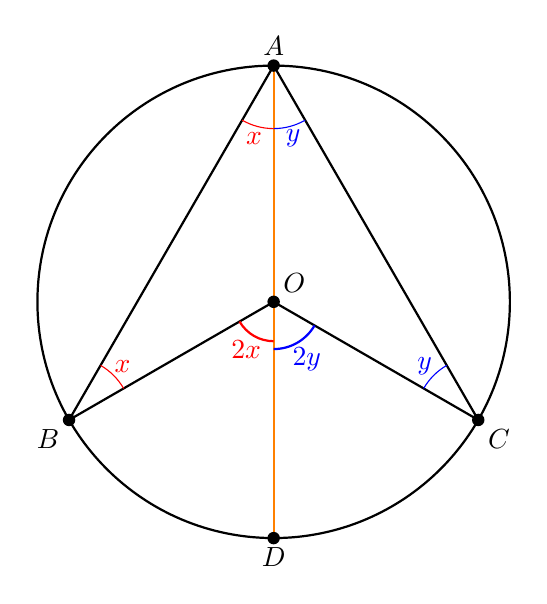
\begin{tikzpicture}[scale=1.5, font=\sffamily]
    
    % 1. Define the coordinates
    \coordinate (O) at (0,0);
    \coordinate (A) at (90:2);
    \coordinate (B) at (210:2);
    \coordinate (C) at (330:2);
    
    % Define point D dynamically as the exact opposite of A through O
    \coordinate (D) at ($(O)!-1!(A)$);

    % 2. Draw the main circle
    \draw[thick] (O) circle (2);

    % 3. Draw the original Star Trek lines
    \draw[thick] (B) -- (A) -- (C);
    \draw[thick] (B) -- (O) -- (C);

    % 4. Draw the MAGIC AUXILIARY LINE
    % Drawn dashed to show it's a construction
    \draw[thick, orange] (A) -- (D);

    % 5. Plot the points and label them
    \fill (O) circle (1.5pt) node[above right] {$O$};
    \fill (A) circle (1.5pt) node[above] {$A$};
    \fill (B) circle (1.5pt) node[below left] {$B$};
    \fill (C) circle (1.5pt) node[below right] {$C$};
    \fill (D) circle (1.5pt) node[below] {$D$};

    % 6. Mark the equal angles in the LEFT isosceles triangle (AOB)
    \pic [draw, red, "$x$", angle radius=0.8cm, angle eccentricity=1.2] {angle = B--A--O};
    \pic [draw, red, "$x$", angle radius=0.8cm, angle eccentricity=1.2] {angle = O--B--A};
    
    % Mark the exterior angle for the left triangle
    \pic [draw, red, thick, "$2x$", angle radius=0.5cm, angle eccentricity=1.4] {angle = B--O--D};

    % 7. Mark the equal angles in the RIGHT isosceles triangle (AOC)
    \pic [draw, blue, "$y$", angle radius=0.8cm, angle eccentricity=1.2] {angle = O--A--C};
    \pic [draw, blue, "$y$", angle radius=0.8cm, angle eccentricity=1.2] {angle = A--C--O};
    
    % Mark the exterior angle for the right triangle
    \pic [draw, blue, thick, "$2y$", angle radius=0.6cm, angle eccentricity=1.4] {angle = D--O--C};

\end{tikzpicture}
    \end{center}

    Now once we draw this line, we observe that we will have isoceles triangles
    $ABO$ and $ACO$ with angles $x$ and $y$ respectively. We then have $\angle
    BOA = 180\degree - 2x$, so $\angle BOD = 2x$. Similarly, $\angle COA =
    180\degree - 2y$, so $\angle COD = 2y$. Hence, $\angle BOC = 2x+2y$.
    Similarly, we see that $\angle BAO = x$, $\angle CAO = y$, so $\angle BAC =
    \angle BAO + \angle CAO = x+y$. Thus, we have solved the problem.

\end{example}

\section{Architecture of Our System}
In this section, we will give a giant overview of all the files which we shall
be creating through the course of the semester, and their purpose.

\textcolor{red}{WRITE THIS ONCE TO BLUEPRINT EVERYTHING}

\section{Angle Conventions}

We begin by talking about the different angle conventions that one may take, and
what we truly mean by an angle in terms of our system. In practice, we will
consider the angle measured between two lines counter-clockwise modulo $\pi$.

\subsection{Angle 0}

\begin{defn}
    We define $\angle_0 ABC$ to be the traditional angle measured between the
    segment $AB$ and the segment $BC$.
    \begin{center}
    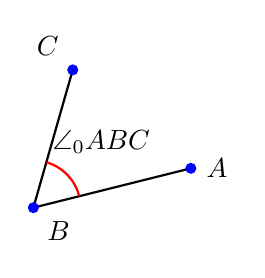
\begin{tikzpicture}[scale=.5,
        % Define a style for the points
        point/.style={fill=blue, circle, minimum size=4pt, inner sep=0pt}]

        % 1. Define the coordinates for the points
        \coordinate (A) at (4, 1);
        \coordinate (B) at (0, 0); % The vertex of the angle
        \coordinate (C) at (1, 3.5);

        % 2. Draw the segments (lines) forming the angle
        \draw[thick] (A) -- (B) -- (C);

        % 3. Mark the points and label them
        \node[point, label={below right:$B$}] at (B) {};
        \node[point, label={right:$A$}] at (A) {};
        \node[point, label={above left:$C$}] at (C) {};

        % 4. Mark the angle ABC
        
        % The 'angle' style requires the 'quotes' and 'angles' libraries.
        % The format is: \draw (Point A) -- (Vertex B) -- (Point C);
        \pic["$\angle_0ABC$", draw=red, thick, angle eccentricity=2, angle radius=0.6cm] {angle = A--B--C};
    \end{tikzpicture}
    \end{center}
    One limitation of this definition is that when we want to calculate the
    angle between two lines, it the measurement of the angle depends upon which
    side of the line the point lies on. In particular, we see that if $A$ and
    $A'$ lie on opposite sides of the line, then $\angle_0ABC\neq\angle_0A'BC$
    (although, we will have that $\angle_0ABC + \angle_0A'BC=\pi$, see the
    figure below). Thus, if we wanted to use the convention of $\angle_0$, then
    for a given line, we would need to keep track of the order of the points
    appearing (this is possible, but more complicated to implement for the
    computer).

    \begin{center}
        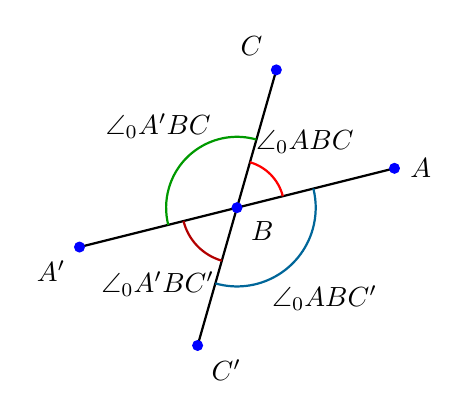
\begin{tikzpicture}[scale=.5,
        % Define a style for the points
        point/.style={fill=blue, circle, minimum size=4pt, inner sep=0pt}]

        % 1. Define the coordinates for the four outer points
        \coordinate (B) at (0, 0); % The central vertex
        
        % Line 1: A to A'
        \coordinate (A) at (4, 1);
        \coordinate (Aprime) at (-4, -1); % A' is reflection of A through B
        
        % Line 2: C to C'
        \coordinate (C) at (1, 3.5);
        \coordinate (Cprime) at (-1, -3.5); % C' is reflection of C through B

        % 2. Draw the two intersecting lines
        \draw[thick] (Aprime) -- (A); % Line A'A (lighter)
        \draw[thick] (Cprime) -- (C); % Line C'C (slightly colored)

        % 3. Mark the points and label them
        \node[point, label={below right:$B$}] at (B) {};
        \node[point, label={right:$A$}] at (A) {};
        \node[point, label={above left:$C$}] at (C) {};
        \node[point, label={below left:$A'$}] at (Aprime) {};
        \node[point, label={below right:$C'$}] at (Cprime) {};


        % 4. Mark Angle 1: alpha (Vertically opposite to gamma)
        % Angle: A -- B -- C
        \pic ["$\angle_0 A BC$", draw=red, thick, angle eccentricity=2, angle radius=0.6cm] {angle = A--B--C};

        % 5. Mark Angle 2: beta (Adjacent to alpha)
        % Angle: C -- B -- A'
        \pic ["$\angle_0A'BC$", draw=green!60!black, thick, angle eccentricity=1.6, angle radius=0.9cm] {angle = C--B--Aprime};
        
        % 6. Mark Angle 3: gamma (Vertically opposite to alpha, should be equal)
        % Angle: A' -- B -- C'
        \pic ["$\angle_0A'BC'$", draw=red!70!black, thick, angle eccentricity=2, angle radius=0.7cm] {angle = Aprime--B--Cprime};
        
        % 7. Mark Angle 4: delta (Vertically opposite to beta, should be equal)
        % Angle: C' -- B -- A
        \pic ["$\angle_0ABC'$", draw=green!40!blue, thick, angle eccentricity=1.6, angle radius=1.0cm] {angle = Cprime--B--A};

    \end{tikzpicture}
    \end{center}
\end{defn}
Now we see that the range of $\angle_0$ is $(0,\pi)$. We also have that
$\angle_0$ satisfies $\angle_0ABC = \angle_0CBA$. Now in terms of $\angle_0$,
the statement that the sum of the angles of a triangle add up to $\pi$ can be
interpreted as the following proposition.

\begin{prop}
    Given a triangle $ABC$, then $\angle_0ABC + \angle_0BCA + \angle_0CAB =
    \pi$.
\end{prop}
This is seen by drawing the picture of the triangle, and just labeling the
angles. Furthermore, we remark that this statement is independent of the
orientation of the points $ABC$ as $\angle_0ABC = \angle_0CBA$. In the below,
the blue triangle on the left shows this in the case where the ordered points
$ABC$ are positively oriented, and the red triangle on the right shows this in
the case where the ordered points $ABC$ are negatively oriented.
\begin{center}
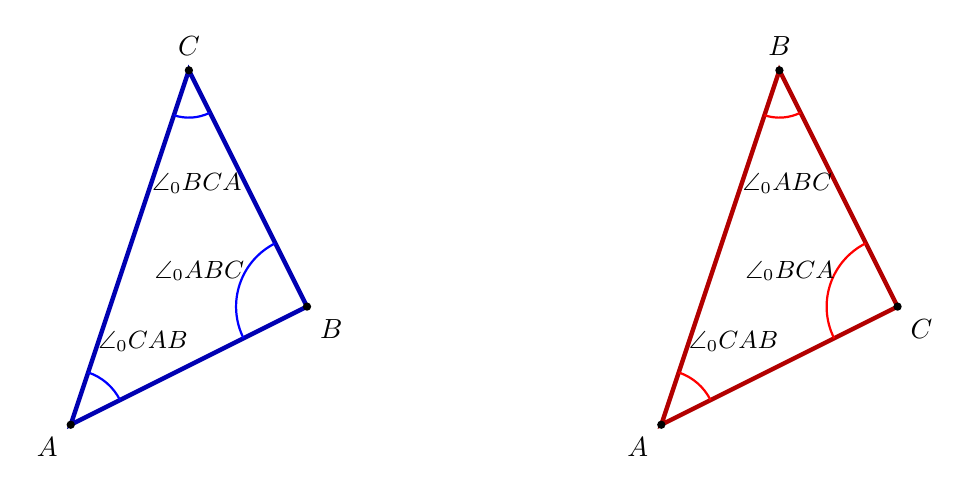
\begin{tikzpicture}[scale=1.5]

        % Style for vertices
        \tikzset{vertex/.style={fill=black, circle, minimum size=3pt, inner sep=0pt}}

        % =================================================================
        % 1. POSITIVE ORIENTATION (Counter-Clockwise) - Left Triangle
        % =================================================================
        
        \begin{scope}[shift={(0,0)}]

            % Define Coordinates
            \coordinate (A) at (1, 1);
            \coordinate (B) at (3, 2);
            \coordinate (C) at (2, 4);

            % Draw the triangle (no shading requested)
            % Drawing the path CCW (A -> B -> C -> A)
            \draw[blue!70!black, ultra thick] (A) -- (B) -- (C) -- cycle;
            
            % Label the vertices
            \node[vertex, label={below left:$A$}] at (A) {};
            \node[vertex, label={below right:$B$}] at (B) {};
            \node[vertex, label={above:$C$}] at (C) {};
            
            % Mark the Angles
            % Angle alpha at A (B--A--C)
            \pic ["{\small $\angle_0CAB$}", draw=blue,thick, angle eccentricity=2, angle radius=0.7cm] {angle = B--A--C};
            % Angle beta at B (C--B--A)
            \pic ["{\small $\angle_0ABC$}", draw=blue, thick, angle eccentricity=1.6, angle radius=0.9cm] {angle = C--B--A};
            % Angle gamma at C (A--C--B)
            \pic ["{\small $\angle_0BCA$}", draw=blue, thick, angle eccentricity=2.4, angle radius=0.6cm] {angle = A--C--B};
            
        \end{scope}


        % =================================================================
        % 2. NEGATIVE ORIENTATION (Clockwise) - Right Triangle
        % =================================================================

        \begin{scope}[shift={(5,0)}] % Shift 7 units to the right
    % Define Coordinates
            \coordinate (A) at (1, 1);
            \coordinate (B) at (2, 4);
            \coordinate (C) at (3, 2);

            % Draw the triangle (no shading requested)
            % Drawing the path CCW (A -> B -> C -> A)
            \draw[red!70!black, ultra thick] (A) -- (B) -- (C) -- cycle;
            
            % Label the vertices
            \node[vertex, label={below left:$A$}] at (A) {};
            \node[vertex, label={above:$B$}] at (B) {};
            \node[vertex, label={below right:$C$}] at (C) {};
            
            % Mark the Angles
            % Angle alpha at A (B--A--C)
            \pic ["{\small $\angle_0CAB$}", draw=red,thick, angle eccentricity=2, angle radius=0.7cm] {angle = C--A--B};
            % Angle beta at B (C--B--A)
            \pic ["{\small $\angle_0BCA$}", draw=red, thick, angle eccentricity=1.6, angle radius=0.9cm] {angle = B--C--A};
            % Angle gamma at C (A--C--B)
            \pic ["{\small $\angle_0ABC$}", draw=red, thick, angle eccentricity=2.4, angle radius=0.6cm] {angle = A--B--C};
            
        \end{scope}
    \end{tikzpicture}
\end{center}

Now we remark that given parallel lines, if a third line passes through the two,
then there are some statements on how some angles will be the equal. We state
these rules below in terms of $\angle_0$. It is worth noting that these
statements can get quite complicated where we must describe the relationship of
different points to one another. This is one down side of the $\angle_0$ in that
for a human it can be clear when two angles are equal, but for a computer there
would be a lot of things to check to apply these angle congruences.

\begin{prop}[Corresponding Angles]\label{prop: Corresonding Angles for Angle 0}
    Say that the lines $AB$ and $A'B'$ are parallel and say that $BB'C$ are
    collinear such that $A$ and $A'$ lie on the same side of the plane with
    respect to the line $BB'C$, and $C$ does not lie between $B$ and $B'$, then
    $\angle_0ABC = \angle_0A'B'C$.

    \noindent (Note: the picture below is the case where $B$ lies between $B'$
    and $C$, but you may convince yourself that the statement is still true if
    instead $B'$ is between $B$ and $C$ (that is if $C$ is on the other end of
    the line)
\end{prop}

\begin{center}
    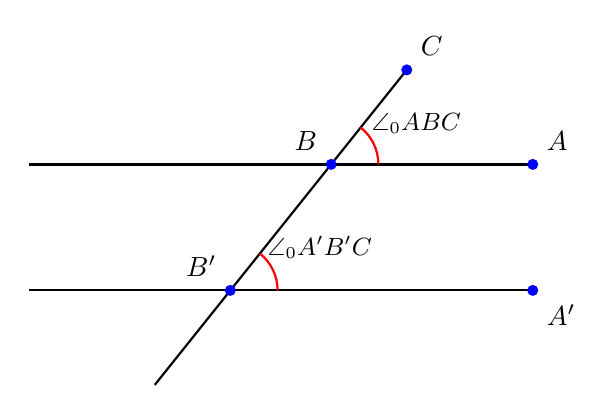
\begin{tikzpicture}[scale=.8]

        % 1. Define the coordinates and drawing limits
        \pgfmathsetmacro{\xshift}{4} % Horizontal span for the lines
        \pgfmathsetmacro{\yshift}{2}  % Vertical distance between parallel lines
        
        \coordinate (TL) at (-\xshift, \yshift); % Top Left
        \coordinate (TR) at (\xshift, \yshift);  % Top Right (Used as A coordinate)
        \coordinate (BL) at (-\xshift, 0);       % Bottom Left
        \coordinate (BR) at (\xshift, 0);        % Bottom Right (Used as A' coordinate)

        % Transversal line coordinates
        \coordinate (TransA) at (0.5*\xshift, \yshift + 1.5);
        \coordinate (TransB) at (-0.5*\xshift, -1.5);

        % Calculate intersection points (B and B')
        \coordinate (B) at (intersection of TL--TR and TransA--TransB);
        \coordinate (Bprime) at (intersection of BL--BR and TransA--TransB);
        
        % Define point C on the transversal (using the coordinate provided in your code)
        \coordinate (C_coord) at ($(B)!0.3!(TransA)$); % Renamed to avoid clash with angle C in general geometry

        % 2. Draw the Parallel Lines (A and A') - ALL BLACK
        % Line A
        \draw[thick, black] (TL) -- (TR);
        % Line A'
        \draw[thick, black] (BL) -- (BR);

        % 3. Draw the Transversal Line (T) - ALL BLACK
        \draw[thick, black] (TransA) -- (TransB);
        
        % 4. Mark Intersections (B and B') and Points A, A', and C
        \tikzset{vertex/.style={fill=blue, circle, minimum size=4pt, inner sep=0pt}} % Set vertex style to blue circle

        % Mark A and A' (now explicitly defined nodes at the right end)
        \node[vertex, label={above right:$A$}] at (TR) {}; 
        \node[vertex, label={below right:$A'$}] at (BR) {};
        
        % Mark B and B' (Intersections)
        \node[vertex, label={above left:$B$}] at (B) {};
        \node[vertex, label={above left:$B'$}] at (Bprime) {};
        
        % Mark C (on Transversal)
        \node[vertex, label={above right:$C$}] at (TransA) {};


        % 5. Mark Corresponding Angles (alpha = alpha)
        \def\angleRadius{0.6cm}
        
        % Angle Alpha 1 (Top-Left position at intersection B)
        % Defined by the top parallel line and the transversal (TR--B--TransA)
        \pic ["{\small $\angle_0 A B C$}", draw=red, thick, angle eccentricity=2, angle radius=\angleRadius] {angle = TR--B--TransA};

        % Angle Alpha 2 (Top-Left position at intersection B')
        % Defined by the bottom parallel line and the transversal (BR--B'--TransB)
        \pic ["{\small $\angle_0 A' B' C$}", draw=red, thick, angle eccentricity=2.1, angle radius=\angleRadius] {angle = BR--Bprime--TransA};

    \end{tikzpicture}
\end{center}

\begin{prop}[Alternate Interior Angles]
    Say that the line $AB$ and $A'B'$ are parallel and say that $BCB'$ are
    collinear such that $A$ and $A'$ lie on the opposite sides of the plane with
    respect to the line $BCB'$, and if $C$ lies between $B$ and $B'$, then
    $\angle_0ABC = \angle_0A'B'C$.
\end{prop}

\begin{center}
    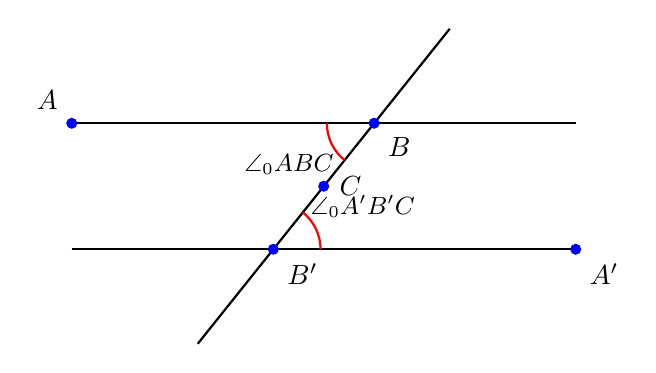
\begin{tikzpicture}[scale=.8]

        % 1. Define the coordinates and drawing limits
        \pgfmathsetmacro{\xshift}{4} % Horizontal span for the lines
        \pgfmathsetmacro{\yshift}{2}  % Vertical distance between parallel lines
        
        \coordinate (TL) at (-\xshift, \yshift); % Top Left (for Node A)
        \coordinate (TR) at (\xshift, \yshift);  % Top Right
        \coordinate (BL) at (-\xshift, 0);       % Bottom Left
        \coordinate (BR) at (\xshift, 0);        % Bottom Right (for Node A')

        % Transversal line coordinates
        \coordinate (TransA) at (0.5*\xshift, \yshift + 1.5);
        \coordinate (TransB) at (-0.5*\xshift, -1.5);

        % Calculate intersection points (B and B')
        \coordinate (B) at (intersection of TL--TR and TransA--TransB);
        \coordinate (Bprime) at (intersection of BL--BR and TransA--TransB);
        
        % Define point C as the midpoint between B and B'
        \coordinate (C) at ($(B)!0.5!(Bprime)$);

        % 2. Draw the Parallel Lines (A and A') - ALL BLACK
        % Line A
        \draw[thick, black] (TL) -- (TR);
        % Line A'
        \draw[thick, black] (BL) -- (BR);

        % 3. Draw the Transversal Line (T) - ALL BLACK
        \draw[thick, black] (TransA) -- (TransB);
        
        % 4. Mark Intersections (B and B') and Points A, A', and C
        \tikzset{vertex/.style={fill=blue, circle, minimum size=4pt, inner sep=0pt}} % Set vertex style to blue circle

        % Mark A (at the LEFT end)
        \node[vertex, label={above left:$A$}] at (TL) {}; 
        % Mark A' (at the RIGHT end)
        \node[vertex, label={below right:$A'$}] at (BR) {};
        
        % Mark B and B' (Intersections)
        \node[vertex, label={below right:$B$}] at (B) {};
        \node[vertex, label={below right:$B'$}] at (Bprime) {};
        
        % Mark C (Midpoint between B and B')
        \node[vertex, label={right:$C$}] at (C) {};


        % 5. Mark Alternate Interior Angles (gamma = gamma')
        \def\angleRadius{0.6cm}
        
        % Angle Gamma 1 (Upper Interior, Right side of Transversal at B)
        % Defined by the top parallel line and the transversal (TransA--B--TL)
        \pic ["{\small $\angle_0 ABC$}", draw=red, thick, angle eccentricity=2, angle radius=\angleRadius] {angle = TL--B--C};

        % Angle Gamma 2 (Lower Interior, Left side of Transversal at B')
        % Defined by the bottom parallel line and the transversal (BL--B'--TransB)
        \pic ["{\small $\angle_0A'B'C$}", draw=red, thick, angle eccentricity=2.1, angle radius=\angleRadius] {angle = BR--Bprime--C};

    \end{tikzpicture}
\end{center}

\begin{prop}[Alternate Exterior Angles]
    Say that the lines $AB$ and $A'B'$ are parallel and say that $C'B'BC$ are
    collinear such that $A$ and $A'$ lie on opposite sides of plane with respect
    to the line $C'B'BC$. Furthermore, suppose that $B'$ is between $C'$ and
    $B$, and that $B$ is between $C$ and $B'$, then $\angle_0ABC =
    \angle_0A'B'C'$.
\end{prop}

\begin{center}
    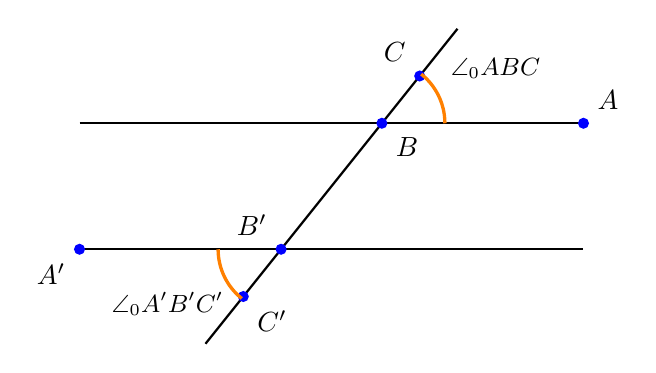
\begin{tikzpicture}[scale=.8]

        % 1. Define the coordinates and drawing limits
        \pgfmathsetmacro{\xshift}{4} % Horizontal span for the lines
        \pgfmathsetmacro{\yshift}{2}  % Vertical distance between parallel lines
        
        \coordinate (TL) at (-\xshift, \yshift); % Top Left
        \coordinate (TR) at (\xshift, \yshift);  % Top Right (for Node A)
        \coordinate (BL) at (-\xshift, 0);       % Bottom Left (for Node A')
        \coordinate (BR) at (\xshift, 0);        % Bottom Right

        % Transversal line coordinates
        \coordinate (TransA) at (0.5*\xshift, \yshift + 1.5); % Top end of transversal
        \coordinate (TransB) at (-0.5*\xshift, -1.5); % Bottom end of transversal

        % Calculate intersection points (B and B')
        \coordinate (B) at (intersection of TL--TR and TransA--TransB);
        \coordinate (Bprime) at (intersection of BL--BR and TransA--TransB);
        
        % Define C (on transversal, top exterior region)
        \coordinate (C) at ($(B)!0.5!(TransA)$);
        % Define C' (on transversal, bottom exterior region)
        \coordinate (Cprime) at ($(Bprime)!0.5!(TransB)$);

        % 2. Draw the Parallel Lines - ALL BLACK
        \draw[thick, black] (TL) -- (TR);
        \draw[thick, black] (BL) -- (BR);

        % 3. Draw the Transversal Line - ALL BLACK
        \draw[thick, black] (TransA) -- (TransB);
        
        % 4. Mark Intersections (B and B') and Points A, A', C, C'
        \tikzset{vertex/.style={fill=blue, circle, minimum size=4pt, inner sep=0pt}} % Set vertex style to blue circle

        % Mark A (Top Right)
        \node[vertex, label={above right:$A$}] at (TR) {}; 
        % Mark A' (Bottom Left)
        \node[vertex, label={below left:$A'$}] at (BL) {};
        
        % Mark B and B' (Intersections)
        \node[vertex, label={below right:$B$}] at (B) {};
        \node[vertex, label={above left:$B'$}] at (Bprime) {};
        
        % Mark C (Top Exterior, on Transversal)
        \node[vertex, label={above left:$C$}] at (C) {};
        % Mark C' (Bottom Exterior, on Transversal)
        \node[vertex, label={below right:$C'$}] at (Cprime) {};


        % 5. Mark Alternate Exterior Angles (delta = delta')
        \def\angleRadius{0.8cm}
        
        % Angle Delta 1 (Top Exterior, Left side of Transversal at B)
        % Defined by the top parallel line and the transversal (TL--B--TransB)
        \pic ["{\small $\angle_0ABC$}", draw=orange, very thick, angle eccentricity=2, angle radius=\angleRadius] {angle = TR--B--TransA};

        % Angle Delta 2 (Bottom Exterior, Right side of Transversal at B')
        % Defined by the bottom parallel line and the transversal (TransA--Bprime--BR)
        \pic ["{\small $\angle_0A'B'C'$}", draw=orange, very thick, angle eccentricity=2, angle radius=\angleRadius] {angle = BL--Bprime--TransB};

    \end{tikzpicture}
\end{center}


\begin{prop}[Vertical Angles]
    Given lines $A'BA$ and $C'BC$ such that $B$ lies between $A$ and $A'$ on the
    line $ABA'$ and $B$ lies between $C$ and $C'$ on the line $CBC'$
    (equivalently if $A$ and $A'$ are on opposite sides of the plane with
    respect to the line $CBC'$ and similar with $C$ and $C'$ with the line
    $ABA'$), then $\angle_0ABC=\angle_0A'BC'$.
\end{prop}

\begin{center}
    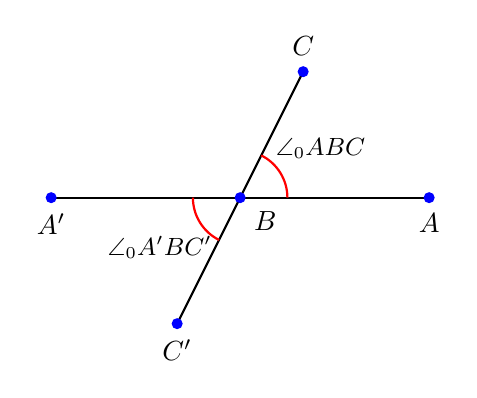
\begin{tikzpicture}[scale=.8]

        % Define the vertex (B)
        \coordinate (B) at (0, 0);

        % 1. Define Line 1 (A' B A, left to right) - Horizontal
        \coordinate (Aprime) at (-3, 0); % A' (Left)
        \coordinate (A) at (3, 0);       % A (Right)
        
        % 2. Define Line 2 (C B C', top to bottom) - SLANTED (Non-Perpendicular)
        % Coordinates adjusted to create an acute/obtuse intersection
        \coordinate (C) at (1, 2);       % C (Top-Right slant)
        \coordinate (Cprime) at (-1, -2); % C' (Bottom-Left slant)

        % 3. Draw the two intersecting lines - ALL BLACK
        % Line A'A
        \draw[ thick, black] (Aprime) -- (A);
        % Line C C'
        \draw[ thick, black] (C) -- (Cprime);
        
        % 4. Mark all points (A, A', C, C', B)
        \tikzset{vertex/.style={fill=blue, circle, minimum size=4pt, inner sep=0pt}}

        \node[vertex, label={below:$A$}] at (A) {};
        \node[vertex, label={below:$A'$}] at (Aprime) {};
        
        \node[vertex, label={above:$C$}] at (C) {};
        \node[vertex, label={below:$C'$}] at (Cprime) {};
        
        \node[vertex, label={below right:$B$}] at (B) {}; % Vertex B

        % 5. Mark the two pairs of vertical angles

        \def\radiusAlpha{0.8cm}
        \def\radiusBeta{0.6cm}
        
        % PAIR 1: Vertical Angles alpha (Acute angle)
        % Angle alpha (A--B--C) - Top Right (Acute)
        \pic ["{\small $\angle_0 ABC$}", draw=red, thick, angle eccentricity=2, angle radius=\radiusBeta] {angle = A--B--C};
        
        % Angle alpha' (C'--B--A') - Bottom Left (Acute, Vertically Opposite)
        %\pic ["{\small $\alpha$}", draw=red, thick, angle eccentricity=1.2, angle radius=\radiusAlpha] {angle = Cprime--B--Aprime};
        
        
        % PAIR 2: Vertical Angles beta (Obtuse angle)
        % Angle beta (C--B--A') - Top Left (Obtuse)
        % Using a smaller radius so it fits cleanly
        %\pic ["{\small $\beta$}", draw=orange, thick, angle eccentricity=1.3, angle radius=\radiusBeta] {angle = Cprime--B--Aprime};

        % Angle beta' (A--B--C') - Bottom Right (Obtuse, Vertically Opposite)
        \pic ["{\small $\angle_0 A'BC'$}", draw=red, thick, angle eccentricity=2, angle radius=\radiusBeta] {angle = Aprime--B--Cprime};

    \end{tikzpicture}
\end{center}

\begin{defn}\label{defn: congruent triangles}
    Two triangles $\triangle ABC$ and $\triangle DEF$ are congruent if $AB =
    DE$, $BC = EF$, $CA = FD$, $\angle_0ABC = \angle_0DEF$, $\angle_0BCA =
    \angle_0EFD$, and $\angle_0CAB = \angle_0FDE$.
\end{defn}
\noindent We have some classical results involving triangles. 
\begin{prop}[Euclid Book I Prop 4]\label{prop: Euclid Book 1 Prop 4 Angle 0} 
    If $AB = DE$, $BC = EF$, $\angle_0 ABC = \angle_0DEF$, then $\triangle ABC$
    and $\triangle DEF$ are congruent. This is the classical ``side-angle-side''
    triangle congruence rule.
\end{prop}

\begin{prop}[Euclid Book I Prop 5]\label{prop: Euclid Book 1 Prop 5 Angle 0}
    If $AB = AC$, then $\angle_0ABC = \angle_0ACB$. 
\end{prop}


\subsection{Angle 1}

Now we will describe a different way of measuring angles. This will be the
measurement that we will use when building our AI. In particular, it will be
important to see that there are differences in the statements of the
propositions between the different kinds of angle conventions.

\begin{defn}
    We define $\angle_1 ABC$ to be the angle measured between line $AB$ and line
    $BC$ where we measure the angle counter-clockwise from the line $AB$ to the
    line $BC$.
    \begin{center}
        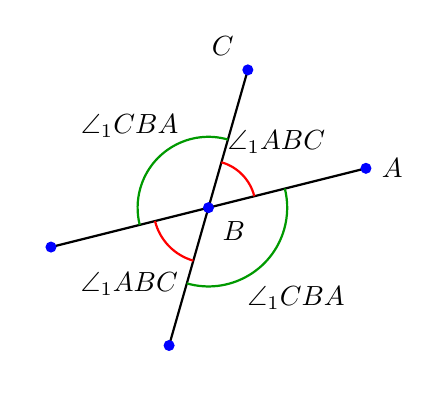
\begin{tikzpicture}[scale=.5,
        % Define a style for the points
        point/.style={fill=blue, circle, minimum size=4pt, inner sep=0pt}]

        % 1. Define the coordinates for the four outer points
        \coordinate (B) at (0, 0); % The central vertex
        
        % Line 1: A to A'
        \coordinate (A) at (4, 1);
        \coordinate (Aprime) at (-4, -1); % A' is reflection of A through B
        
        % Line 2: C to C'
        \coordinate (C) at (1, 3.5);
        \coordinate (Cprime) at (-1, -3.5); % C' is reflection of C through B

        % 2. Draw the two intersecting lines
        \draw[thick] (Aprime) -- (A); % Line A'A (lighter)
        \draw[thick] (Cprime) -- (C); % Line C'C (slightly colored)

        % 3. Mark the points and label them
        \node[point, label={below right:$B$}] at (B) {};
        \node[point, label={right:$A$}] at (A) {};
        \node[point, label={above left:$C$}] at (C) {};
        \node[point, label={below left:$ $}] at (Aprime) {};
        \node[point, label={below right:$ $}] at (Cprime) {};


        % 4. Mark Angle 1: alpha (Vertically opposite to gamma)
        % Angle: A -- B -- C
        \pic ["$\angle_1 A BC$", draw=red, thick, angle eccentricity=2, angle radius=0.6cm] {angle = A--B--C};

        % 5. Mark Angle 2: beta (Adjacent to alpha)
        % Angle: C -- B -- A'
        \pic ["$\angle_1CBA$", draw=green!60!black, thick, angle eccentricity=1.6, angle radius=0.9cm] {angle = C--B--Aprime};
        
        % 6. Mark Angle 3: gamma (Vertically opposite to alpha, should be equal)
        % Angle: A' -- B -- C'
        \pic ["$\angle_1ABC$", draw=red, thick, angle eccentricity=2, angle radius=0.7cm] {angle = Aprime--B--Cprime};
        
        % 7. Mark Angle 4: delta (Vertically opposite to beta, should be equal)
        % Angle: C' -- B -- A
        \pic ["$\angle_1CBA$", draw=green!60!black, thick, angle eccentricity=1.6, angle radius=1.0cm] {angle = Cprime--B--A};

    \end{tikzpicture}
    \end{center}
    We see that $\angle_1$ will take values of angles between $0$ and $\pi$ or
    $0$ and $180\degree$. We shall call this the unsigned angle modulo $\pi$ or
    the unsigned angle modulo $180\degree$.
\end{defn}

\begin{remark}
    We say it is modulo $\pi$ or $180\degree$ since after rotating the line, any
    additional rotation by any multiple of $\pi$ or $180\degree$ will be the
    same. Later on we will see that this modulo $\pi$ condition is needed when
    we have that $\angle_1 ABC = d(AB) -d(BC)$ which is only true if we consider
    things moduluo $\pi$.
\end{remark}

The big advantage of defining $\angle_1$ is that this definition of angle just
measures the angle between two lines. Now we see that in the definition of
$\angle_1$, it is independent of where the point is on the line. However, it
depends on the order of the lines. We see that $\angle_1ABC+\angle_1CBA = \pi$.
Thus, in general $\angle_1ABC \neq \angle_1 CBA$.

The first advantage that we see when looking at $\angle_1$ is that the statement
of the vertical angles is now clearly true as we are just measuring the angle
between two lines, we will have that the statement of vertical angles is just
$\angle_1ABC = \angle_1ABC$, so we do not need to include this proposition.

The next advantage of $\angle_1$, when we look at parallel lines then the
Corresponding Angles, Alternate Interior Angles, and Alternate Exterior Angles
propositions can be combined into a single statement.

\begin{prop}[Corresponding Angles, Alternate Interior Angles, and Alternate
Exterior Angles. ]
    Let lines $AB$ and $A'B'$ be parallel and let $BB'C$ be collinear (where the
    location of $C$ need not matter). Then $\angle_1ABC=\angle_1A'B'C$.
\end{prop}

\begin{center}
    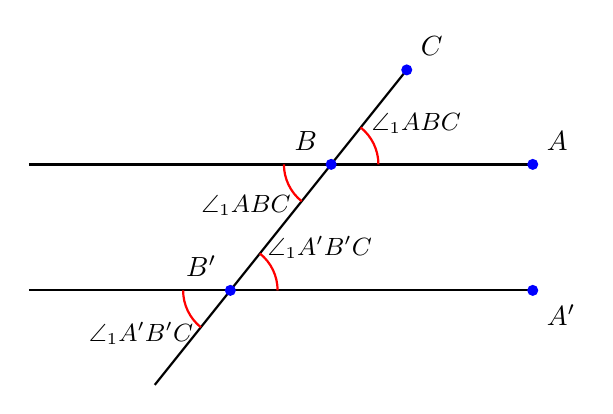
\begin{tikzpicture}[scale=.8]

        % 1. Define the coordinates and drawing limits
        \pgfmathsetmacro{\xshift}{4} % Horizontal span for the lines
        \pgfmathsetmacro{\yshift}{2}  % Vertical distance between parallel lines
        
        \coordinate (TL) at (-\xshift, \yshift); % Top Left
        \coordinate (TR) at (\xshift, \yshift);  % Top Right (Used as A coordinate)
        \coordinate (BL) at (-\xshift, 0);       % Bottom Left
        \coordinate (BR) at (\xshift, 0);        % Bottom Right (Used as A' coordinate)

        % Transversal line coordinates
        \coordinate (TransA) at (0.5*\xshift, \yshift + 1.5);
        \coordinate (TransB) at (-0.5*\xshift, -1.5);

        % Calculate intersection points (B and B')
        \coordinate (B) at (intersection of TL--TR and TransA--TransB);
        \coordinate (Bprime) at (intersection of BL--BR and TransA--TransB);
        
        % Define point C on the transversal (using the coordinate provided in your code)
        \coordinate (C_coord) at ($(B)!0.3!(TransA)$); % Renamed to avoid clash with angle C in general geometry

        % 2. Draw the Parallel Lines (A and A') - ALL BLACK
        % Line A
        \draw[thick, black] (TL) -- (TR);
        % Line A'
        \draw[thick, black] (BL) -- (BR);

        % 3. Draw the Transversal Line (T) - ALL BLACK
        \draw[thick, black] (TransA) -- (TransB);
        
        % 4. Mark Intersections (B and B') and Points A, A', and C
        \tikzset{vertex/.style={fill=blue, circle, minimum size=4pt, inner sep=0pt}} % Set vertex style to blue circle

        % Mark A and A' (now explicitly defined nodes at the right end)
        \node[vertex, label={above right:$A$}] at (TR) {}; 
        \node[vertex, label={below right:$A'$}] at (BR) {};
        
        % Mark B and B' (Intersections)
        \node[vertex, label={above left:$B$}] at (B) {};
        \node[vertex, label={above left:$B'$}] at (Bprime) {};
        
        % Mark C (on Transversal)
        \node[vertex, label={above right:$C$}] at (TransA) {};


        % 5. Mark Corresponding Angles (alpha = alpha)
        \def\angleRadius{0.6cm}
        
        % Angle Alpha 1 (Top-Left position at intersection B)
        % Defined by the top parallel line and the transversal (TR--B--TransA)
        \pic ["{\small $\angle_1 A B C$}", draw=red, thick, angle eccentricity=2, angle radius=\angleRadius] {angle = TR--B--TransA};

        \pic ["{\small $\angle_1 A B C$}", draw=red, thick, angle eccentricity=2, angle radius=\angleRadius] {angle = TL--B--Bprime};

        % Angle Alpha 2 (Top-Left position at intersection B')
        % Defined by the bottom parallel line and the transversal (BR--B'--TransB)
        \pic ["{\small $\angle_1 A' B' C$}", draw=red, thick, angle eccentricity=2.1, angle radius=\angleRadius] {angle = BR--Bprime--TransA};
        \pic ["{\small $\angle_1 A' B' C$}", draw=red, thick, angle eccentricity=2.1, angle radius=\angleRadius] {angle = BL--Bprime--TransB};

    \end{tikzpicture}
\end{center}

While using $\angle_1$ gives more flexibility, one must be careful with
statements of theorems. We see this as follows.
\begin{example}
    Consider Euclid's Book I Prop. 4, which is the classical side-angle-side
    triangle congruence rule. Let's consider the statement with $\angle_0$:  If
    $AB = DE$, $BC = EF$, $\angle_0 ABC = \angle_0DEF$, then $\triangle ABC$ and
    $\triangle DEF$ are congruent. However, we see that if we attempt to replace
    $\angle_0$ with $\angle_1$, then the statement is not true. Let us see this,
    by observing the following two triangles where $AB = DE = 4$, $BC = EF =5$,
    and $\angle_1ABC = \angle_1DEF = 115\degree$.

    \begin{center}
    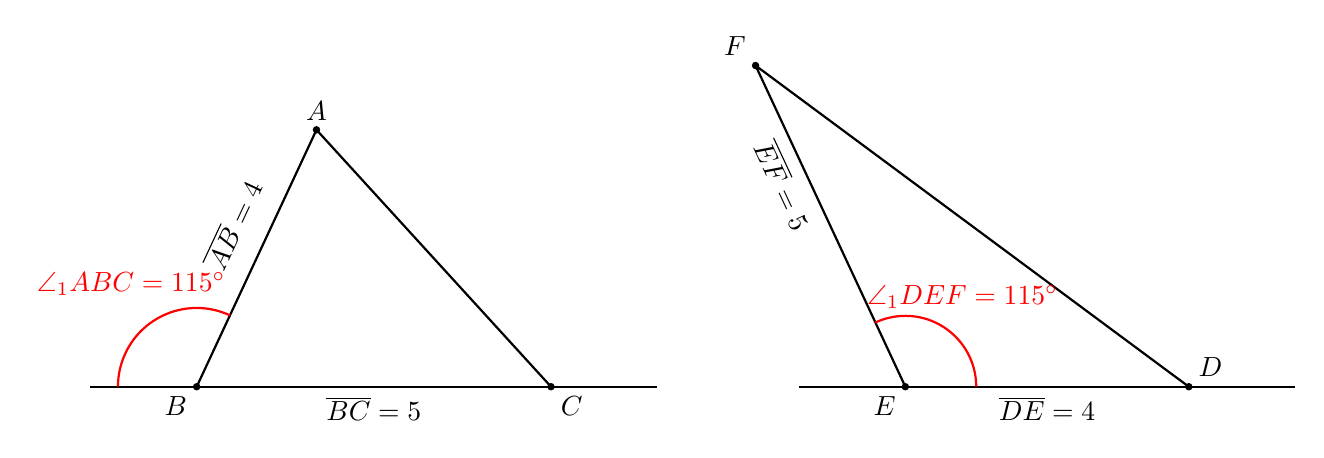
\begin{tikzpicture}[scale=.9, font=\sffamily]

    % ==========================================
    % TRIANGLE ABC (LEFT)
    % ==========================================
    % Define parameters
    \def\sideone{5}  % Length BC (L1)
    \def\sidetwo{4}  % Length AB (L2)
    \def\angleB{65}  % Inner angle of the triangle

    % Coordinates
    \coordinate (B) at (0,0);
    \coordinate (C) at (\sideone, 0);
    \coordinate (A) at (\angleB:\sidetwo);
    \coordinate (B_left) at (-1.5,0); % Point to define the leftward extension of line BC

    % Draw the extended line passing through B and C
    \draw[thick] (B_left) -- (\sideone + 1.5, 0);

    % Draw the other sides of the triangle
    \draw[thick] (B) -- (A) -- (C);

    % Plot points and label vertices
    \fill[black] (A) circle (1.5pt) node[above] {$A$};
    \fill[black] (B) circle (1.5pt) node[below left] {$B$};
    \fill[black] (C) circle (1.5pt) node[below right] {$C$};

    % Mark the 115 degree angle 
    % Increased eccentricity to 1.55 pushes the text higher
    \pic [draw, red, thick, angle eccentricity=1.55, angle radius=1cm, "$\angle_1 ABC = 115^\circ$"] {angle = A--B--B_left};

    % Label the given sides (black only)
    % Removed the downward y-shift to bring the label higher
    \node[below] at ($(B)!0.5!(C)$) {$\overline{BC} = 5$};
    
    % Adjusted the shift angle to 155 to move the label perfectly to the left of the slanted line
    \node[anchor=south, rotate=\angleB] at ($(A)!0.5!(B)+(100:0.35)$) {$\overline{AB} = 4$};


    % ==========================================
    % TRIANGLE DEF (RIGHT)
    % ==========================================
    \begin{scope}[xshift=10cm] % Shift the entire second drawing 10cm to the right
        % Define parameters
        \def\sideoneDEF{5}  % Length EF (L1)
        \def\sidetwoDEF{4}  % Length DE (L2)
        \def\angleE{115} % Inner angle of the triangle

        % Coordinates
        \coordinate (E) at (0,0);
        \coordinate (D) at (\sidetwoDEF, 0); % Set to (4,0) to be horizontal to the right
        \coordinate (F) at (\angleE:\sideoneDEF);
        \coordinate (E_left) at (-1.5,0); % Point to define the leftward extension of line DE

        % Draw the extended line passing through E and D
        \draw[thick] (E_left) -- (\sidetwoDEF + 1.5, 0);

        % Draw the other sides of the triangle
        \draw[thick] (E) -- (F) -- (D);

        % Plot points and label vertices
        \fill[black] (D) circle (1.5pt) node[above right] {$D$};
        \fill[black] (E) circle (1.5pt) node[below left] {$E$};
        \fill[black] (F) circle (1.5pt) node[above left] {$F$};

        % Mark the 115 degree interior angle 
        % Increased eccentricity to 1.55 pushes the text higher
        \pic [draw, red, thick, angle eccentricity=1.5, angle radius=.9cm, "$\angle_1 DEF = 115^\circ$"] {angle = D--E--F};

        % Label the given sides (black only)
        \node[below] at ($(E)!0.5!(D)$) {$\overline{DE} = 4$};
        
        % Shifted perpendicularly (115 + 90 = 205) to move the label perfectly left/above the slanted line
        % Note: rotate=-65 is used instead of 115 to prevent the text from being rendered upside-down
        \node[anchor=south, rotate=-65, left] at ($(E)!0.5!(F)+(205:0.35)$) {$\overline{EF} = 5$};
    \end{scope}
    \end{tikzpicture}
    \end{center}

    \begin{comment}
    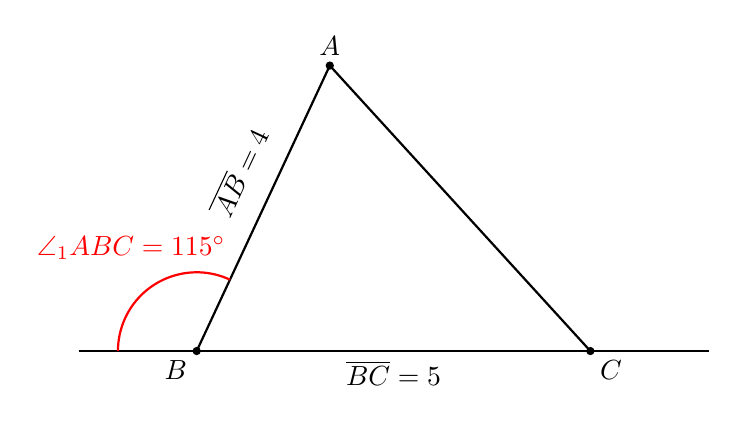
\begin{tikzpicture}[scale=1, font=\sffamily]

    % Define parameters
    \def\sideone{5}  % Length BC (L1)
    \def\sidetwo{4}  % Length AB (L2)
    \def\angleB{65}  % Inner angle of the triangle

    % Coordinates
    \coordinate (B) at (0,0);
    \coordinate (C) at (\sideone, 0);
    \coordinate (A) at (\angleB:\sidetwo);
    \coordinate (B_left) at (-1.5,0); % Point to define the leftward extension of line BC

    % Draw the extended line passing through B and C
    \draw[thick] (B_left) -- (\sideone + 1.5, 0);

    % Draw the other sides of the triangle
    \draw[thick] (B) -- (A) -- (C);

    % Plot points and label vertices
    \fill[black] (A) circle (1.5pt) node[above] {$A$};
    \fill[black] (B) circle (1.5pt) node[below left] {$B$};
    \fill[black] (C) circle (1.5pt) node[below right] {$C$};

    % Mark the 115 degree angle 
    % Increased eccentricity to 1.55 pushes the text higher
    \pic [draw, red, thick, angle eccentricity=1.55, angle radius=1cm, "$\angle_1 ABC = 115^\circ$"] {angle = A--B--B_left};

    % Label the given sides (black only)
    % Removed the downward y-shift to bring the label higher
    \node[below] at ($(B)!0.5!(C)$) {$\overline{BC} = 5$};
    
    % Adjusted the shift angle to 155 to move the label perfectly to the left of the slanted line
    \node[anchor=south, rotate=\angleB] at ($(A)!0.5!(B)+(100:0.35)$) {$\overline{AB} = 4$};

\end{tikzpicture}
    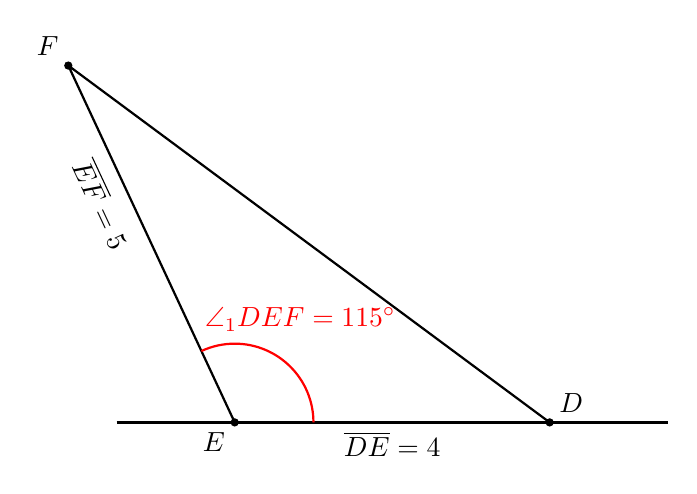
\begin{tikzpicture}[scale=1, font=\sffamily]

    % Define parameters
    \def\sideone{5}  % Length EF (L1)
    \def\sidetwo{4}  % Length DE (L2)
    \def\angleE{115} % Inner angle of the triangle

    % Coordinates
    \coordinate (E) at (0,0);
    \coordinate (D) at (\sidetwo, 0); % Set to (4,0) to be horizontal to the right
    \coordinate (F) at (\angleE:\sideone);
    \coordinate (E_left) at (-1.5,0); % Point to define the leftward extension of line DE

    % Draw the extended line passing through E and D
    \draw[thick] (E_left) -- (\sidetwo + 1.5, 0);

    % Draw the other sides of the triangle
    \draw[thick] (E) -- (F) -- (D);

    % Plot points and label vertices
    \fill[black] (D) circle (1.5pt) node[above right] {$D$};
    \fill[black] (E) circle (1.5pt) node[below left] {$E$};
    \fill[black] (F) circle (1.5pt) node[above left] {$F$};

    % Mark the 115 degree interior angle 
    % Increased eccentricity to 1.55 pushes the text higher
    \pic [draw, red, thick, angle eccentricity=1.55, angle radius=1cm, "$\angle_1 DEF = 115^\circ$"] {angle = D--E--F};

    % Label the given sides (black only)
    \node[below] at ($(E)!0.5!(D)$) {$\overline{DE} = 4$};
    
    % Shifted perpendicularly (115 + 90 = 205) to move the label perfectly left/above the slanted line
    % Note: rotate=-65 is used instead of 115 to prevent the text from being rendered upside-down
    \node[anchor=south, rotate=-65, left] at ($(E)!0.5!(F)+(205:0.35)$) {$\overline{EF} = 5$};
\end{tikzpicture}
    \end{comment}
    However, just by looking at these triangles it is clear that they are not congruent. The key difference between the two diagrams is the orientation of the points. We see that $ABC$ are oriented counter-clockwise while the points $DEF$ are oriented clock-wise. Thus, we must add a predicate \verb|sameclock A B C D E F| in order to track the orientations of points (in practice we can just read off the diagram the orientation of points). 
\end{example}

\begin{prop}[Euclid Book I Prop 4]\label{prop: Euclid Book 1 Prop 4 Angle 1} 
        If $AB = DE$, $BC = EF$, $\angle_1 ABC = \angle_1DEF$, and the
        orientation of the points $ABC$ are the same as that of $DEF$, then
        $\triangle ABC$ and $\triangle DEF$ are congruent.
\end{prop}

Thus, it seems that it might be the case where the \verb|sameclock| proposition is going to be the solution to any $\angle_1$ statements; however, we shall see in the next example that adding the \verb|sameclock| won't always be the fix to propositions. 

\begin{example}
    Consider Euclid Book I Prop 5, which is says in the $\angle_0$ case that: If $AB = AC$, then $\angle_0ABC = \angle_0ACB$. We might ask if it is the case, that this is still true with $\angle_1$ if we replace $\angle_0$ with $\angle_1$. However, it is clear that \verb|sameclock A B C A B C|. However, it is the case that $\angle_1 ABC \neq \angle_1 ACB$. We see this by drawing the diagram. 
    \begin{center}
    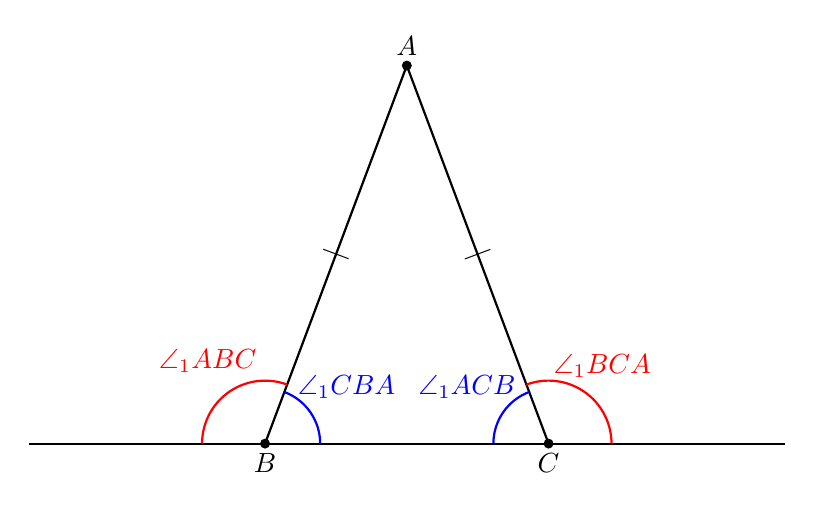
\begin{tikzpicture}[scale=1.2, font=\sffamily]

    % Coordinates for the isosceles triangle
    % Base vertices B and C are moved closer together (distance of 3 instead of 5)
    \coordinate (B) at (0,0);
    \coordinate (C) at (3,0);
    \coordinate (A) at (1.5, 4);
    
    % Coordinates to extend the BC line further out to the left and right
    \coordinate (B_left) at (-2.5,0);
    \coordinate (C_right) at (5.5,0);

    % Draw the extended base line
    \draw[thick] (B_left) -- (C_right);

    % Draw the slanted sides of the triangle
    \draw[thick] (A) -- (B);
    \draw[thick] (A) -- (C);

    % Plot points and label vertices
    \fill[black] (A) circle (1.5pt) node[above] {$A$};
    \fill[black] (B) circle (1.5pt) node[below] {$B$};
    \fill[black] (C) circle (1.5pt) node[below] {$C$};

    % Mark the angles
    
    % 1. Exterior angle at B (from AB to extended base on the left)
    \pic [draw, red, thick, angle eccentricity=1.6, angle radius=0.8cm, "$\angle_1 ABC$"] {angle = A--B--B_left};
    
    % 2. Interior angle at C (correctly located)
    \pic [draw, blue, thick, angle eccentricity=1.8, angle radius=0.7cm, "$\angle_1 ACB$"] {angle = A--C--B};

    \pic [draw, blue, thick, angle eccentricity=1.8, angle radius=0.7cm, "$\angle_1 CBA$"] {angle = C--B--A};

    
    % 3. Exterior angle at C (from extended base on the right to AC)
    \pic [draw, red, thick, angle eccentricity=1.5, angle radius=0.8cm, "$\angle_1 BCA$"] {angle = C_right--C--A};

    % Add tick marks to show AB = AC (Isosceles property)
    % Rotations are mathematically adjusted to ~69.4 degrees to perfectly match the steeper slope
    \node[rotate=69.4] at ($(B)!0.5!(A)$) {$|$};
    \node[rotate=-69.4] at ($(C)!0.5!(A)$) {$|$};
\end{tikzpicture}
    \end{center}
    Thus, we see that $\angle_1ABC \neq \angle_1 ACB$, but we have that
    $\angle_1ABC = \angle_1 BCA$ and $\angle_1ACB$ and $\angle_1CBA$.
    Furthermore, we can see that this is independent of the orientation of the
    points by drawing the other orientation of the picture.

    \begin{center}
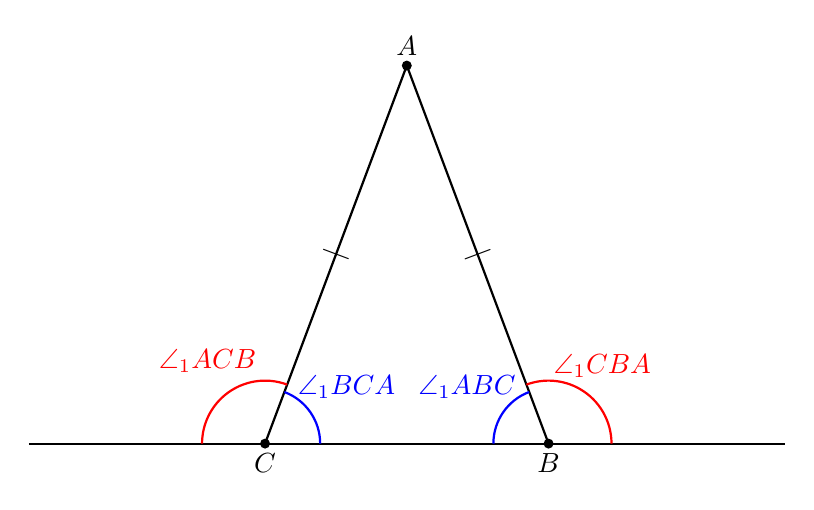
\begin{tikzpicture}[scale=1.2, font=\sffamily]

    % Coordinates for the isosceles triangle
    % B and C are swapped: C is now on the left (0,0) and B is on the right (3,0)
    \coordinate (C) at (0,0);
    \coordinate (B) at (3,0);
    \coordinate (A) at (1.5, 4);
    
    % Coordinates to extend the base line further out to the left and right
    \coordinate (C_left) at (-2.5,0);
    \coordinate (B_right) at (5.5,0);

    % Draw the extended base line
    \draw[thick] (C_left) -- (B_right);

    % Draw the slanted sides of the triangle
    \draw[thick] (A) -- (C);
    \draw[thick] (A) -- (B);

    % Plot points and label vertices
    \fill[black] (A) circle (1.5pt) node[above] {$A$};
    \fill[black] (C) circle (1.5pt) node[below] {$C$};
    \fill[black] (B) circle (1.5pt) node[below] {$B$};

    % Mark the angles
    
    % 1. Exterior angle at C (from AC to extended base on the left)
    \pic [draw, red, thick, angle eccentricity=1.6, angle radius=0.8cm, "$\angle_1 ACB$"] {angle = A--C--C_left};
    
    % 2. Interior angle at B (right side, previously at C)
    \pic [draw, blue, thick, angle eccentricity=1.8, angle radius=0.7cm, "$\angle_1 ABC$"] {angle = A--B--C};

    % 3. Interior angle at C (left side, previously at B)
    \pic [draw, blue, thick, angle eccentricity=1.8, angle radius=0.7cm, "$\angle_1 BCA$"] {angle = B--C--A};
    
    % 4. Exterior angle at B (from extended base on the right to AB)
    \pic [draw, red, thick, angle eccentricity=1.5, angle radius=0.8cm, "$\angle_1 CBA$"] {angle = B_right--B--A};

    % Add tick marks to show AC = AB (Isosceles property)
    % Note: Rotations are swapped to match the new side slopes
    \node[rotate=69.4] at ($(C)!0.5!(A)$) {$|$};
    \node[rotate=-69.4] at ($(B)!0.5!(A)$) {$|$};

\end{tikzpicture}
\end{center}
\end{example}

\begin{prop}[Euclid Book I Prop 5]\label{prop: Euclid Book 1 Prop 5 Angle 1}
    If $AB = AC$, then $\angle_1ABC = \angle_1BCA$. (We remark that $\angle_1ACB
    = \angle_1 CBA$ can be deduced from how $\angle_1$ works)
\end{prop}

\subsection{Angle between $x$-axis}\label{sec: d(AB)}

We shall now describe the computational short-cut that is needed, and will be
one the most powerful tool of AlphaGeometry to make it run fast. In particular,
we have defined $\angle_1$ between two lines. However, it will be more useful to
just give an angle for a single line. To do this, we shall consider the $x$-axis
as a reference point.

\begin{defn}
    For a line $AB$, we define the function $d(AB)$ to be the $\angle_1$ measure
    between the line $AB$ and the $x$-axis.
\end{defn}

\begin{center}
    \begin{tikzpicture}[scale=.8, font=\sffamily]

    % Define points for the x-axis
    \coordinate (X_left)  at (-1, 0);
    \coordinate (X_right) at (6, 0);

    % Define points for the line
    \coordinate (I) at (1, 0); % Intersection with x-axis
    \coordinate (A) at (2.5, 1.5);
    \coordinate (B) at (4.5, 3.5);
    
    % Points to extend the line visually in both directions
    \coordinate (Line_start) at (-0.5, -1.5);
    \coordinate (Line_end)   at (5.5, 4.5);

    % Draw x-axis
    \draw[thick] (X_left) -- (X_right) node[right, black] {$x$-axis};

    % Draw the arbitrary line AB passing through the x-axis
    \draw[thick] (Line_start) -- (Line_end);

    % Plot points A and B
    \fill[black] (A) circle (1.5pt) node[below right] {$A$};
    \fill[black] (B) circle (1.5pt) node[above left] {$B$};

    % Angle measurement: from line AB measured CCW to the x-axis
    % The order B--I--X_left draws the arc starting from ray IB towards the negative x-axis
    \pic [draw, red, thick, angle eccentricity=1.4, angle radius=1.0cm, "$d(AB)$"] {angle = B--I--X_left};

\end{tikzpicture}
\end{center}
We will discuss the importance of $d(AB)$ as it is more versatile when
implementing AR. Now we can see how to measure $\angle_1$ using $d$. In
particular, we have that $\angle_1ABC = d(AB)-d(BC).$

\begin{center}
    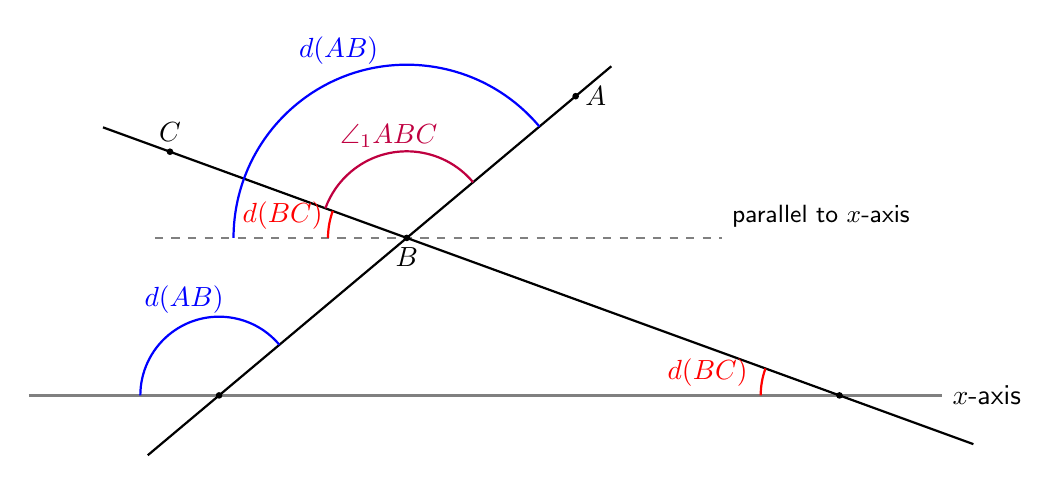
\begin{tikzpicture}[scale=.8, font=\sffamily]

    % ==========================================
    % DEFINE PARAMETERS & COORDINATES
    % ==========================================

    % Set base vector angles (angle from pos x-axis in coordinate system)
    \def\angleBA{40} % Ray BA angle (standard)
    \def\angleBC{160} % Ray BC angle (standard)
    \def\lenBA{3.5}
    \def\lenBC{4.0}

    % Define B at a specific off-axis coordinate
    \coordinate (B) at (2, 2.5);

    % Define A and C relative to B, using vector angles
    \coordinate (A) at ($(B) + (\angleBA:\lenBA)$);
    \coordinate (C) at ($(B) + (\angleBC:\lenBC)$);

    % Points for drawing reference lines parallel to the x-axis through B
    \coordinate (B_left)  at ($(B) + (-4, 0)$);
    \coordinate (B_right) at ($(B) + (5, 0)$);

    % Points for the main x-axis at the bottom
    % Extended X_left and X_right to comfortably encompass the intersection points
    \coordinate (X_left)  at (-4, 0);
    \coordinate (X_right) at (10.5, 0);

    % Calculate the exact intersection points of the lines with the x-axis
    \coordinate (I_AB) at (intersection of A--B and X_left--X_right);
    \coordinate (I_BC) at (intersection of C--B and X_left--X_right);

    % ==========================================
    % DRAW REFERENCE LINES & AXIS
    % ==========================================

    % Draw main gray x-axis at the bottom
    \draw[thick, gray] (X_left) -- (X_right) node[right, black] {$x$-axis};

    % Draw dashed gray line passing through B, parallel to the x-axis
    \draw[gray, thick, dashed] (B_left) -- (B_right) node[above right, black] {\small{parallel to $x$-axis}};

    % ==========================================
    % DRAW LINES AB & BC
    % ==========================================

    % Draw the lines extending past A and C, and past their x-axis intersections
    \draw[thick] ($(A)!-0.1!(I_AB)$) -- ($(I_AB)!-0.2!(A)$);
    \draw[thick] ($(C)!-0.1!(I_BC)$) -- ($(I_BC)!-0.2!(C)$);

    % Draw visual indicators for A and C points
    \fill[black] (A) circle (1.5pt) node[right] {$A$};
    \fill[black] (C) circle (1.5pt) node[above] {$C$};

    % Draw visual indicator for B point at intersection
    \fill[black] (B) circle (1.5pt) node[below] {$B$};

    % Draw visual indicators for the x-axis intersection points
    \fill[black] (I_AB) circle (1.5pt);
    \fill[black] (I_BC) circle (1.5pt);

    % ==========================================
    % MARK THE ANGLES
    % ==========================================

    % --- Angles at vertex B ---
    % 1. d(AB) at B: Angle from Line AB CCW to the parallel x-axis
    \pic [draw, blue, thick, pic text options={yshift=-0.35cm}, angle eccentricity=1.15, angle radius=2.2cm, "$d(AB)$"] {angle = A--B--B_left};

    % 2. d(BC) at B: Angle from Line BC CCW to the parallel x-axis
    \pic [draw, red, thick, angle eccentricity=1.6, angle radius=1cm, "$d(BC)$"] {angle = C--B--B_left};

    % 3. Angle_1 ABC at B: Direct angle from Ray BA to Ray BC CCW
    \pic [draw, purple, thick, angle eccentricity=1.2, angle radius=1.1cm, "$\angle_1 ABC$"] {angle = A--B--C};

    % --- Angles at the x-axis intersections ---
    % 4. d(AB) at x-axis: Angle from Line AB CCW to the x-axis
    \pic [draw, blue, thick, pic text options={yshift=-0.35cm}, angle eccentricity=1.3, angle radius=1.cm, "$d(AB)$"] {angle = A--I_AB--X_left};

    % 5. d(BC) at x-axis: Angle from Line BC CCW to the x-axis
    \pic [draw, red, thick, angle eccentricity=1.7, angle radius=1cm, "$d(BC)$"] {angle = C--I_BC--X_left};

\end{tikzpicture}
\end{center}

If we consider this picture, it is clear that we get $\angle_1 ABC =
d(AB)-d(BC)$; however, we must again be careful that our picture is not
misleading us. Thus, let us consider the same diagram, but switch the locations
of $A$ and $C$.

\begin{center}
    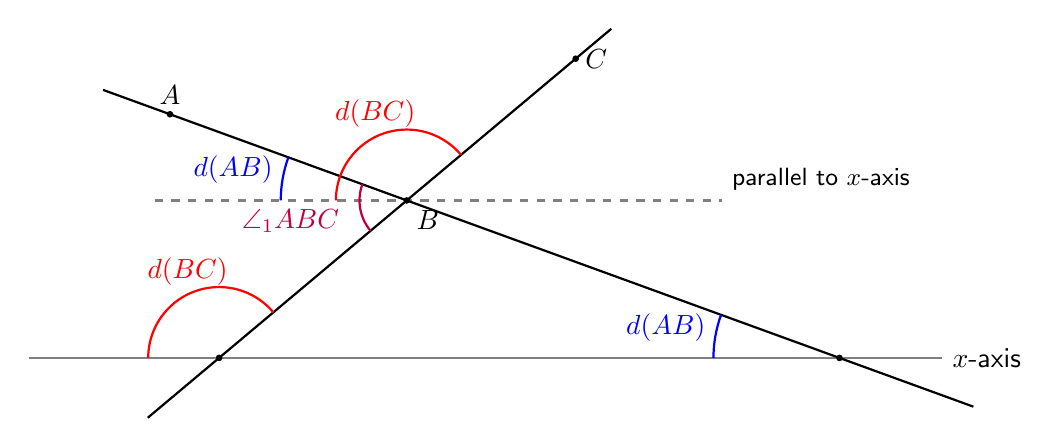
\begin{tikzpicture}[scale=.8, font=\sffamily]

    % ==========================================
    % DEFINE PARAMETERS & COORDINATES
    % ==========================================

    % SWAPPED base vector angles and lengths
    \def\angleBA{160} % Ray BA angle (now pointing top-left)
    \def\angleBC{40}  % Ray BC angle (now pointing top-right)
    \def\lenBA{4.0}
    \def\lenBC{3.5}

    % Define B at a specific off-axis coordinate
    \coordinate (B) at (2, 2.5);

    % Define A and C relative to B, using vector angles
    \coordinate (A) at ($(B) + (\angleBA:\lenBA)$);
    \coordinate (C) at ($(B) + (\angleBC:\lenBC)$);

    % Points for drawing reference lines parallel to the x-axis through B
    \coordinate (B_left)  at ($(B) + (-4, 0)$);
    \coordinate (B_right) at ($(B) + (5, 0)$);

    % Points for the main x-axis at the bottom
    \coordinate (X_left)  at (-4, 0);
    \coordinate (X_right) at (10.5, 0);

    % Calculate the exact intersection points of the lines with the x-axis
    \coordinate (I_AB) at (intersection of A--B and X_left--X_right);
    \coordinate (I_BC) at (intersection of C--B and X_left--X_right);

    % ==========================================
    % DRAW REFERENCE LINES & AXIS
    % ==========================================

    % Draw main gray x-axis at the bottom
    \draw[thick, gray] (X_left) -- (X_right) node[right, black] {$x$-axis};

    % Draw dashed gray line passing through B, parallel to the x-axis
    \draw[gray, thick, dashed] (B_left) -- (B_right) node[above right, black] {\small{parallel to $x$-axis}};

    % ==========================================
    % DRAW LINES AB & BC
    % ==========================================

    % Draw the lines extending past A and C, and past their x-axis intersections
    \draw[thick] ($(A)!-0.1!(I_AB)$) -- ($(I_AB)!-0.2!(A)$);
    \draw[thick] ($(C)!-0.1!(I_BC)$) -- ($(I_BC)!-0.2!(C)$);

    % Draw visual indicators for A and C points (adjusted label positions for new locations)
    \fill[black] (A) circle (1.5pt) node[above] {$A$};
    \fill[black] (C) circle (1.5pt) node[right] {$C$};

    % Draw visual indicator for B point at intersection
    \fill[black] (B) circle (1.5pt) node[below right] {$B$};

    % Draw visual indicators for the x-axis intersection points
    \fill[black] (I_AB) circle (1.5pt);
    \fill[black] (I_BC) circle (1.5pt);

    % ==========================================
    % MARK THE ANGLES
    % ==========================================

    % --- Angles at vertex B ---
    % 1. d(AB) at B: Angle from Line AB CCW to the parallel x-axis
    % Adjusted to a smaller radius since the angle is now only 20 degrees
    \pic [draw, blue, thick, angle eccentricity=1.4, angle radius=1.6cm, "$d(AB)$"] {angle = A--B--B_left};

    % 2. d(BC) at B: Angle from Line BC CCW to the parallel x-axis
    % Adjusted radius for the wider 140 degree angle
    \pic [draw, red, thick, angle eccentricity=1.3, angle radius=0.9cm, "$d(BC)$"] {angle = C--B--B_left};

    % 3. Angle_1 ABC at B: Direct angle from Ray BA to Ray BC CCW
    % This is now a reflex angle (240 degrees), pushed closer to the vertex to avoid line overlap
    \pic [draw, purple, thick, angle eccentricity=2.5, angle radius=0.6cm, "$\angle_1 ABC$"] {angle = A--B--I_BC};

    % --- Angles at the x-axis intersections ---
    % 4. d(AB) at x-axis: Angle from Line AB CCW to the x-axis
    \pic [draw, blue, thick, angle eccentricity=1.4, angle radius=1.6cm, "$d(AB)$"] {angle = A--I_AB--X_left};

    % 5. d(BC) at x-axis: Angle from Line BC CCW to the x-axis
    \pic [draw, red, thick, angle eccentricity=1.3, angle radius=0.9cm, "$d(BC)$"] {angle = C--I_BC--X_left};

\end{tikzpicture}
\end{center}

In this picture, we now see the subtlety. In particular, we have that
$d(AB)-d(BC)$ will be negative. Furthermore, the angle measurement $\vert
d(AB)-d(BC)\vert$ is not $\angle_1 ABC$, so we simply cannot take absolute
value. However, we see that
\[
\angle_1(ABC) + d(BC) -d(AB) = 180\degree.
\]
Thus, we will have that 
\[
\angle_1 ABC\equiv d(AB) -d(BC) \pmod{ 180\degree}.
\]
This is why we must consider the angle modulo $180\degree$, and have that
$\angle_1 ABC $ is measured modulo $180\degree$.

\section{Basic Geometric Objects}\label{sec: Basic Geometric Objects}

In this section, we will discuss the basic geometric objects that we will store in the system. In practice, we could create our entire system only using \textbf{points} and building our predicates out of these points. However, in practice when solving geometry, we look at diagrams, and by looking at the diagrams, we can then reason and make conjectures. For our AI, this amounts to looking at the different objects which are present in the diagram, and then by hashing them, we can make conjectures that may be true based off our diagram. Thus, we will only try to prove things which might be true since if in our diagram there is two angles aren't equal, we shouldn't try to prove that they are and therefore waste time computing. Each of these should be made their own \verb|class| in the \verb|geometry.py| file. 

\subsection{Points}\label{subsec: Points}
A \textbf{point} is the most basic geometric object. Since all predicates are built in terms of points, when implementing our system we shall build a \verb|Point| class. These should have the following data associated to the \verb|Point|
\begin{itemize}
    \item \verb|x| this will be a float that represents the $x$-coordinate of the point. To determine this point we read it off the diagram of the problem. 
    \item \verb|y| this will be a float that represents the $y$-coordinate of the point.
    \item \verb|name| This is a string that is just the name of the point. 
    \item \verb|constructed| This will be a boolean that tells us if the point was constructed during the problem. 
    \item \verb|index| (this is just a global index for when this point was created to )
    \item \verb|depth| this is a marker to denote in what order that the point was constructed. A point given in the statement of the problem should have depth $0$. Points created after the first construction call should have depth $1$, and so on.
    \item \verb|overlaps| this is a boolean that checks to see if this point overlaps with another point
\end{itemize}
Combinatorially, we shall assume that we have $n$ points in our problem (of
course this number will grow), but we will measure all the other number of
geometric objects in terms of the number of points.

\subsection{Lines}\label{subsec: Lines}

The idea behind the lines, is that of collinearity, in particular, when do
points lie on the same line. In particular, we shall

Thus, you should create a \verb|Line| class, and associated to the line, there should be the following data
\begin{itemize}
    \item \verb|equation| this will be the equation of the line, when creating a point, we should check to see which lines it falls upon
    \item \verb|points| this will be the set of points that lie on this line
    \item \verb|name| this will be the name of this line
    \item \verb|constructed| this is a boolean that will denote whether or not this line was constructed or given from the statement of the problem
    \item \verb|index| this is a global index for this line 
    \item \verb|depth| this is a marker to denote in what order this line was created
    
\end{itemize}

Combinatorially, the worst case scenario will occur if no three points are
collinear. Thus, every two points will form a line; thus, there will be
$\binom{n}{2} = O(n^2)$ lines.

\subsection{Segments}\label{subsec: Segments}

The idea behind segments is the same as lines; however, we use the segments to
measure the distance between two points, so we will create a segment for every
pair of points.

Thus, you should create a \verb|Segment| class. These should have the following data associated to them
\begin{itemize}
    \item \verb|name| this is just the name of the segment
    \item \verb|points| this will have the two points that determine the segment
    \item \verb|length| this is the numeric quantity of the length of the segment (we shall use this as a hash to conjecture possible \verb|cong| relations)
    \item \verb|index| this is a global index for this segment (we shall use these segments and these indices in AR)
    \item \verb|constructed| this is a boolean 
    \item \verb|depth| this a marker to denothe in what order this segment was created
\end{itemize}


Combinatorially, we have that every two distinct points determines a segment, so
we will have $\binom{n}{2}=O(n^2)$ points.

\subsection{Pairs of Segments} Once we have segments, there will be times where we wish to look at the ratio between two segments. Such computations are useful when determining the \verb|eqratio| or \verb|rcompute| predicate. Now instead of computing all the ratios at all times. We can precompute the ratios between two segments, and then if we hash these pairs by the numeric value of the ratio, then when creating new pairs of ratios, we can check to see if the hash values match 

\subsection{Circles}\label{subsec: Circles}
There are two ideas behind that of circles, namely \verb|circle O A B C| which denotes circumcircles, and \verb|cyclic A B C D| which denotes points lying on the same circle. The downside is that \verb|cyclic| may doesn't capture the center of the circle, so there is also the variant of \verb|cyclic_with_center| which captures the center. 

\subsection{Angles}\label{subsec: Angles}

\subsection{Triangles}\label{subsec: triangles}


\textcolor{red}{FINISH WRITNG THE REMAINDER OF THE GEOMETRIC OBJECTS}

\section{Basic Predicates}

In this section, we will discuss the basic predicates that we will use in our geometry system, and how we will choose to store this data. The general outline is as follows: our system will use predicates of the form \verb|col A B C|, \verb|eqangle A B C P Q R|, \verb|cong A B C D|, etc.. In the above, each of the terms \verb|col|, \verb|eqangle|, and \verb|cong| are \textbf{predicates} that correspond to some geometric property in this case collinear points, equality of angles, and congruence of segments respectively. While \verb|A B C D P Q R| all represent \textbf{points} in the problem statement. There are a few predicates which also involve other variables, but we will discuss those as they come up. Thus, a predicate consists of some word that signifies the geometric relation followed by some points. The word will signify the relation that the points satisfy. 

We remark that we build everything based off of the points of the problem, and
the points will be the geometric objects that we consider when dealing with
predicates. While it may be possible to have predicates that take in other
geometric objects such as lines, triangles, circles, etc., including such
information in the predicates might complicate things. Thus, we build everything
off of points; however, our other geometric objects are used for generating
conjectures.


Once we have points, we can start putting them together into predicates such as \verb|col A B C|. We shall make a class for each of the different kinds of predicates. However, there are a lot of shared attributes of each kind of predicate. Thus, we shall create a class called \verb|RelationNode| which is the abstraction of all the different kinds of predicates. Furthermore, each \verb|RelationNode| can be thought of as the vertex in the proof graph.

The \verb|RelationNode| class should have the following data associated to it:
\begin{itemize}
    \item \verb|name| this will be the name of the node
    \item \verb|type| this tells us what predicate the node should be.
    \item \verb|index| this should be 
    \item \verb|given| this is a Boolean which is true if the predicate was given in the problem statement, and false if it was deduced
    \item \verb|parents| this will be a list of other predicates where if the given node was deduced from other information then the parents describe the geometric information used in deducing the given predicate
    \item \verb|rule| this will be a string which says by which rule (or if AR was used) in the deduction
    \item \verb|statement| this will be a string used when outputting the proof that will state how the relation is known. Whether it is given, deduced in DD (from which rule and what the parents were), or deduce from AR (explaining the linear combination used in the deduction). 
\end{itemize}

The proof graph will be a directed graph whose vertices correspond to \verb|RelationNode|s, and whose edges correspond to the \verb|parents| of the given nodes. Thus, the \verb|parents| data should be considered as directed edges for a given node pointing to where it came from. Using this structure, we have that 
\textcolor{red}{FIGURE OUT WRITING THE REST OF THIS}

\subsection{coll}

\subsection{cong}

\subsection{cyclic}

\subsection{cyclic\_with\_center}

\subsection{circle}

\subsection{eqangle}

\subsection{para}

\subsection{perp}

\subsection{midp}

\subsection{eqratio}

\subsection{simtri1(2)}

\subsection{contri1(2)}

\subsection{acompute}

\subsection{rcompute}

\subsection{distmeq}

\subsection{distseq}

\subsection{angeq}

\subsection{sameclock}

\subsection{sameside}

\subsection{overlap}


\section{Problem Data Structure}

Now we will discuss the Problem Data Structure. This will be the contents of the \verb|Problem.py| file. In particular, this 

\section{Deductive Database}

Now the \textbf{Deductive Database (DD)} is one of the more basic ideas of
AlphaGeometry. The general idea of DD is that it is a list of rules where we.

\section{Generating Conjectures}

\section{Algebraic Reasoning}

\subsection{Angle Matrix}

\subsubsection{Measure of a Line with Respect to the $x$-axis}
In this section, we discuss a different way to calculate $\angle_1$. This is not
a different angle convention, but rather a way that w

\subsection{Ratio Matrix}

\section{The Basic Solver}\label{sec: Basic Solver}
At this point, we have now developed a basic geometry solver. The loop and
algorithm to solve this

\section{Implementing Area}

We shall now discuss the issue of area. The classical versions of AlphaGeometry
and AlphaGeometry2 do not consider the concept of area. In doing so, these
systems can't deduce the Pythagorean theorem. In this section, we will discuss
what additions and complications come up when trying to define area.

For the highly motivated students, you may try to implement the concept of area
into your system (consider it an extra-credit project or a challenge for those
who are interested).

\subsection{Area Matrix}

\section{Auxiliary Constructions}

The goal of this section is to discuss the various kind of rabbits that we might consider. We shall create a file called \verb|constructions.py| which will do these geometric constructions and .

\section{Generating Synthetic Data}
Now that we have a basic solver, and a way to do constructions. The goal now is
to come up with data that will then be used to

\section{Cleaning the Data}\label{sec: Cleaning the data}

In this section, we will briefly discuss the process of cleaning the synthetic data. In particular, it might be the case that when generating the synthetic data, you may have two data points which appear to be different, but are actually the same. What we mean by this is that the two data points might have for example \verb|col A B C| and \verb|col X Y Z| in the assumptions, and after doing the transformation $A\mapsto X$, $B\mapsto Y$, and $C\mapsto Z$, then the two data points may actually be the same. 

Another way in which two data points might look different, but are actually the same, is that the predicates might appear in a different order. That is \verb|col A B C; col C D E...| should be the same as \verb|col C D E; col A B C...|

Thus, for the synthetic data, even though the points that appear
\textcolor{red}{FINISH WRITING THIS}


\section{Fine Tuning the Language Model}\label{sec: Fine Tuning the Language
Model}

In the original run of this course, we had an engineer from Google DeepMind give a guest lecture on fine-tuning the language model. In particular, we had used \href{https://ai.google.dev/gemma/docs/tune}{Gemma (documentation linked here)} as the language model in which we had finetuned. For those who have more experience with language models and want to explore/experiment with others, feel free to use \href{https://huggingface.co/}{Hugging Face}. 

In particular, the hardest part of fine-tuning the language model was just coming up with the data to tune the model on. Once, you have the data, then fine tuning is as simple as following a tutorial such as this one for \href{https://gemma-llm.readthedocs.io/en/latest/colab_finetuning.html}{Gemma (tutorial linked)}.

For those at Brown, we recommend doing the finetuning on OSCAR (Brown's super
computer).

\section{$n$-Shot Prompting}\label{sec: n-shot prompting}

An alternative to fine-tuning a language model which also can solve the problem,
is the idea of prompt engineering, and $n$-shot prompting. The benefit to
$n$-shot prompting is that it requires a smaller amount of synthetic data, and
it is easier to change which language model you use (without having to fine-tune
another model).

For $n$-shot prompting, you will write a preset prompt to give the language
model (which will only change with the given problem). In addition, you will
also give the language model $n$ examples of input/output pairs from your
synthetic data, then the language model will give its guess to the correct
output.

One advantage that this has is that you may feed the language model more context
(such as a natural language statement); however, we remark that this strategy
has the downside is that you are feeding the language model a larger prompt, so
it will require more tokens to run compared to a fine-tuned model where you just
feed in the formalization.

Here is a rough outline of what a prompt may look like:

``
You are a Euclidean geometry expert that solved IMO geometry problems. You must give a geometric construction that is useful in solving the following geometry problem \verb|{natural language statement}|.

We use the following system to formalize the problem... (here you will give an
explanation of the predicates and their meanings)

Furthermore, you may suggest the following constructions... (here you will give
a description of the constructions in your system)

We have currently done the following constructions; thus far \verb|{constructions perfomred}|.

A formalized version of the current state of the problem after finding all possible deductions is given by \verb|{Formal State of the Problem}|.

Here is an example of $n$ examples of input problem states, and output construction suggestions that have worked for previous problems \verb|{List of n Examples}|. 

Give the construction in the required output format. 
''

\bigskip
Once you have your prompt, you can just incorporate this LLM call into the main
loop of your solver when you get stuck to suggest a construction.

\section{Integrating the Language Model}\label{sec: Integrating the language
model}

Now that we have discussed the way in which we can use language models to help
solve our math problems, we can now integrate them into the solving loop. In
particular, you might consider having different modes for your system to run on.

\begin{enumerate}
    \item Basic Mode: This is the mode as described in \Cref{sec: Basic Solver}
          where you just run your deduction system to see if it solves the
          problem.

    \item Random Construction Mode: This mode will run the Basic solver until
          either it can't deduce anything more, or it has gone through enough
          loops of the deduction system. At that point, a random construction
          will be applied, and new conjectures will be formed, and then the
          basic solver will be run again (until a threshold of a given number of
          random constructions are done), or if the problem is solved.

    \item Expert Mode: This mode is like random; however, rather than applying a
          random construction. It will specifically apply constructions that are
          related to a given triangle (i.e. for a given triangle construct its
          circumcenter, orthocenter, excenters, etc.). The idea is that these
          points are useful for a triangle to argue around, so just do them all
          for a triangle, and hopefully this will do better than just a random
          construction.

    \item Fine-tuned Mode: This mode will prompt the fine-tuned language model
          if it is unable to deduce the goal.

    \item $n$-Shot Prompting Mode: This mode will prompt the language model
          using the idea of prompt engineering and $n$-shot prompting.

\end{enumerate}

\section{Automatic Diagram Generation and Autoformalization}
This brief section is about incorporating an automatic diagram generation and/or
autoformalization into your system. In the initial run of the course, we did not
include this material. However, we shall include a section for students who wish
to incorporate it (or part of it) into their systems. In particular, rather than
building a diagram generator from scratch, each team may search for some
automatic diagram generators of that currently exist. We shall detail the pros
and cons of incorporating this into your system, and a few automatic diagram
generators that currently exist

\textbf{Pros:}
\begin{itemize}
    \item Automatic diagram generation and autoformalization will allow for a
          single pipeline where you will input a natural language statement and
          then the system will produce a proof
    \item Simpler for the user of the system
    \item You can generate multiple diagrams, and if the system proves the
          result, that helps insure that the proof need not rely on the diagram
\end{itemize}

\textbf{Cons:} 
\begin{itemize}
    \item The autoformalized or generated diagram may be incorrect leading to
          the system having issues solving the problem
    \item We have built our system based off reading in a geogebra \verb|.ggb| file and scrapping this data, to incorporate this there may be a different structure that you will need to learn and then write code to integrate it into your system
    \item If the autoformalizer hallucinates it may either lead out a predicate
          that is needed to solve the problem, or add an additional predicate
          which is not necessarily given, but makes the problem trivial.
\end{itemize}

For automatic diagram generation, you may consider \cite{krueger2021automatically} which has a github \hyperlink{https://github.com/rkruegs123/geo-model-builder}{(click here to access)} that you may integrate into your system. However, if there are other automatic diagram generators that you wish to find and use, feel free to use those. 

For autoformalization, you may try to use a language model in which you could
try to do $n$-shot prompting with examples (since there isn't enough data to
fine tune a model), you could also try doing a loop with agents in which you
have several LLMs, one formalizes, and then one checks the formalization, and
then you can have an editor. This loop will decrease the chance of
hallucination.


%\textcolor{red}{FINISH WRITING THIS basically cite the thingy and then talk
%about how there might be issues generating a diagram from natural language.
%Thus, they might have a few different ``main'' things depending on what they
%want to input into their system. } \cite{krueger2021automatically}

\section{Power of a Point}
For the remainder of the notes (until we present the coding homeworks at the end
of the document), we shall present some of the tools/theorems in Euclidean
geometry. These concepts might not be used in your system, but you could try to
either build your system in such a robust way that you can prove these theorems,
or you could try to incorporate some of these theorems in your DDAR (although
that might be a bit tricky).

We begin this section by discussing the \textbf{power of a point} which is a
quantity that relates a point $P$ and a given circle.

\begin{defn}
    The \textbf{power of a point} $P$ with respect to a circle with center $O$
    and radius $OA$ is the quantity:
    \[
    \Pi(P)=PO^2 - OA^2.
    \]
\end{defn}

We remark that, even though our definition of the power of a point involves the point $A$. 
Since we just have the quantity $OA^2$ which is the radius of the circle squared. 
This quantity is independent of the point $A$ chosen on the circle. 
In particular, it is most useful to pick a point $A$ such that \verb|perp P A A O|. 
Thus, we will have a right triangle, and can use the Pythagorean theorem. 
Thus, the power of a point $P$ is the square of the distance of the tangent segement from $P$ to the circle.  
\vspace{10pt}
\begin{center}
    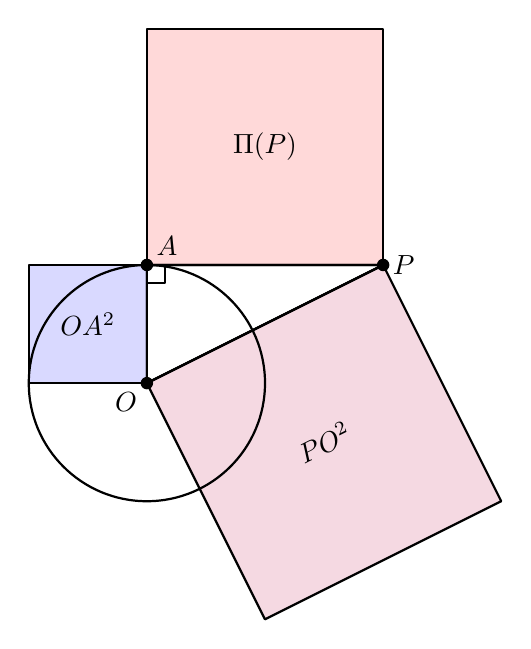
\begin{tikzpicture}[scale=1.5, font=\sffamily, line join=round]

    % Define main coordinates
    \coordinate (O) at (0,0);
    \coordinate (A) at (0,1);
    \coordinate (P) at (2,1);

    % ==========================================
    % DRAW PYTHAGOREAN SQUARES
    % ==========================================
    
    % Square on OA (Radius squared)
    % Vertices go leftwards from the y-axis to sit outside the triangle
    % Side length is 1 unit. Correct.
    \draw[thick, fill=blue!15] (0,0) -- (-1,0) -- (-1,1) -- (0,1) -- cycle;
    \node at (-0.5, 0.5) {$OA^2$};

    % --- CORRECTED ---
    % Square on AP (Power of the point / Tangent squared)
    % Vertices go upwards to sit outside the triangle
    % The length of AP is 2 units. 
    % We must draw the square from y=1 up to y=3 to get a side length of 2.
    \draw[thick, fill=red!15] (0,1) -- (0,3) -- (2,3) -- (2,1) -- cycle;
    \node at (1, 2) {$\Pi(P)$}; % Moved label center for the taller box

    % Square on OP (Distance to center squared)
    % Vertices calculated using the perpendicular vector (1, -2) to sit outside
    \draw[thick, fill=purple!15] (0,0) -- (1,-2) -- (3,-1) -- (2,1) -- cycle;
    % Rotated the text to align perfectly with the hypotenuse OP
    \node[rotate=26.56] at (1.5, -0.5) {$PO^2$}; 

    % ==========================================
    % DRAW CIRCLE AND TRIANGLE
    % ==========================================

    % Draw the circle (radius 1)
    \draw[thick] (O) circle (1);

    % Draw the main right triangle PAO with a white background to stand out
    \draw[thick] (O) -- (A) -- (P) -- cycle;
    \draw[thick] (O) -- (A) -- (P) -- cycle; % Redraw borders so they are sharp

    % ==========================================
    % LABELS AND MARKERS
    % ==========================================

    % Right angle marker at vertex A (where tangent meets radius)
    \draw[thick] (0, 0.85) -- (0.15, 0.85) -- (0.15, 1);

    % Draw points and label them
    \fill[black] (O) circle (1.5pt) node[below left] {$O$};
    \fill[black] (A) circle (1.5pt) node[above right] {$A$};
    \fill[black] (P) circle (1.5pt) node[right] {$P$};

\end{tikzpicture}
\end{center}


However, we now see an issue with this visualization of the power of a point. In
particular, it depended upon the point $P$ being located outside of the circle.
Since a point inside the circle will not have a tangent to the circle. 
The definition allows for points inside of the circle. We see
that
\[
\Pi(P):\begin{cases}
    >0 & \text{P is outside the circle}\\
    <0 & \text{P is inside the circle}\\
    =0&\text{$P$ is on the circle}
\end{cases}
\]

However, if $P$ is inside the circle, then we can not pick a point $A$ so that \verb|perp P A A O|. 
To get around this, we can still make a right triangle, but picking $A$ so that \verb|perp O P P A|. 
Then we will have that $\Pi(P)$ is the negative area of the corresponding square. 
In particular, we can visualize this in the figure below.

\vspace{10pt}
\begin{center}
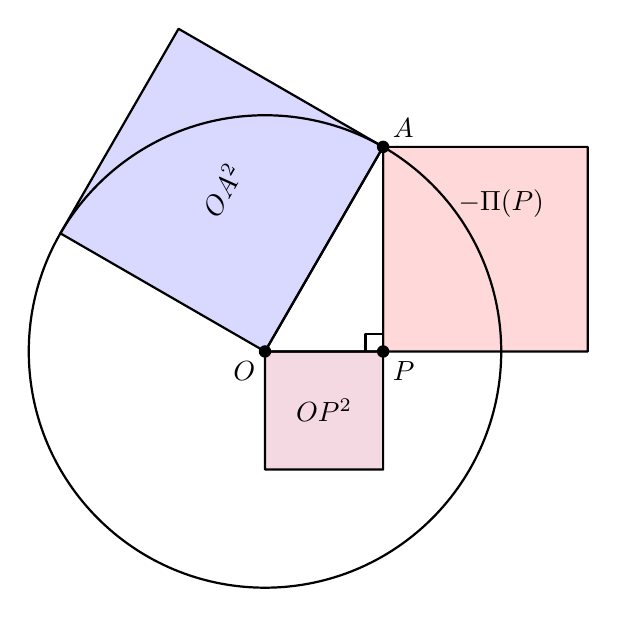
\begin{tikzpicture}[scale=1.5, font=\sffamily, line join=round]

    % P inside the circle: O at origin, circle of radius 2, P at (1,0) inside.
    % Pick A on the circle so that perp O P P A, i.e. right angle at P.
    % Since OP is horizontal, PA is vertical, giving A at (1, sqrt(3)).
    \coordinate (O) at (0,0);
    \coordinate (P) at (1,0);
    \coordinate (A) at (1,{sqrt(3)});

    % ==========================================
    % DRAW PYTHAGOREAN SQUARES
    % ==========================================

    % Square on OP (shorter leg, going downward)
    \draw[thick, fill=purple!15] (O) -- (P) -- (1,-1) -- (0,-1) -- cycle;
    \node at (0.5,-0.5) {$OP^2$};

    % Square on PA = -Pi(P) (longer leg, going to the right)
    \draw[thick, fill=red!15] (P) -- (A) -- ({1+sqrt(3)},{sqrt(3)}) -- ({1+sqrt(3)},0) -- cycle;
    \node at ({2},{1.25}) {$-\Pi(P)$};
    %\node at ({1+sqrt(3)/2},{sqrt(3)/2}) {$-\Pi(P)$};

    % Square on OA (hypotenuse, going upper-left away from triangle interior)
    % Perpendicular to OA rotated 90 CCW from direction (1,sqrt(3)) is (-sqrt(3),1)
    \draw[thick, fill=blue!15] (O) -- ({-sqrt(3)},1) -- ({1-sqrt(3)},{1+sqrt(3)}) -- (A) -- cycle;
    \node[rotate=60] at ({(1-sqrt(3))/2},{(1+sqrt(3))/2}) {$OA^2$};

    % ==========================================
    % DRAW CIRCLE AND TRIANGLE
    % ==========================================

    \draw[thick] (O) circle (2);
    \draw[thick] (O) -- (P) -- (A) -- cycle;

    % ==========================================
    % LABELS AND MARKERS
    % ==========================================

    % Right angle marker at P (between OP going left and PA going up)
    \draw[thick] (0.85,0) -- (0.85,0.15) -- (1,0.15);

    \fill[black] (O) circle (1.5pt) node[below left] {$O$};
    \fill[black] (P) circle (1.5pt) node[below right] {$P$};
    \fill[black] (A) circle (1.5pt) node[above right] {$A$};

\end{tikzpicture}
\end{center}
\vspace{10pt}

We remark that due to its complex nature of involving a point, the center, and
radius of a circle as well as its definition involving the non-linear operation
of squaring. It isn't clear how to incorporate such a quantity in your AI.
Furthermore, it is unclear what this quantity is actually measuring just from
its definition. We now discuss a theorem that describes the power of point 
with respect to a circle to a ratio between either the secant line (in the case
that the point is outside the circle), or the chord containing the point (in
the case that the point lies inside the circle).

We remark that the statement of the theorem is different in the fact that the
assumption lie in the angle part of AR while the conclusion lies in the ratio 
part of AR. Furthermore, as this is an implication rather than an if and only if
statement, such a rule might be more appropriate for DD if you wish to implement
it.

\begin{prop}
\verb|perp P A A O; cong O A O B; cong O A O C; col P B C|$ \Rightarrow$ \verb|PA^2 = P B| $\cdot$ \verb|PC|.

In particular, we see that as $PA^2 = \vert \Pi(P)\vert^2$, we can state the conclusion of the theorem as $\Pi(P) = PB \cdot PC$.
In this case, we need not even have reference to the point $A$ in the theorem statement. 

For $P$ outside the circle, this is the so called tangent-secant theorem. 

For $P$ inside the circle, this is the so called intersecting chords theorem. 
\end{prop}

\begin{proof}
We consider the case where $P$ is outside the circle. Draw the radii $OA$, $OB$, $OC$ and the triangle $ABC$, as illustrated below.

\begin{center}
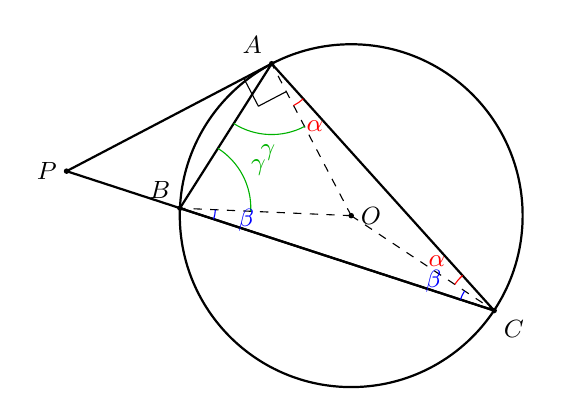
\begin{tikzpicture}[scale=0.5, font=\small\sffamily, line join=round]

    % Coordinates derived from Geogebra:
    % O=(0,0), B=(-4.35,0.19), P=(-7.23,1.13), circle radius ~4.354
    % A = upper tangent point from P, C = second intersection of line PB with circle
    \coordinate (O) at (0, 0);
    \coordinate (B) at (-4.35, 0.19);
    \coordinate (P) at (-7.23, 1.13);
    \coordinate (A) at (-2.02, 3.86);
    \coordinate (C) at (3.63, -2.41);

    % Circle, tangent PA, and secant PBC
    \draw[thick] (O) circle (4.354);
    \draw[thick] (P) -- (A);
    \draw[thick] (P) -- (C);

    % Triangle ABC
    \draw[thick] (A) -- (B) -- (C) -- cycle;

    % Radii OA, OB, OC (dashed)
    \draw[dashed] (O) -- (A);
    \draw[dashed] (O) -- (B);
    \draw[dashed] (O) -- (C);

    % Right angle marker at A (tangent perp to radius)
    \pic [draw, angle radius=0.4cm] {right angle = O--A--P};

    % gamma (green): base angles of isosceles triangle OAB
    \pic [draw=green!70!black, text=green!70!black, "$\gamma$", angle radius=0.9cm, angle eccentricity=1.25] {angle = B--A--O};
    \pic [draw=green!70!black, text=green!70!black, "$\gamma$", angle radius=0.9cm, angle eccentricity=1.25] {angle = O--B--A};

    % beta (blue): base angles of isosceles triangle OBC
    \pic [draw=blue, text=blue, "$\beta$", angle radius=0.45cm, angle eccentricity=1.9] {angle = C--B--O};
    \pic [draw=blue, text=blue, "$\beta$", angle radius=0.45cm, angle eccentricity=1.9] {angle = O--C--B};

    % alpha (red): base angles of isosceles triangle OAC
    \pic [draw=red, text=red, "$\alpha$", angle radius=0.6cm, angle eccentricity=1.6] {angle = O--A--C};
    \pic [draw=red, text=red, "$\alpha$", angle radius=0.6cm, angle eccentricity=1.6] {angle = A--C--O};

    % Points
    \fill[black] (O) circle (2pt) node[right] {$O$};
    \fill[black] (A) circle (2pt) node[above left] {$A$};
    \fill[black] (B) circle (2pt) node[above left] {$B$};
    \fill[black] (C) circle (2pt) node[below right] {$C$};
    \fill[black] (P) circle (2pt) node[left] {$P$};

\end{tikzpicture}
\end{center}

Since $OA = OB = OC = r$ (all radii), the triangles $OAC$, $OBC$, and $OAB$ are all isosceles. We label their base angles:
\begin{itemize}
    \item $\triangle OAC$: $\angle OAC = \angle OCA = \alpha$,
    \item $\triangle OBC$: $\angle OBC = \angle OCB = \beta$,
    \item $\triangle OAB$: $\angle OAB = \angle OBA = \gamma$.
\end{itemize}
Since $O$ lies inside $\triangle ABC$, the interior angles decompose as
\[
    \angle BAC = \alpha + \gamma, \qquad \angle ABC = \beta + \gamma, \qquad \angle BCA = \alpha + \beta.
\]
Their sum equals $\pi$:
\[
    (\alpha + \gamma) + (\beta + \gamma) + (\alpha + \beta) = 2(\alpha + \beta + \gamma) = \pi,
\]
so $\alpha + \beta + \gamma = \dfrac{\pi}{2}$.

Since $PA$ is tangent to the circle, $PA \perp OA$, giving $\angle PAO = \dfrac{\pi}{2}$.
Therefore,
\[
    \angle PAB = \angle PAO - \angle OAB = \frac{\pi}{2} - \gamma = (\alpha + \beta + \gamma) - \gamma = \alpha + \beta.
\]
Since $\angle ACB = \alpha + \beta$ as well, we have $\angle PAB = \angle ACB = \angle ACP$.

Now consider triangles $\triangle APB$ and $\triangle CPA$. They share the angle at $P$, and $\angle PAB = \angle PCA = \alpha + \beta$. By AA similarity, $\triangle APB \sim \triangle CPA$. 
Reading off the resulting ratio from corresponding sides:
\[
    \frac{PA}{CP} = \frac{PB}{PA} \implies PA^2 = PB \cdot PC. \qedhere
\]
This concludes the proof when $P$ lies outside of the circle.
\end{proof}

We now turn to the case where $P$ is inside the circle, giving rise to the \textbf{intersecting chords theorem}. 
In particular, we remark that the assumption of \verb|perp P A A O| is superfluous, and it suffices to just prove the 
following. 

\begin{prop}[Intersecting Chords]
Let $P$ be a point inside a circle with center $O$, and let two chords through $P$ meet the circle at $A$, $B$ and $C$, $D$ respectively. Then
\[
    PA \cdot PB = PC \cdot PD = |\Pi(P)|.
\]
\end{prop}

\begin{proof}
Choose $AB$ to be the chord passing through both $P$ and the center $O$, with $A$ the farther endpoint from $P$, so the order along the line is $B$-$P$-$O$-$A$. Let $CD$ be any other chord through $P$.

\begin{center}
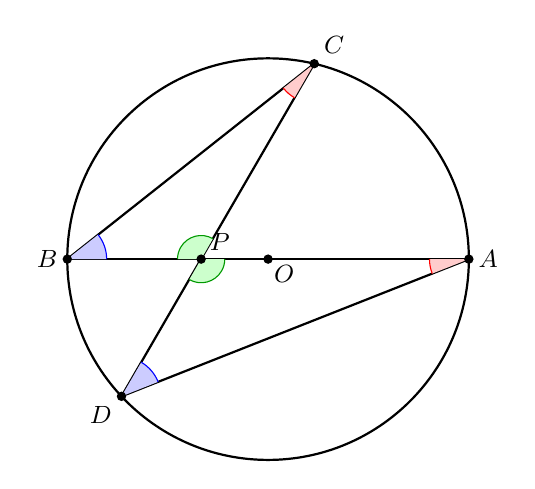
\begin{tikzpicture}[scale=0.85, font=\small\sffamily, line join=round]

    % O at origin, radius 3, P inside at (-1,0)
    % Chord AB through P and O: B=(-3,0), A=(3,0), order B-P-O-A
    % Chord CD through P at 60 degrees: C=(0.69,2.92), D=(-2.19,-2.05)
    \coordinate (O) at (0, 0);
    \coordinate (P) at (-1, 0);
    \coordinate (A) at (3, 0);
    \coordinate (B) at (-3, 0);
    \coordinate (C) at (0.69, 2.92);
    \coordinate (D) at (-2.19, -2.05);

    % Circle and all four triangle sides
    \draw[thick] (O) circle (3);
    \draw[thick] (B) -- (A);   % chord AB through O and P
    \draw[thick] (C) -- (D);   % chord CD through P
    \draw[thick] (B) -- (C);   % side of triangle PCB
    \draw[thick] (D) -- (A);   % side of triangle PAD

    % Red: angle PCB = angle PAD (inscribed angles subtending arc BD)
    \pic [draw=red, fill=red!20, angle radius=0.5cm] {angle = B--C--P};
    \pic [draw=red, fill=red!20, angle radius=0.5cm] {angle = P--A--D};

    % Blue: angle PBC = angle PDA (inscribed angles subtending arc CA)
    \pic [draw=blue, fill=blue!20, angle radius=0.5cm] {angle = P--B--C};
    \pic [draw=blue, fill=blue!20, angle radius=0.5cm] {angle = A--D--P};

    % Green: angle CPB = angle APD (vertical angles at P)
    \pic [draw=green!60!black, fill=green!20, angle radius=0.3cm] {angle = C--P--B};
    \pic [draw=green!60!black, fill=green!20, angle radius=0.3cm] {angle = D--P--A};

    % Segment labels
    %\node[above=2pt] at ($(P)!0.5!(A)$) {$PA$};
    %\node[above=2pt] at ($(P)!0.5!(B)$) {$PB$};
    %\node[above left=1pt] at ($(P)!0.5!(C)$) {$PC$};
    %\node[below left=1pt] at ($(P)!0.5!(D)$) {$PD$};

    % Points and labels
    \fill[black] (O) circle (2pt) node[below right, inner sep=2pt] {$O$};
    \fill[black] (P) circle (2pt) node[above right, inner sep=3pt] {$P$};
    \fill[black] (A) circle (2pt) node[right] {$A$};
    \fill[black] (B) circle (2pt) node[left] {$B$};
    \fill[black] (C) circle (2pt) node[above right] {$C$};
    \fill[black] (D) circle (2pt) node[below left] {$D$};

\end{tikzpicture}
\end{center}

Since $OA = OB = r$, we have $PO + OA = PA$ and $PO - OA = PO - OB = -PB$. Therefore,
\[
    \Pi(P) = PO^2 - OA^2 = (PO - OA)(PO + OA) = (-PB)(PA) = -PA \cdot PB.
\]
It suffices to show $PA \cdot PB = PC \cdot PD$, for then $\Pi(P) = -PC \cdot PD = -|\Pi(P)|$, giving $|\Pi(P)| = PC \cdot PD$.

Since $A$, $B$, $C$, $D$ all lie on the circle, the inscribed angles $\angle PCB$ and $\angle PAD$ both subtend arc $BD$ (\textcolor{red}{red}), so $\angle PCB = \angle PAD$; likewise $\angle PBC$ and $\angle PDA$ both subtend arc $CA$ (\textcolor{blue}{blue}). The angles $\angle CPB$ and $\angle APD$ are vertical angles at $P$ (\textcolor{green!60!black}{green}). By AA similarity,
\[
    \triangle PCB \sim \triangle PAD.
\]
Reading off corresponding sides:
\[
    \frac{PC}{PA} = \frac{PB}{PD} \implies PC \cdot PD = PA \cdot PB = |\Pi(P)|. \qedhere
\]
\end{proof}



\begin{remark}
    We now remark on the notion of signed length.
    In particular, we see that in the case where $P$ lies
    outside of the circle, we have that $\Pi(P)$ is positive, 
    and $\Pi(P) = PB * PC$. However, in the case where $P$ is 
    inside the circle, we have that $\Pi(P)$ is negative, and
    so $\Pi(P) = PB * PC$ doesn't entirely make sense if we are
    measuring $PB$ and $PC$ to both be positive lengths. However,
    to make sense of this since $P$ lies between the points $B$
    and $C$ on the line, if we choose an orientation of the line, 
    then one of these segments is positively orientated and the other
    is negatively orientated which explains why $\Pi(P)$ is negative
    for points inside the circle. 
\end{remark}

\section{Radical Axis}

We shall now discuss the radical axis, this relates the power of points between
two circles.

\begin{defn}
    The \textbf{radical axis} of two circles $O_1$ and $O_2$ (that may intersect)
    is the line $l$ such that for any $P\in l$, we have that $\Pi_1(P)=\Pi_2(P)$
    where $\Pi_i(P)$ is the power of the point $P$ with respect to the circle $O_i$. 
\end{defn}

We begin with some basic lemmas about the radical axis of two circles.

\begin{prop}
    Assume that circles $O_1$ and $O_2$ intersect at two points $A$ and $B$.
    Then the line $AB$ is the radical axis. 
\end{prop}

\begin{proof}
We show that every point $P$ on line $AB$ satisfies $\Pi_1(P) = \Pi_2(P)$, treating separately the cases where $P$ lies outside versus inside the two circles.

\begin{center}
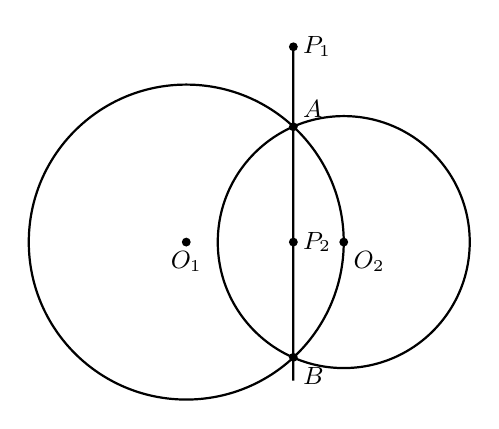
\begin{tikzpicture}[scale=0.8, font=\small\sffamily, line join=round]

    % O1=(-1,0) radius 2.5, O2=(1.5,0) radius 2
    % Radical axis at x=0.7; intersection points A=(0.7,1.83), B=(0.7,-1.83)
    % P1=(0.7,3.0) outside both circles, P2=(0.7,0) inside both circles
    \coordinate (O1) at (-1, 0);
    \coordinate (O2) at (1.5, 0);
    \coordinate (A)  at (0.7, 1.83);
    \coordinate (B)  at (0.7, -1.83);
    \coordinate (P1) at (0.7, 3.1);
    \coordinate (P2) at (0.7, 0);

    % Circles
    \draw[thick] (O1) circle (2.5);
    \draw[thick] (O2) circle (2);

    % Line AB extended through P1 above and slightly beyond B below
    \draw[thick] (P1) -- (0.7, -2.2);

    % Centers
    \fill[black] (O1) circle (2pt) node[below] {$O_1$};
    \fill[black] (O2) circle (2pt) node[below right] {$O_2$};

    % Points on the line
    \fill[black] (P1) circle (2pt) node[right] {$P_1$};
    \fill[black] (A)  circle (2pt) node[above right] {$A$};
    \fill[black] (P2) circle (2pt) node[right] {$P_2$};
    \fill[black] (B)  circle (2pt) node[below right] {$B$};

\end{tikzpicture}
\end{center}

\textbf{Case 1: $P_1$ on line $AB$, outside both circles.}
The line through $P_1$, $A$, $B$ is a secant to circle $O_1$ meeting it at $A$ and $B$. By the power of a point (tangent-secant theorem applied to the secant $P_1 A B$),
\[
    \Pi_1(P_1) = P_1A \cdot P_1B.
\]
The same line is also a secant to circle $O_2$ meeting it at the same points $A$ and $B$, so
\[
    \Pi_2(P_1) = P_1A \cdot P_1B.
\]
Hence $\Pi_1(P_1) = P_1A \cdot P_1B = \Pi_2(P_1)$.

\textbf{Case 2: $P_2$ on line $AB$, inside both circles.}
The segment $AB$ is a chord of circle $O_1$ passing through $P_2$. By the intersecting chords theorem,
\[
    \Pi_1(P_2) = -P_2A \cdot P_2B.
\]
The same chord lies inside circle $O_2$ as well, so
\[
    \Pi_2(P_2) = -P_2A \cdot P_2B.
\]
Hence $\Pi_1(P_2) = -P_2A \cdot P_2B = \Pi_2(P_2)$.

In both cases every point on line $AB$ has equal power with respect to the two circles, so $AB$ is the radical axis.
\end{proof}

We now state a theorem which describes the radical axes of three circles.

\begin{thm}
    Let $l_1,l_2,$ and $l_3$ be the radical axes of $O_2$ and $O_3$, $O_1$ and $O_3$, and $O_1$ and $O_2$ respectively.
    Then $l_1,l_2,$ and $l_3$ are concurrent.
\end{thm}

\begin{proof}
    Let $P$ be on the intersection of $l_1$ and $l_2$. We claim that $P$ is on $l_3$. Since $P\in l_1$, we have that $\Pi_2(P)=\Pi_3(P)$. 
    Now since $P\in l_2$, we have that $\Pi_1(P) = \Pi_3(P)$. Thus, we will have that $\Pi_1(P)=\Pi_2(P)=\Pi_3(P)$. Thus, $P\in l_2$. 

    In the case where each pair of circles intersects at two points, the three radical axes are precisely the lines through each pair of intersection points, and their concurrency at the radical center $R$ is illustrated below.

\begin{center}
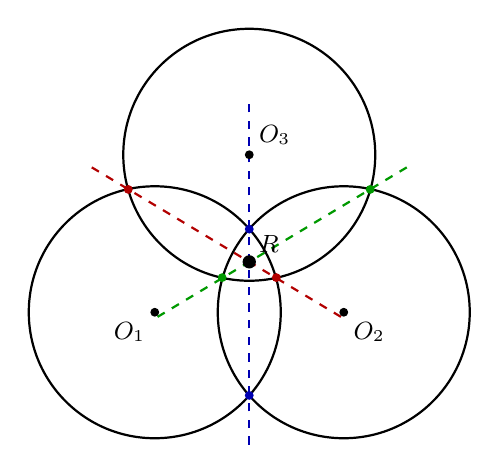
\begin{tikzpicture}[scale=0.8, font=\small\sffamily, line join=round]

    % O1=(0,0), O2=(3,0), O3=(1.5,2.5), all radius 2
    % Radical axes: O1-O2 at x=1.5 (blue), O1-O3 along 3x+5y=8.5 (red),
    %               O2-O3 along 3x-5y=0.5 (green). All meet at R=(1.5, 0.8).
    \coordinate (O1) at (0, 0);
    \coordinate (O2) at (3, 0);
    \coordinate (O3) at (1.5, 2.5);
    \coordinate (R)  at (1.5, 0.8);

    % Radical axes drawn first so circles appear in front
    \draw[dashed, blue!70!black, thick]  (1.5, -2.1) -- (1.5, 3.4);
    \draw[dashed, red!70!black,  thick]  (-1.0, 2.3) -- (3.0, -0.1);
    \draw[dashed, green!60!black, thick] (4.0, 2.3)  -- (0.0, -0.1);

    % Three circles
    \draw[thick] (O1) circle (2);
    \draw[thick] (O2) circle (2);
    \draw[thick] (O3) circle (2);

    % Pairwise intersection points, colored to match their radical axis
    \fill[blue!70!black]  (1.5,    1.32)  circle (2pt);
    \fill[blue!70!black]  (1.5,   -1.32)  circle (2pt);
    \fill[red!70!black]   (-0.42,  1.95)  circle (2pt);
    \fill[red!70!black]   (1.93,   0.55)  circle (2pt);
    \fill[green!60!black] (3.42,   1.95)  circle (2pt);
    \fill[green!60!black] (1.07,   0.55)  circle (2pt);

    % Radical center
    \fill[black] (R) circle (3pt) node[above right] {$R$};

    % Circle centers
    \fill[black] (O1) circle (2pt) node[below left]  {$O_1$};
    \fill[black] (O2) circle (2pt) node[below right] {$O_2$};
    \fill[black] (O3) circle (2pt) node[above right]       {$O_3$};

\end{tikzpicture}
\end{center}
\end{proof}

We remark that in the proof, we have assumed that the lines actually intersect. There is an edge case in which the radical 
axes are parallel. In this case, if we consider projective geometry, we can say that the lines are concurrent at infinity. 

Furthermore, using this theorem one can construct the radical axis of two non-intersecting circles. We leave this as an exercise. 


\section{Menalaus's Theorem}
We now will give a proof of Menalaus' theorem. 

\begin{thm}[Menalaus' Theorem]
    \verb|col A B F; col A C E; col B C D;|
    
    Then \verb|col D E F| $\Leftrightarrow\ \frac{AF}{BF}\cdot \frac{BD}{CD}\cdot\frac{CE}{AE} = 1$

    In particular, Menalus' theorem is saying that given a triangle $ABC$ where we extend the lines
    defining the triangle. Then if we draw a line which intersects each of the three lines defininig 
    the triangle at $DEF$, then we have a product of ratios is $1$ (and conversely given three points 
    on these lines that satisfy this ratio, then they lie on the same line). 
\end{thm}

Before proving Menalaus' Theorem, we remark that this theorem is another one in which it has a relationship
between a collinear and a ratio. Thus, such a theorem combines the angle table in AR with the ratio table in 
AR. However, in the next section when we discuss Ceva's theorem, we will see a caveat as to why implementing 
this theorem is quiet messy. 

\begin{proof}
We prove the forward direction: assuming $D$, $E$, $F$ are collinear, we show
$\dfrac{AF}{FB}\cdot\dfrac{BD}{CD}\cdot\dfrac{CE}{AE} = 1$.

\textbf{Construction.} Let $X$ be the point on line $AB$ such that $XC \parallel DEF$.

\begin{center}
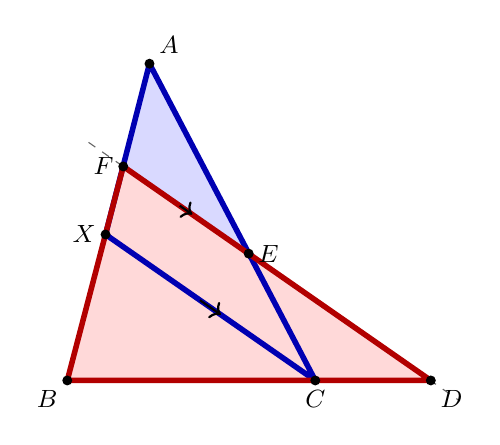
\begin{tikzpicture}[scale=0.9, font=\small\sffamily, line join=round]

    % Coordinates from Geogebra (D chosen to right of C; E on AC at t=0.6;
    % F = Intersect(AB, Line(D,E)); X = Intersect(AB, line through C parallel to DE))
    \coordinate (A) at (-3.47, 4.47);
    \coordinate (B) at (-4.63, 0);
    \coordinate (C) at (-1.13, 0);
    \coordinate (D) at (0.5, 0);
    \coordinate (E) at (-2.07, 1.79);
    \coordinate (F) at (-3.84, 3.02);
    \coordinate (X) at (-4.09, 2.06);

    % Shaded fills drawn first (behind everything else)
    \fill[blue!15] (A) -- (X) -- (C) -- cycle;
    \fill[red!15]  (B) -- (F) -- (D) -- cycle;

    % Main triangle and extended base (thin black, on top of fills)
    \draw[thick] (A) -- (B);
    \draw[thick] (B) -- (D);   % base B-C-D (D beyond C)
    \draw[thick] (C) -- (A);

    % Menelaus transversal line through D, E, F (dashed)
    \draw[dashed, gray!80!black] (-4.33, 3.36) -- (0.91, -0.29);

    % Triangle AXC: bold blue outline
    \draw[line width=2pt, blue!70!black] (A) -- (X) -- (C) -- cycle;

    % Triangle BFD: bold red outline
    \draw[line width=2pt, red!70!black] (B) -- (F) -- (D) -- cycle;

    % Parallel marks: same-direction arrows at midpoints of EF and XC
    \draw[->, thick] ($(F)!0.45!(E)$) -- ($(F)!0.55!(E)$);
    \draw[->, thick] ($(X)!0.45!(C)$) -- ($(X)!0.55!(C)$);

    % Points and labels
    \fill[black] (A) circle (2pt) node[above right] {$A$};
    \fill[black] (B) circle (2pt) node[below left]  {$B$};
    \fill[black] (C) circle (2pt) node[below]        {$C$};
    \fill[black] (D) circle (2pt) node[below right]  {$D$};
    \fill[black] (E) circle (2pt) node[right]         {$E$};
    \fill[black] (F) circle (2pt) node[left]          {$F$};
    \fill[black] (X) circle (2pt) node[left]          {$X$};

\end{tikzpicture}
\end{center}

\textbf{Step 1: $\triangle AXC \sim \triangle AFE$ (blue triangle).}
Since $XC \parallel FE$, we have $\angle AXC = \angle AFE$ (corresponding angles) and $\angle A$ is shared. By AA similarity, $\triangle AXC \sim \triangle AFE$, giving $AX/AF = AC/AE$. Since the order along line $AB$ is $A$--$F$--$X$--$B$, we have $AX = AF + FX$ and $AC = AE + EC$, so
\[
    \frac{AF + FX}{AF} = \frac{AE + EC}{AE} \implies \frac{FX}{AF} = \frac{EC}{AE}.
\]

\textbf{Step 2: $\triangle BXC \sim \triangle BFD$ (red triangle).}
Since $XC \parallel FD$, we have $\angle BXC = \angle BFD$ (corresponding angles) and $\angle B$ is shared. By AA similarity, $\triangle BXC \sim \triangle BFD$, giving $BX/BF = BC/BD$. Since $BX = BF - FX$ and $BC = BD - CD$,
\[
    \frac{BF - FX}{BF} = \frac{BD - CD}{BD} \implies \frac{FX}{BF} = \frac{CD}{BD} \implies \frac{BD}{CD} = \frac{BF}{FX}.
\]

\textbf{Conclusion.} Substituting into the product:
\[
    \frac{AF}{FB}\cdot\frac{BD}{CD}\cdot\frac{CE}{AE}
    = \frac{AF}{FB}\cdot\frac{BF}{FX}\cdot\frac{FX}{AF} = 1. 
\]

Now for the reverse direction. We shall assume that $\frac{AF}{FB}\cdot\frac{BD}{CD}\cdot\frac{CE}{AE}= 1.$
Now we shall take the points $D$ and $E$, and extend this line to intersect $AB$ at a point $F'$. Our goal is
to prove that $F = F'$. In particular, since \verb|col D E F'|, we have that 
\[
    \frac{AF'}{F'B}\cdot\frac{BD}{CD}\cdot\frac{CE}{AE} = 1. 
\]
Thus, we may conclude that 
\[
\frac{AF'}{F'B} = \frac{AF}{FB}.
\]
Now we shall add $1=\frac{F'B}{F'B}=\frac{FB}{FB}$ to both sides and use the fact that 
$AF'+F'B = AB$ and $AF + FB = AB$ to conclude that 
\[
\frac{AF'+F'B}{F'B}=\frac{AF+FB}{FB}\Rightarrow\frac{AB}{F'B}=\frac{AB}{FB}\Rightarrow F'B = FB.
\]
Thus, as the distance from $F$ to $B$ and $F'$ to $B$ are the same and we have that both $F$ and $F'$
lie on the line $AB$, we may conclude that $F=F'$.
\end{proof}

We remark that there are really two choices of $F'$ that are the same distance from $B$ as $F$ on the line
$AB$; however, if one considers the signed distance this forces $F'=F$ in the above proof. 

\section{Ceva's Theorem}

We now will give a proof of Ceva's theorem. 

\begin{thm}[Ceva's Theorem]
    \verb|col A B F; col A C E; col B C D;|

    Then \verb|concurrent A D B E C F| $\Leftrightarrow\ \frac{AF}{BF}\cdot \frac{BD}{CD}\cdot\frac{CE}{AE} = 1$
\end{thm}

\begin{remark}
    We now discuss the reason Menalaus' and Ceva's theorems are difficult to implement. In particular,
    the statements of the two theorems are nearly identical. The only difference is that we have either:
    \verb|col D E F| or \verb|concurrent A D B E C F|. The difference between the two comes down to the 
    notion of the signed distance. Since in the case of Menalaus' theorem, we will have that ratio of the 
    signed distances will actually be $-1$ as two of the points lie inbetween the segments of the triangle. 
\end{remark}

\begin{proof}

We begin with the forward direction. Suppose the lines $AD$, $BE$, and $CF$ are concurrent at an interior point $X$.
We will show $\dfrac{AF}{FB}\cdot\dfrac{BD}{CD}\cdot\dfrac{CE}{AE} = 1$.
Denote the area of $\triangle XYZ$ by $[XYZ]$.

\begin{center}
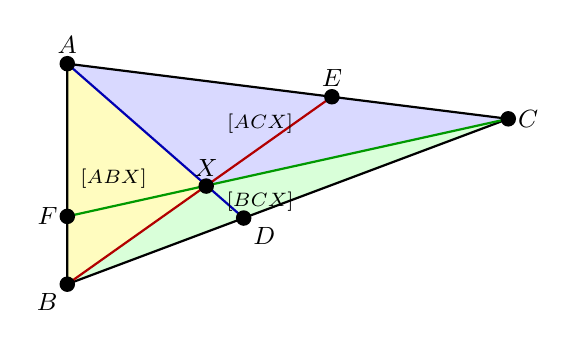
\begin{tikzpicture}[scale=1.4, font=\small\sffamily, line join=round]
    \coordinate (A) at (-2, 2);
    \coordinate (B) at (-2, 0);
    \coordinate (C) at (2, 1.5);
    \coordinate (D) at (-0.4, 0.6);
    \coordinate (E) at (0.4, 1.7);
    \coordinate (F) at (-2, 0.615);
    \coordinate (X) at (-0.74, 0.89);

    % Shade the three inner triangles (fills first, behind everything)
    \fill[yellow!25] (A) -- (B) -- (X) -- cycle;
    \fill[green!15]  (B) -- (C) -- (X) -- cycle;
    \fill[blue!15]   (A) -- (C) -- (X) -- cycle;

    % Main triangle
    \draw[thick] (A) -- (B) -- (C) -- cycle;

    % Three concurrent cevians in distinct colors
    \draw[thick, blue!70!black]  (A) -- (D);
    \draw[thick, red!70!black]   (B) -- (E);
    \draw[thick, green!60!black] (C) -- (F);

    % Area labels at centroids of each inner triangle
    \node[font=\scriptsize] at (-1.58, 0.96) {$[ABX]$};
    \node[font=\scriptsize] at (-0.25, 0.75) {$[BCX]$};
    \node[font=\scriptsize] at (-0.25, 1.46) {$[ACX]$};

    % Point labels
    \fill[black] (A) circle (2pt) node[above]      {$A$};
    \fill[black] (B) circle (2pt) node[below left]  {$B$};
    \fill[black] (C) circle (2pt) node[right]        {$C$};
    \fill[black] (D) circle (2pt) node[below right]  {$D$};
    \fill[black] (E) circle (2pt) node[above]        {$E$};
    \fill[black] (F) circle (2pt) node[left]         {$F$};
    \fill[black] (X) circle (2pt) node[above]        {$X$};
\end{tikzpicture}
\end{center}

\textbf{Claim 1:} $\dfrac{BD}{CD} = \dfrac{[ABX]}{[ACX]}$.

Triangles $\triangle ABD$ and $\triangle ACD$ share the altitude from $A$ to line $BC$, so
\[
    \frac{[ABD]}{[ACD]} = \frac{BD}{CD}.
\]
Triangles $\triangle XBD$ and $\triangle XCD$ share the altitude from $X$ to line $BC$, so
\[
    \frac{[XBD]}{[XCD]} = \frac{BD}{CD}.
\]
Since $X$ lies on segment $\overline{AD}$, we have $[ABD] = [ABX] + [XBD]$ and $[ACD] = [ACX] + [XCD]$. Subtracting:
\[
    \frac{BD}{CD} = \frac{[ABD] - [XBD]}{[ACD] - [XCD]} = \frac{[ABX]}{[ACX]}.
\]

\textbf{Claim 2:} $\dfrac{CE}{AE} = \dfrac{[BCX]}{[ABX]}$.

Applying the same argument to the line $\overline{BE}$, with $X$ on segment $\overline{BE}$ and $E$ on $\overline{CA}$: triangles $\triangle BCE$ and $\triangle ABE$ share the altitude from $B$ to $CA$, while $\triangle XCE$ and $\triangle XAE$ share the altitude from $X$ to $CA$. Since $[BCE] = [BCX] + [XCE]$ and $[ABE] = [ABX] + [XAE]$:
\[
    \frac{CE}{AE} = \frac{[BCE] - [XCE]}{[ABE] - [XAE]} = \frac{[BCX]}{[ABX]}.
\]

\textbf{Claim 3:} $\dfrac{AF}{FB} = \dfrac{[ACX]}{[BCX]}$.

Applying the same argument to the line $\overline{CF}$, with $X$ on segment $\overline{CF}$ and $F$ on $\overline{AB}$: triangles $\triangle ACF$ and $\triangle BCF$ share the altitude from $C$ to $AB$, while $\triangle XAF$ and $\triangle XBF$ share the altitude from $X$ to $AB$. Since $[ACF] = [ACX] + [XAF]$ and $[BCF] = [BCX] + [XBF]$:
\[
    \frac{AF}{FB} = \frac{[ACF] - [XAF]}{[BCF] - [XBF]} = \frac{[ACX]}{[BCX]}.
\]

Multiplying the three claims, the areas telescope:
\[
    \frac{AF}{FB}\cdot\frac{BD}{CD}\cdot\frac{CE}{AE}
    \;=\; \frac{[ACX]}{[BCX]}\cdot\frac{[ABX]}{[ACX]}\cdot\frac{[BCX]}{[ABX]} \;=\; 1.\qedhere
\]

The proof above covers the case where $D$, $E$, $F$ all lie on the sides of $\triangle ABC$, so the concurrency point $X$ lies \emph{inside} the triangle. The same argument applies when some of these points lie on extensions of the sides, in which case $X$ lies \emph{outside} the triangle.

\begin{center}
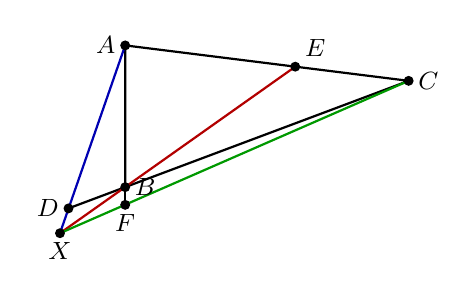
\begin{tikzpicture}[scale=0.9, font=\small\sffamily, line join=round]
    \coordinate (A) at (-2, 2);
    \coordinate (B) at (-2, 0);
    \coordinate (C) at (2, 1.5);
    \coordinate (D) at (-2.8, -0.3);    % line BC extended, left of B
    \coordinate (E) at (0.4, 1.7);      % segment CA (between C and A)
    \coordinate (F) at (-2, -0.25);     % line AB extended, below B
    \coordinate (X) at (-2.92, -0.65);  % concurrency point, outside ABC

    % Triangle ABC
    \draw[thick] (A) -- (B) -- (C) -- cycle;

    % Dashed extensions of BC past B to D, and of AB past B to F
    \draw[thick] (B) -- (D);
    \draw[thick] (B) -- (F);

    % Three cevian lines, all meeting at X outside the triangle
    \draw[thick, blue!70!black]  (A) -- (X);   % through D on BC extended
    \draw[thick, red!70!black]   (E) -- (X);   % through B
    \draw[thick, green!60!black] (C) -- (X);   % through F on AB extended

    % Points
    \fill[black] (A) circle (2pt) node[left]        {$A$};
    \fill[black] (B) circle (2pt) node[right]        {$B$};
    \fill[black] (C) circle (2pt) node[right]        {$C$};
    \fill[black] (D) circle (2pt) node[left]   {$D$};
    \fill[black] (E) circle (2pt) node[above right]  {$E$};
    \fill[black] (F) circle (2pt) node[below]         {$F$};
    \fill[black] (X) circle (2pt) node[below]        {$X$};
\end{tikzpicture}
\end{center}

Here $D$ lies on the extension of $\overline{BC}$ beyond $B$, $F$ lies on the extension of $\overline{AB}$ beyond $B$, and $X$ lies outside $\triangle ABC$. In this configuration $X$ lies beyond $D$ on line $AD$ (order: $A$--$D$--$X$), so the area decomposition in each claim \emph{adds} instead of subtracts. For Claim~1, since $[ABX] = [ABD]+[XBD]$ and $[ACX]=[ACD]+[XCD]$:
\[
    \frac{BD}{CD} = r
    \;\Longrightarrow\;
    \frac{[ABX]}{[ACX]} = \frac{[ABD]+[XBD]}{[ACD]+[XCD]}
    = \frac{r\,[ACD]+r\,[XCD]}{[ACD]+[XCD]} = r,
\]
and analogous additions hold in Claims~2 and~3. The telescoping product is identical, so $\frac{AF}{FB}\cdot\frac{BD}{CD}\cdot\frac{CE}{AE}=1$ in both cases.

Now for the converse. The proof is analogous to the converse of Menalaus' theorem. In particular, if we have that $BE$ and $CF$ intersect at the point $X$.
Then if we draw the line from $AX$ and say it intersects at the point $D'$ on the line $BC$. The claim will be that $D=D'$. From the forward direction of 
Ceva's theorem since the lines are concurrent, we have that 
\[
\dfrac{AF}{FB}\cdot\dfrac{BD'}{CD'}\cdot \dfrac{CE}{AE} = 1.
\]
Now in a similar way to the converse of Menalaus' theorem, we will havve that 
\[
\dfrac{BD }{DC} = \dfrac{BD'}{D'C}.
\]
Thus, in a similar way to the proof of Menalaus' theorem, we will have that $D=D'$. 
\end{proof}


\section{Pappus's Theorem}

We now prove Pappus's Hexagon Theorem. 

\begin{thm}[Pappus's Hexagon Theorem]
    Given \verb|col A E C; col D B F|, then draw the ``hexagon'' \verb|ABCDEF|, and let 
    $X$, $Y$, and $Z$ be the intersections of the opposite sides of the hexagon, then \verb|col X Y Z|.
\end{thm}

\begin{proof}
    We consider the configuration where the line $DE$ is not parallel to the line $BC$. 
Let $P$ be the intersection of $DE$ with $BC$. 
Let $Q$ be the intersection of $DE$ with $AF$. 
Let $R$ be the intersection of $BC$ with $AF$. 

We see this in the figure below:

\begin{figure}[h]
    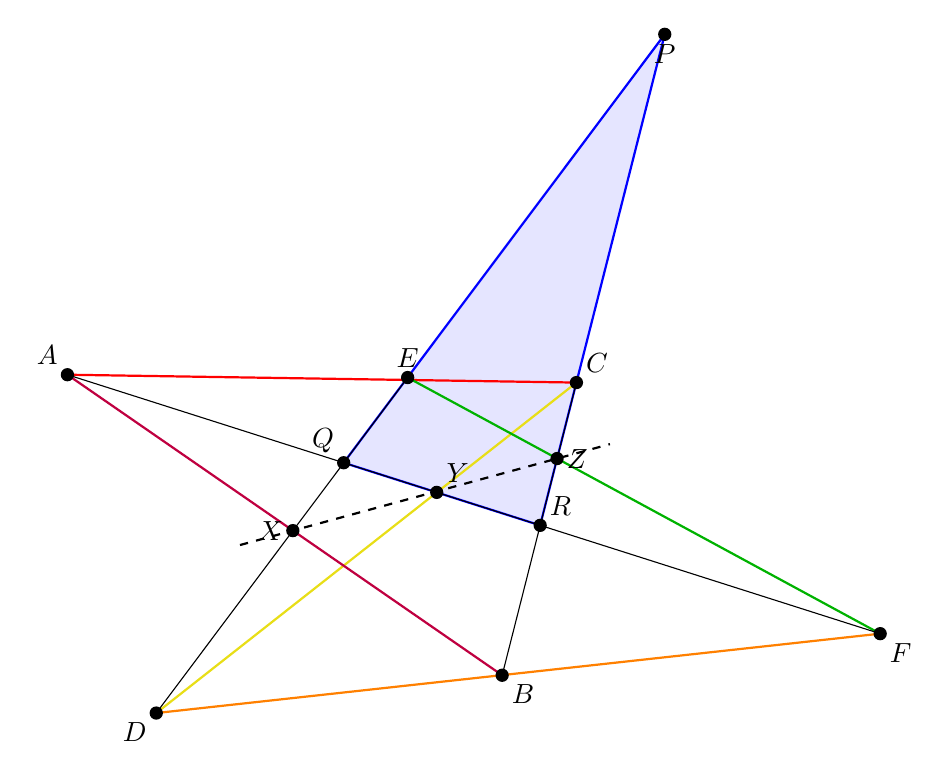
\begin{tikzpicture}[scale=1.2]

        % 1. Define the base coordinate points
        \coordinate (A) at (-6.5, 1.61);
        \coordinate (C) at (-1.11415, 1.52688);
        \coordinate (E) at (-2.9, 1.58); % On line AC
        
        \coordinate (D) at (-5.56, -1.97);
        \coordinate (B) at (-1.9, -1.57);
        \coordinate (F) at (2.1, -1.13); % On line BD
    
        % 2. Calculate the intersection points for Triangle PQR
        % P = BC \cap DE
        \coordinate (P) at (intersection of B--C and D--E);
        % Q = DE \cap FA
        \coordinate (Q) at (intersection of D--E and F--A);
        % R = BC \cap FA
        \coordinate (R) at (intersection of B--C and F--A);
    
        % 3. Draw and color Triangle PQR
        \fill[blue!10] (P) -- (Q) -- (R) -- cycle;
        \draw[blue, thick] (P) -- (Q) -- (R) -- cycle;
    
        % 4. Calculate the remaining Pappus intersection points (X, Y, Z)
        % X = AB \cap DE
        \coordinate (X) at (intersection of A--B and D--E);
        % Y = CD \cap FA
        \coordinate (Y) at (intersection of C--D and F--A);
        % Z = BC \cap EF
        \coordinate (Z) at (intersection of B--C and E--F);
    
        % 5. Draw the 5 Menelaus line segments with requested colors
        \draw[red, thick] (A) -- (C);                  % Line AEC
        \draw[orange, thick] (D) -- (F);               % Line DBF
        \draw[yellow!90!black, thick] (D) -- (C);      % Line DYC (darkened slightly for visibility)
        \draw[green!70!black, thick] (E) -- (F);       % Line EZF
        \draw[purple, thick] (A) -- (B);               % Line AXB
        
        % Draw the remaining connecting segments for completeness
        \draw (B) -- (C); % Line BC
        \draw (A) -- (F); % Line AF
        \draw (D) -- (E); % Line DE
    
        % 6. Draw the Pappus Line connecting X, Y, and Z
        \draw[black, thick, dashed] ($ (X) ! -0.2 ! (Z) $) -- ($ (X) ! 1.2 ! (Z) $);
    
        % 7. Draw and label all points
        \foreach \pt/\pos in {
            A/above left, C/above right, E/above, 
            D/below left, B/below right, F/below right, 
            P/below, Q/above left, R/above right,
            X/left, Y/above right, Z/right%
        } {
            \fill (\pt) circle (2pt) node[\pos] {$\pt$};
        }
    
    \end{tikzpicture}
\end{figure}

We apply Menelaus's Theorem to the central triangle $\triangle PQR$ (highlighted blue) using the five specified transversal lines ($AEC$, $DBF$, $DYC$, $EZF$, and $AXB$). Because these lines intersect the extended sides of $\triangle PQR$, the product of the directed ratios of the segments equals $-1$.

\begin{enumerate}
    \item Line $AEC$ (red line) intersecting $\triangle PQR$:
    \[ \frac{PE}{EQ} \cdot \frac{QA}{AR} \cdot \frac{RC}{CP} = -1 \]
    
    \item Line $DBF$ (orange line) intersecting $\triangle PQR$:
    \[ \frac{PD}{DQ} \cdot \frac{QF}{FR} \cdot \frac{RB}{BP} = -1 \]
    
    \item Line $DYC$ (yellow line) intersecting $\triangle PQR$:
    \[ \frac{PD}{DQ} \cdot \frac{QY}{YR} \cdot \frac{RC}{CP} = -1 \]
    
    \item Line $EZF$ (green line) intersecting $\triangle PQR$:
    \[ \frac{PE}{EQ} \cdot \frac{QF}{FR} \cdot \frac{RZ}{ZP} = -1 \]
    
    \item Line $AXB$ (purple line) intersecting $\triangle PQR$:
    \[ \frac{PX}{XQ} \cdot \frac{QA}{AR} \cdot \frac{RB}{BP} = -1 \]
\end{enumerate}

We observe that equations 3, 4, and 5 contain the specific segment ratios $\frac{QY}{YR}$, $\frac{RZ}{ZP}$, and $\frac{PX}{XQ}$ needed to establish the collinearity of $X$, $Y$, and $Z$ (dotted line) with respect to $\triangle PQR$. 

To isolate these terms, we multiply equations 3, 4, and 5 together, and then multiply by the inverses of equations 1 and 2:

\[
\left( \frac{PD}{DQ} \cdot \frac{QY}{YR}\cdot  \frac{RC}{CP} \right) \left( \frac{PE}{EQ}\cdot \frac{QF}{FR} \cdot \frac{RZ}{ZP} \right) \left( \frac{PX}{XQ} \cdot \frac{QA}{AR}\cdot  \frac{RB}{BP} \right) \left( \frac{EQ}{PE}\cdot \frac{AR}{QA}\cdot \frac{CP}{RC} \right) \left( \frac{DQ}{PD}\cdot \frac{FR}{QF} \cdot\frac{BP}{RB} \right) = -1
\]

Regrouping the fractions to cancel corresponding terms:

\[
\left( \frac{PD}{DQ}\cdot \frac{DQ}{PD} \right) \left( \frac{RC}{CP}\cdot \frac{CP}{RC} \right) \left( \frac{PE}{EQ}\cdot \frac{EQ}{PE} \right) \left( \frac{QF}{FR}\cdot \frac{FR}{QF} \right) \left( \frac{QA}{AR}\cdot \frac{AR}{QA} \right) \left( \frac{RB}{BP}\cdot \frac{BP}{RB} \right) \left( \frac{PX}{XQ} \cdot \frac{QY}{YR} \cdot \frac{RZ}{ZP} \right) = -1
\]

All of the intermediate ratios cancel perfectly to $1$, leaving only:

\[
\frac{PX}{XQ} \cdot \frac{QY}{YR} \cdot \frac{RZ}{ZP} = -1
\]

By the converse of Menelaus's Theorem, because the product of the directed ratios along the sides of $\triangle PQR$ equals $-1$, the points $X$, $Y$, and $Z$ must be collinear.
\end{proof}

\begin{remark}
    We remark that the proof we have provided uses the point $P$ which is the intersectoin of $DE$ and $BC$, and when $AB$ is parallel to $EF$; however, if these
    pairs of lines are parallel, then the proof which we have provided does not work. We leave this case as an exercise to the reader. 
\end{remark}

\section{Pascal's Theorem}

We now prove Pascal's Hexagon Theorem.

\begin{thm}[Pascal's Hexagon Theorem]
Assume that a hexagon $ABCDEF$ is inscribed in a circle and let $X$, $Y$, $Z$ be the intersections of opposite sides, then \verb|col X Y Z|.
\end{thm}

\begin{proof}
    Given the hexagon $ABCDEF$ inscribed in a circle, we let $G$ be the intersection of lines $AF$ and $BC$, $H$ be the intersection of lines $AF$ and $DE$, and $I$ be the intersection of lines $BC$ and $DE$. This forms the (blue) triangle $\triangle GHI$.
    We observe this in the diagram below:
    \begin{figure}[h]
        \begin{center}
            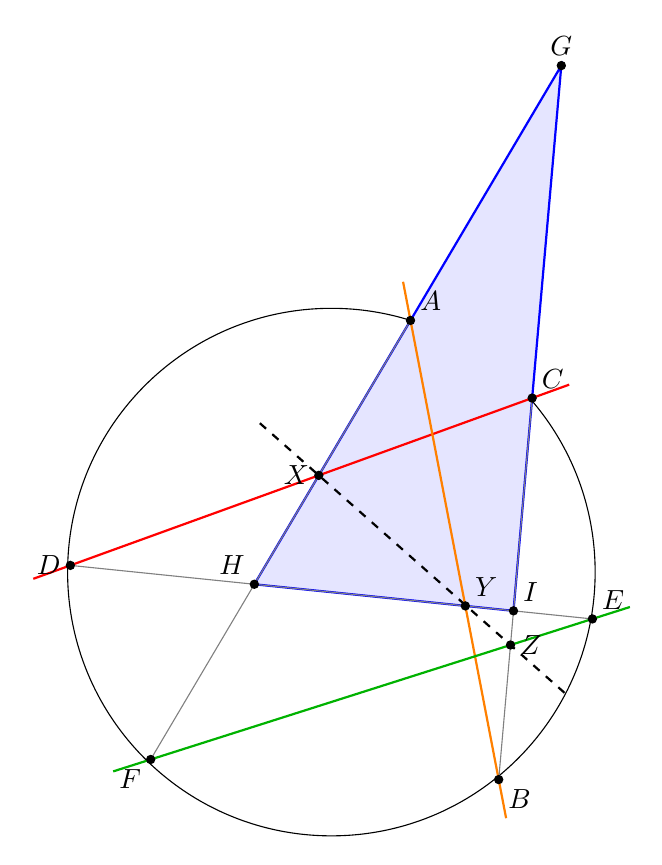
\begin{tikzpicture}[scale=0.85]
            
                % 1. Define the center and draw the circumscribed circle
                \coordinate (O) at (0,0);
                \draw (O) circle (3.941);
            
                % 2. Define the coordinates for the hexagon A,B,C,D,E,F
                \coordinate (A) at (1.18225, 3.75995);
                \coordinate (B) at (2.5, -3.1);
                \coordinate (C) at (3, 2.6);
                \coordinate (D) at (-3.9, 0.1);
                \coordinate (E) at (3.9, -0.7);
                \coordinate (F) at (-2.7, -2.8);
            
                % 3. Calculate intersections for Triangle GHI
                % G = BC \cap FA
                \coordinate (G) at (intersection of B--C and F--A);
                % H = ED \cap FA
                \coordinate (H) at (intersection of E--D and F--A);
                % I = ED \cap BC
                \coordinate (I) at (intersection of E--D and B--C);
            
                % 4. Draw and highlight Triangle GHI
                \fill[blue!10] (G) -- (H) -- (I) -- cycle;
                \draw[blue, thick] (G) -- (H) -- (I) -- cycle;
            
                % 5. Calculate the Pascal line points X, Y, Z
                % X = CD \cap FA
                \coordinate (X) at (intersection of C--D and F--A);
                % Y = AB \cap ED
                \coordinate (Y) at (intersection of A--B and E--D);
                % Z = EF \cap BC
                \coordinate (Z) at (intersection of E--F and B--C);
            
                % 6. Draw the Menelaus transversals with requested colors
                % We extend the lines slightly past the points for visual clarity
                \draw[red, thick, shorten <=-0.5cm, shorten >=-0.5cm] (C) -- (D) node[midway, sloped, above] {}; % Line DXC (CD extended)
                \draw[orange, thick, shorten <=-0.5cm, shorten >=-0.5cm] (A) -- (B); % Line AYB (AB extended)
                \draw[green!70!black, thick, shorten <=-0.5cm, shorten >=-0.5cm] (E) -- (F); % Line EZF (EF extended)
            
                % Draw remaining hexagon segments
                \draw[gray, thin] (B) -- (C);
                \draw[gray, thin] (D) -- (E);
                \draw[gray, thin] (F) -- (A);
            
                % 7. Draw the Pascal Line connecting X, Y, and Z
                \draw[black, thick, dashed, shorten <=-1cm, shorten >=-1cm] (X) -- (Z);
            
                % 8. Label all points
                \foreach \pt/\pos in {
                    A/above right, B/below right, C/above right, 
                    D/left, E/above right, F/below left,
                    G/above, H/above left, I/above right,
                    X/left, Y/above right, Z/right%
                } {
                    \fill (\pt) circle (2pt) node[\pos] {$\pt$};
                }
            
            \end{tikzpicture}
            \end{center}        
    \end{figure}

We now apply Menelaus's Theorem to the transversal lines $DXC$ (red line), $AYB$ (orange line), and $EZF$ (green line) with respect to the (blue) triangle $\triangle GHI$. Because these transversals intersect the extended sides of the triangle, the product of their directed ratios is $-1$:

\begin{enumerate}
    \item (Red) Line $DXC$ intersecting $\triangle GHI$:
    \[ \frac{GC}{CI} \cdot \frac{ID}{DH} \cdot \frac{HX}{XG} = -1 \]
    
    \item (Orange) Line $AYB$ intersecting $\triangle GHI$:
    \[ \frac{HA}{AG} \cdot \frac{GB}{BI} \cdot \frac{IY}{YH} = -1 \]
    
    \item (Green) Line $EZF$ intersecting $\triangle GHI$:
    \[ \frac{HF}{FG} \cdot \frac{GZ}{ZI} \cdot \frac{IE}{EH} = -1 \]
\end{enumerate}

We can see that the ratios $\frac{HX}{XG}$, $\frac{IY}{YH}$, and $\frac{GZ}{ZI}$ are the exact three components we need to apply the converse of Menelaus's theorem for the line $XYZ$ with respect to $\triangle GHI$. 

To isolate these terms, we multiply all three equations together. Grouping the intersections $G$, $H$, and $I$ with their corresponding intersecting chords on the circle yields the following equations by the Power of a Point (Intersecting Chords) Theorem:

\begin{align*}
    \frac{DI \cdot IE}{BI \cdot IC} &= 1 \\
    \frac{BG \cdot GC}{AG \cdot GF} &= 1 \\
    \frac{AH \cdot HF}{DH \cdot HE} &= 1
\end{align*}

Thus, when we multiply the three Menelaus equations together and apply these power of a point identities, the lengths of the circle's chords cancel out perfectly to $1$:

\[
\left( \frac{GC \cdot GB}{AG \cdot FG} \right) \left( \frac{HA \cdot HF}{DH \cdot EH} \right) \left( \frac{ID \cdot IE}{CI \cdot BI} \right) \left( \frac{HX}{XG} \cdot \frac{IY}{YH} \cdot \frac{GZ}{ZI} \right) = -1
\]

\[
(1) \cdot (1) \cdot (1) \cdot \left( \frac{HX}{XG} \cdot \frac{IY}{YH} \cdot \frac{GZ}{ZI} \right) = -1
\]

This simplifies to:
\[
\frac{HX}{XG} \cdot \frac{IY}{YH} \cdot \frac{GZ}{ZI} = -1
\]

By the converse to Menelaus's theorem, because the product of the directed ratios along the sides of $\triangle GHI$ equals $-1$, we conclude that the points $X$, $Y$, and $Z$ must be collinear.
\end{proof}

\begin{remark}
    Similar to Pappus's theorem, our proof relied on a simplification where we had the intersection points of $G$, $H$, and $I$.
    If the corresponding lines are parallel, then the intersections are points at inifinity, and the theorem is still true, but an
    additional proof is necessary. 
\end{remark}

\section{Brianchon's Theorem}

We will now discuss Brianchon's theorem. 

\begin{thm}
    Assume that a circle is inscribed in a hexagon $ABCDEF$, then $AD$, $BE$, and $CF$ are concurrent. 
\end{thm}

\begin{figure}[h]
    \begin{center}
        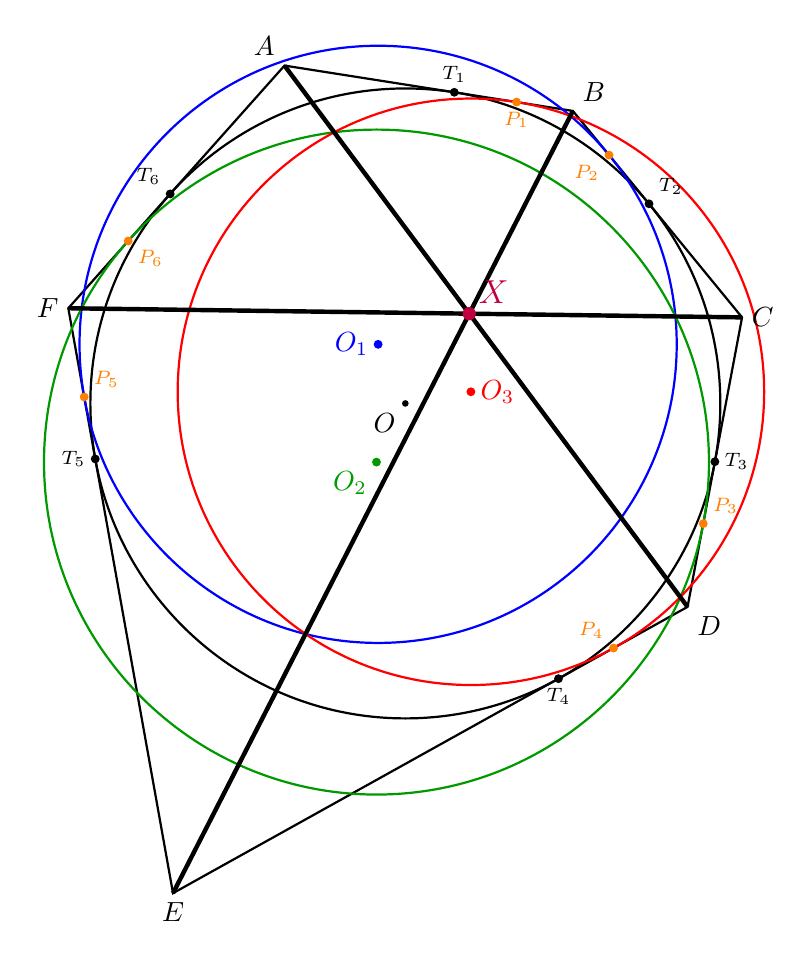
\begin{tikzpicture}[scale=0.8]
        
            % 1. The Incircle
            \draw[black, thick] (0,0) circle (5);
            \fill (0,0) circle (1.5pt) node[below left] {$O$};
            
            % 2. Vertices of the Hexagon
            \coordinate (A) at (-1.918, 5.363);
            \coordinate (B) at (2.660, 4.643);
            \coordinate (C) at (5.345, 1.366);
            \coordinate (D) at (4.480, -3.229);
            \coordinate (E) at (-3.688, -7.774);
            \coordinate (F) at (-5.350, 1.511);
        
            % Draw the circumscribed hexagon (Tangents)
            \draw[thick, black] (A) -- (B) -- (C) -- (D) -- (E) -- (F) -- cycle;
        
            % 3. Tangency Points
            \coordinate (T1) at (0.777, 4.939);
            \coordinate (T2) at (3.868, 3.169);
            \coordinate (T3) at (4.914, -0.925);
            \coordinate (T4) at (2.431, -4.369);
            \coordinate (T5) at (-4.922, -0.881);
            \coordinate (T6) at (-3.733, 3.326);
        
            % 4. Shifted Offset Points
            \coordinate (P1) at (1.765, 4.784);
            \coordinate (P2) at (3.234, 3.942);
            \coordinate (P3) at (4.729, -1.908);
            \coordinate (P4) at (3.305, -3.883);
            \coordinate (P5) at (-5.098, 0.103);
            \coordinate (P6) at (-4.399, 2.579);
        
            % 5. Auxiliary Circle Centers
            \coordinate (O1) at (-0.432, 0.938);
            \coordinate (O2) at (-0.458, -0.931);
            \coordinate (O3) at (1.041, 0.185);
        
            % Draw Auxiliary Circles C1, C2, C3
            % Radii calculated from distances: O_i to P_i
            \draw[thick, blue] (O1) circle (4.740);
            \draw[thick, green!60!black] (O2) circle (5.278);
            \draw[thick, red] (O3) circle (4.655);
        
            % 6. The Principal Diagonals (Radical Axes)
            \draw[ultra thick, black] (A) -- (D);
            \draw[ultra thick, black] (B) -- (E);
            \draw[ultra thick, black] (C) -- (F);
        
            % 7. The Brianchon Center (Renamed to X)
            \coordinate (X) at (1.014, 1.425);
            \fill[purple] (X) circle (3pt) node[above right, font=\large] {$X$};
        
            % 8. Plot Tangency Points
            \foreach \pt/\pos/\name in {
                T1/above/T_1, T2/above right/T_2, T3/right/T_3,
                T4/below/T_4, T5/left/T_5, T6/above left/T_6
            } {
                \fill[black] (\pt) circle (2pt) node[\pos, font=\scriptsize, text=black] {$\name$};
            }
        
            % 9. Plot Shifted Offset Points
            \foreach \pt/\pos/\name in {
                P1/below/P_1, P2/below left/P_2, P3/above right/P_3,
                P4/above left/P_4, P5/above right/P_5, P6/below right/P_6
            } {
                \fill[orange] (\pt) circle (2pt) node[\pos, font=\scriptsize] {$\name$};
            }
        
            % 10. Label Hexagon Vertices
            \node[above left] at (A) {$A$};
            \node[above right] at (B) {$B$};
            \node[right] at (C) {$C$};
            \node[below right] at (D) {$D$};
            \node[below] at (E) {$E$};
            \node[left] at (F) {$F$};
            
            % 11. Label Circle Centers
            \fill[blue] (O1) circle (2pt) node[left] {$O_1$};
            \fill[green!60!black] (O2) circle (2pt) node[below left] {$O_2$};
            \fill[red] (O3) circle (2pt) node[right] {$O_3$};
        
        \end{tikzpicture}
        \end{center}
\end{figure}

\begin{proof}


    Let the hexagon $ABCDEF$ be circumscribed around a circle $\omega$ with center $O$ (black circle). Let the points of tangency of $\omega$ with the sides $AB$, $BC$, $CD$, $DE$, $EF$, and $FA$ be $T_1$, $T_2$, $T_3$, $T_4$, $T_5$, and $T_6$ respectively.

Because the sides of the hexagon are tangent to the inscribed circle, the tangent segments drawn from each vertex to the incircle are equal in length. We denote these lengths as:
\begin{align*}
    a &= AT_1 = AT_6 \\
    b &= BT_1 = BT_2 \\
    c &= CT_2 = CT_3 \\
    d &= DT_3 = DT_4 \\
    e &= ET_4 = ET_5 \\
    f &= FT_5 = FT_6
\end{align*}

To construct our three specific circles, we shift the points of tangency by a small, arbitrary distance $k > 0$ along the perimeter of the hexagon. We plot six new points, $P_1$ through $P_6$ (labeled in orange), on the sides by alternately adding and subtracting $k$:
\begin{itemize}
    \item On side $AB$, plot $P_1$ such that $AP_1 = a + k$ and $BP_1 = b - k$.
    \item On side $BC$, plot $P_2$ such that $BP_2 = b - k$ and $CP_2 = c + k$.
    \item On side $CD$, plot $P_3$ such that $CP_3 = c + k$ and $DP_3 = d - k$.
    \item On side $DE$, plot $P_4$ such that $DP_4 = d - k$ and $EP_4 = e + k$.
    \item On side $EF$, plot $P_5$ such that $EP_5 = e + k$ and $FP_5 = f - k$.
    \item On side $FA$, plot $P_6$ such that $FP_6 = f - k$ and $AP_6 = a + k$.
\end{itemize}

By alternating the arithmetic sign of the shift $k$, the distances from each vertex to its two adjacent offset points remain perfectly equal: 
\[ AP_1 = AP_6, \quad BP_1 = BP_2, \quad CP_2 = CP_3, \quad DP_3 = DP_4, \quad EP_4 = EP_5, \quad FP_5 = FP_6 \]

We now define three auxiliary circles $C_1$ (blue), $C_2$ (green), and $C_3$ (red) that are tangent to opposite sides of the hexagon at these new shifted points:
\begin{itemize}
    \item Let $C_1$ be the (blue) circle tangent to $BC$ at $P_2$ and tangent to $EF$ at $P_5$.
    \item Let $C_2$ be the (green) circle tangent to $CD$ at $P_3$ and tangent to $FA$ at $P_6$.
    \item Let $C_3$ be the (red) circle tangent to $AB$ at $P_1$ and tangent to $DE$ at $P_4$.
\end{itemize}

We remark that the reason that these circles exists is due to the uniform shift of the $T_i$. Since we have that given two lines and two points on those lines, then a 
circle exists which is tangent to both of these lines at the two specified points exists if and only if the distance from the point of intersection to the two specified points is the same. 
For example, we see that the circle $C_1$ exists as follows. We want $C_1$ to be tangent to $BC$ and $EF$. Then if we let $R$ be the point of intersection of $BC$ and $EF$. Then since the circle
$\omega$ is tangent to $BC$ and $EF$ at $T_2$ and $T_5$. We know that the $\overline{RT_2}=\overline{RT_5}$. Then we will have that $\overline{RP_2}=\overline{RP_5}$ since we will just be adjusting
the distance by a factor of $k$ from the intersection point. 

We now find the radical axes for these three pairs of circles. The power of a point outside a circle is the square of the distance from the point to the circle's point of tangency.

\begin{enumerate}
    \item \textbf{Circles $C_2$ and $C_3$:} 
    The power of vertex $A$ to $C_3$ (red) is $AP_1^2$, and its power to $C_2$ (green) is $AP_6^2$. Since $AP_1 = AP_6$, vertex $A$ has equal power to both circles. Similarly, the power of vertex $D$ to $C_3$ (red) is $DP_4^2$, and its power to $C_2$ (green) is $DP_3^2$. Since $DP_3 = DP_4$, vertex $D$ also has equal power to both circles. Therefore, the line connecting them, the diagonal \textbf{$AD$}, is the radical axis of $C_2$ and $C_3$.

    \item \textbf{Circles $C_1$ and $C_3$:} 
    By the exact same logic, $BP_1 = BP_2$ and $EP_4 = EP_5$, meaning vertices $B$ and $E$ have equal power to $C_1$ (blue) and $C_3$ (red). Therefore, the diagonal \textbf{$BE$} is the radical axis of $C_1$ and $C_3$.

    \item \textbf{Circles $C_1$ and $C_2$:}
    Vertices $C$ and $F$ have equal power to $C_1$ (blue) and $C_2$ (green) because $CP_2 = CP_3$ and $FP_5 = FP_6$. Therefore, the diagonal \textbf{$CF$} is the radical axis of $C_1$ and $C_2$.
\end{enumerate}

By the Radical Center Theorem, if three circles have pairwise radical axes, those three lines must either be parallel or intersect at a single concurrent point (the radical center). Since the three radical axes of $C_1$, $C_2$, and $C_3$ are exactly the principal diagonals $AD$, $BE$, and $CF$, we conclude that these diagonals are concurrent at the point $X$ (purple), proving Brianchon's Theorem.
\end{proof}


\section{Hilbert's Axioms}
If there exists time at the end of the semester for additional lectures about
mathematics beyond Euclidean geometry. We had discussed Hilbert's Axioms using
Hartshorne's book \cite{hartshorne2013geometry}. Additional topics that could be
discussed could also be hyperbolic/spherical geometry. We just refer to
Hartshorne's book rather than recreating notes from scratch.

\section{Homework}
This section is meant to be the homeworks for the course. These sections
describe what is to be done for each homework; however, on the
\textcolor{red}{GITHUB}, there is a folder with the homework
\subsection{Homework 1 (Geometric Objects)}
The first homework for the students 

\subsection{Homework 2 (Predicates)}

\subsection{Homework 3 (AR)}

\subsection{Homework 4 (DD)}

\subsection{Homework 5 (Constructions)}

\subsection{Homework 6 (Conjectures)}

\subsection{Homework 7 (Data Generation)}

\subsection{Homework 8 (Implementation)}

\subsection{Homework 9 ()}

\subsection{Homework 10 ()}

\section{Running AlphaGeometry on Windows}\label{sec: Running on Windows}

Before building our own system, it is useful to run a working reference
implementation. The official AlphaGeometry release is difficult to install on
Windows because it depends on the JAX/Flax/TensorFlow stack. We will instead
use \href{https://github.com/foldl/AlphaGeometryRE}{AlphaGeometryRE}, a
re-engineered fork that replaces the JAX-based language-model inference code
with \href{https://github.com/foldl/chatllm.cpp}{ChatLLM.cpp}, a small native
C++ backend with prebuilt Windows DLLs.

This section is deliberately practical. The source-code explanation begins in
the next section.

\begin{lecturebox}{Goals for this lab section}
\begin{itemize}
    \item Install AlphaGeometryRE on a Windows machine.
    \item Run one DD+AR-only proof.
    \item Run one LM-assisted proof.
    \item Recognize the moment when the language model contributes an
          auxiliary point.
\end{itemize}
\end{lecturebox}

\subsection{Prerequisites}

\begin{itemize}
    \item Windows 10 or 11.
    \item Python 3.10 or later, available on your \verb|PATH| as \verb|python|.
    \item \verb|git| (optional; you may instead download the repository as a
          ZIP file from GitHub).
\end{itemize}

Unlike the original release, you do \textbf{not} need CUDA, JAX, or
TensorFlow. The language model runs on the CPU through a small native library.

\subsection{Step-by-Step Installation}

\begin{enumerate}
    \item \textbf{Get the source code.} Either clone the repository or download
          it as a ZIP from GitHub and extract it.
          \begin{lstlisting}
git clone https://github.com/foldl/AlphaGeometryRE.git
cd AlphaGeometryRE
          \end{lstlisting}

    \item \textbf{Install the ChatLLM.cpp DLLs.} Download the prebuilt DLLs for
          your platform from the
          \href{https://github.com/foldl/chatllm.cpp/releases}{chatllm.cpp
          releases page} (or build \verb|libchatllm| from source following the
          \href{https://github.com/foldl/chatllm.cpp/blob/master/docs/binding.md}{binding
          instructions}). Copy \emph{all} of the downloaded \verb|.dll| files
          into \verb|src\chatllm\bindings|. There are several
          \verb|ggml-cpu-*.dll| variants bundled together, one per CPU
          microarchitecture; the library picks the right one automatically at
          runtime, so do not skip any of them.

    \item \textbf{Install the Python dependencies.}
          \begin{lstlisting}
pip install -r requirements.txt
          \end{lstlisting}
          As mentioned in the introduction, you may optionally create a
          virtual environment first.

    \item \textbf{Run the test suite.} This both checks that your installation
          works and automatically downloads the language model the first time
          it is needed (it is fetched into \verb|src\chatllm\quantized|).
          \begin{lstlisting}
run_tests.bat
          \end{lstlisting}
\end{enumerate}

\subsection{Running a Problem}

The main entry point is \verb|src\alphageometry.py|. It supports two solver
modes, set with the \verb|--mode| flag: \verb|ddar| (the purely symbolic
DD+AR solver) and \verb|alphageometry| (DD+AR together with the language
model, as discussed throughout these notes).

\textbf{DD+AR only.} The following solves IMO 2000 Problem 1 using only the
deductive database and algebraic reasoning, with no language model involved:
\begin{lstlisting}
python src\alphageometry.py ^
  --problems_file=examples\imo_ag_30.txt ^
  --problem_name=translated_imo_2000_p1
\end{lstlisting}

\textbf{DD+AR with the language model.} The \verb|orthocenter| problem from
\verb|examples\examples.txt| (the same example we have used throughout these
notes, see \Cref{sec: Intro}) is a case where DD+AR alone gets stuck and needs
a rabbit from the language model:
\begin{lstlisting}
python src\alphageometry.py ^
  --problems_file=examples\examples.txt ^
  --problem_name=orthocenter ^
  --mode=alphageometry ^
  --beam_size=2 ^
  --search_depth=2
\end{lstlisting}

\begin{lecturebox}{What to watch for}
The important story is not the timing information or the full proof log. Watch
for three moments: DD+AR gets stuck, the LM proposes a new point, and DD+AR
then proves the theorem after that point is added.
\end{lecturebox}

The relevant part of the output is short:
\begin{lstlisting}
INFO - orthocenter
INFO - DD+AR failed to solve the problem.
...
INFO - LM output (score=-0.009415): "e : C a c e 02 C b d e 03 ;"
INFO - Translation: "e = on_line e a c, on_line e b d"

INFO - Solving: "a b c = triangle a b c; d = on_tline d b a c, on_tline d c a b; e = on_line e a c, on_line e b d ? perp a d b c"
...
INFO - Solved.
\end{lstlisting}
This is the neuro-symbolic loop from \Cref{sec: Intro} in miniature. DD+AR
gets stuck. The language model suggests the auxiliary construction
\verb|e = on_line e a c, on_line e b d|. After that point is added, DD+AR
proves the theorem. The LM proposes a point; the symbolic system still proves
the result.

\subsection{Command-Line Flags}

The most commonly used flags to \verb|alphageometry.py| are:
\begin{itemize}
    \item \verb|--mode|: \verb|ddar| or \verb|alphageometry| (default
          \verb|ddar|).
    \item \verb|--problems_file|: path to a file of formalized problems. The
          two most useful examples are the short examples file and the IMO
          benchmark file in \verb|examples|.
    \item \verb|--problem_name|: name of the problem to solve within that
          file.
    \item \verb|--defs_file| and \verb|--rules_file|: paths to the
          construction definitions and DD deduction rules, defaulting to
          \verb|data\defs.txt| and \verb|data\rules.txt|.
    \item \verb|--batch_size|, \verb|--beam_size|, \verb|--search_depth|:
          control the width and depth of the language model's proof search,
          analogous to the modes discussed in \Cref{sec: Integrating the
          language model}.
    \item \verb|--out_file|: if given, writes the solution to this path in
          addition to printing it.
\end{itemize}


\section{Reading AlphaGeometryRE}\label{sec: Reading AlphaGeometryRE}

We now switch roles. The previous section was a lab guide: install the code
and run a proof. This section is a guided reading of the same implementation.
It remains at the end of the notes for now, but conceptually it belongs with
the earlier sections on the proof graph, DD, AR, and the language model.

\begin{lecturebox}{Guiding principle}
The LM suggests auxiliary points. DD+AR proves or rejects them.
\end{lecturebox}

The rest of this section explains where that sentence appears in the code.

\subsection{Source Code Overview}\label{sec: Source Code Overview}

So far we have only run \verb|src\alphageometry.py| as a black box. Before
building your own version, it is worth a quick tour of \verb|src|. This is a
high-level orientation only; we return to several files in more detail
below. (\verb|extras| holds peripheral demo/visualization tools, not part of
the core solver, and is not discussed here.)

\begin{center}
\begin{tabular}{p{0.27\textwidth}p{0.63\textwidth}}
\textbf{File} & \textbf{Role in the system} \\
\hline
\texttt{problem.py} & Parses the formal problem language into constructions,
clauses, definitions, theorems, and dependencies. \\
\texttt{geometry.py} & Defines the node types used in the proof state:
points, lines, circles, segments, directions, lengths, angles, and ratios. \\
\texttt{numericals.py} & Builds and checks a coordinate diagram. This helps
avoid false or degenerate conjectures, but it is not the proof. \\
\texttt{graph.py} and \texttt{graph\_utils.py} & Store the growing proof
state: points, objects, known facts, algebra tables, and dependency records. \\
\texttt{dd.py} & DD, the deductive database. It applies rules from
\texttt{data/rules.txt}. \\
\texttt{ar.py} & AR, algebraic reasoning. It turns angle, ratio, and distance
facts into linear algebra. \\
\texttt{ddar.py} & The DD+AR loop: run DD, use AR consequences, repeat until
the goal is proved or nothing new appears. \\
\texttt{trace\_back.py} & Extracts a minimal proof from the dependency graph
after the goal has been proved. \\
\texttt{pretty.py} & Converts formal dependencies into readable proof text. \\
\texttt{lm\_inference.py} & Talks to the original purpose-trained
AlphaGeometry-LM model through chatllm.cpp. \\
\texttt{lm\_inference\_}\newline\texttt{openrouter.py} & Optional prompt-based backend for a
hosted general-purpose model. \\
\texttt{alphageometry.py} & The command-line entry point and the full
DD+AR+LM proof-search loop. \\
\end{tabular}
\end{center}

\subsection{The \texttt{data} Directory}\label{sec: Data Directory}

Two files in \verb|data| are the system's entire symbolic knowledge of
Euclidean geometry - \verb|defs.txt| and \verb|rules.txt|, both loaded once by
\verb|alphageometry.py| at startup. Neither file is Python code. Each is a
small mathematical language: \verb|defs.txt| says what constructions mean,
and \verb|rules.txt| says which theorems DD may use.

\begin{center}
\begin{tabular}{p{0.22\textwidth}p{0.68\textwidth}}
\textbf{File} & \textbf{Question it answers} \\
\hline
\texttt{defs.txt} & What does it mean to construct a point in this way? \\
\texttt{rules.txt} & Once some facts are known, what new facts may DD infer? \\
\end{tabular}
\end{center}

\subsubsection{\texttt{rules.txt}: the deduction rules used by DD}

Each line of \verb|rules.txt| is one DD rule:
\[
\texttt{premises => conclusion}.
\]
The following \verb|#|-comment gives the rule a human name. DD repeatedly
looks for rules whose premises already hold and then adds the conclusion as a
new fact.

\begin{itemize}
    \item \emph{equal-inscribed-angles-same-chord}
          \begin{center}
          \codeseg{cyclic A B P Q}
          \(\Longrightarrow\)
          \codeseg{eqangle P A P B Q A Q B}
          \end{center}
          In words: if $A,B,P,Q$ lie on a common circle, then the angle that
          chord $AB$ subtends at $P$ equals the angle it subtends at $Q$. This
          is exactly the Inscribed Angle Theorem.
    \item \emph{SSS-congruence}
          \begin{center}
          \codeseg{cong A B P Q}, \codeseg{cong B C Q R}\\
          \codeseg{cong C A R P}, \codeseg{ncoll A B C}
          \(\Longrightarrow\)
          \codeseg{contri* A B C P Q R}
          \end{center}
          In words: if the three sides of triangle
          $ABC$ are respectively congruent to the three sides of triangle
          $PQR$ (and $A,B,C$ are not collinear, i.e. actually form a
          triangle), then the two triangles are congruent. This is the SSS
          congruence criterion from classical geometry, written here as a
          single mechanical rule DD can apply.
    \item \emph{parallel-from-double-perpendiculars}
          \begin{center}
          \codeseg{perp A B C D}, \codeseg{perp C D E F}\\
          \codeseg{ncoll A B E}
          \(\Longrightarrow\)
          \codeseg{para A B E F}
          \end{center}
          In words: if line
          $AB$ is perpendicular to $CD$, and $CD$ is also perpendicular to
          $EF$, then $AB$ is parallel to $EF$ - two lines perpendicular to the
          same line are parallel to each other.
\end{itemize}

\subsubsection{\texttt{defs.txt}: the construction actions used to state problems}

Every construction you can write when formalizing a problem (recall
\verb|on_tline|, \verb|midp|, \verb|on_circle|, etc. from \Cref{sec: Intro})
is defined by a six-line block in \verb|defs.txt|. For example:
\begin{lstlisting}
midpoint x a b
x : a b
a b = diff a b
x : coll x a b, cong x a x b
midp a b

\end{lstlisting}
The six lines have fixed roles:
\begin{enumerate}
    \item \verb|midpoint x a b| is the signature: construct a new point
          \verb|x| from existing points \verb|a| and \verb|b|.
    \item \verb|x : a b| records that \verb|x| depends on \verb|a| and
          \verb|b|.
    \item \verb|a b = diff a b| is a non-degeneracy condition: \verb|a| and
          \verb|b| must be distinct.
    \item \verb|x : coll x a b, cong x a x b| gives the symbolic facts added
          to the proof state. A midpoint lies on line $AB$ and satisfies
          $XA=XB$.
    \item \verb|midp a b| names the numeric drawing routine in
          \verb|numericals.py|.
    \item The blank line separates this definition from the next one.
\end{enumerate}
The key distinction is between line 4 and line 5. Line 4 is what the prover is
allowed to use in a proof. Line 5 is only how the program draws one generic
diagram.

A second, shorter example, \verb|on_circle|:
\begin{lstlisting}
on_circle x o a
x : x o a
o a = diff o a
x : cong o x o a
circle o o a

\end{lstlisting}
This constructs a new point \verb|x| lying on the circle centered at
\verb|o| through \verb|a|; the only symbolic fact recorded is
\verb|cong o x o a| (\verb|x| is the same distance from \verb|o| as \verb|a|
is), which is exactly what it means for \verb|x| to lie on that circle.

\subsection{A Closer Look at \texttt{dd.py}}\label{sec: dd.py}

\begin{lecturebox}{Big idea}
DD is theorem pattern matching.
\end{lecturebox}

A line in \verb|rules.txt| is not just one theorem about one particular
diagram. It is a reusable pattern. For example, the rule
\begin{center}
\codeseg{cyclic A B P Q}
\(\Longrightarrow\)
\codeseg{eqangle P A P B Q A Q B}
\end{center}
says: whenever the current problem contains four actual points playing the
roles of \(A,B,P,Q\), and those four points are known to be cyclic, DD may
add the corresponding equal-angle statement. Thus \verb|dd.py| is mainly a
pattern matcher. It searches the current proof graph for all ways to replace
the letters \(A,B,P,Q,\ldots\) in a rule by the actual points in the problem.

There are two ways this matching is done:

\begin{itemize}
    \item For about half of the rules, there is a hand-written matching
          function (collected in the dictionary \verb|BUILT_IN_FNS|) that
          exploits the proof graph's internal indices - for example, points
          already grouped by which \emph{direction} or \emph{circle} they lie
          on - to jump straight to plausible matches instead of searching
          blindly. \verb|match_cyclic_eqangle|, implementing the Inscribed
          Angle Theorem rule from \Cref{sec: Data Directory}, is one such
          function.
    \item Every other rule falls back to \verb|match_generic|, a small
          general-purpose constraint solver: it looks up all currently known
          instances of each premise predicate (e.g. every known \verb|coll|
          triple), then recursively tries to combine them into one consistent
          assignment of points to variables, backtracking whenever two
          premises disagree about what a shared variable should be.
\end{itemize}

Either way, the output is the same: a dictionary assigning the rule's
variables to actual points. Once a rule has been matched,
\verb|bfs_one_level| does three things:
\begin{enumerate}
    \item \textbf{Match.} Find every match of every rule against the current
          proof state, as just described.
    \item \textbf{Justify.} For each match, double check that each premise is
          actually already known (not just numerically true), and record
          \emph{why} - which earlier facts justify it - in a
          \verb|Dependency| object. This bookkeeping is exactly what allows
          \verb|trace_back.py| to later reconstruct a minimal proof.
    \item \textbf{Add.} Add the rule's conclusion to the proof graph as a new
          fact (skipping it if already known), and hand all newly added facts
          to AR, which may itself derive further facts algebraically before
          the next level begins.
\end{enumerate}
This is why we write DD+AR, not DD then AR. A newly added DD fact is
immediately sent to AR, and AR may produce more facts before the next DD
level begins. The search is breadth-first: one full layer of consequences is
processed before the next. Thus the depth counter really is a proof-depth
counter, which is why \verb|--search_depth| matters.

\subsection{A Closer Look at \texttt{ar.py}}\label{sec: ar.py}

\begin{lecturebox}{Big idea}
AR turns geometry into linear equations.
\end{lecturebox}

DD is good at applying named theorems. AR is good at chasing many equalities
at once. Whenever the graph learns a new angle, ratio, or distance fact, AR
translates it into a linear equation. Two quantities are then equal exactly
when their algebraic expressions become identical. This is also a major speed
gain: instead of rediscovering equality consequences by many small theorem
applications, AR lets Gaussian elimination propagate whole families of
equalities in one table.

There are three such tables, matching the three private attributes
\verb|atable|, \verb|rtable|, \verb|dtable| on the proof graph in
\verb|graph.py|:

\begin{itemize}
    \item \verb|AngleTable|: one variable per line \emph{direction}, namely
          the value $d(\cdot)$ from \Cref{sec: d(AB)}, taken modulo $\pi$
          (\verb|para|, \verb|perp|, and \verb|eqangle| facts all become
          linear equations among these directions). For instance,
          \verb|eqangle P A P B Q A Q B| becomes, up to the modulo-$\pi$
          convention,
          \[
          d(PA)-d(PB)=d(QA)-d(QB).
          \]
          Similarly, \verb|para A B C D| says \(d(AB)-d(CD)=0\), while
          \verb|perp A B C D| says \(d(AB)-d(CD)=\pi/2\).

          \begin{lecturebox}{Remark: why modulo \(\pi\)?}
          A line, unlike a ray, has no preferred direction. Walking along
          \(AB\) toward \(A\) or toward \(B\) gives the same line. Therefore
          \(d(AB)\) is only defined up to an added multiple of \(\pi\). The
          \verb|AngleTable| handles this by reducing the coefficient of
          \verb|pi| modulo \(1\) whenever it checks whether an expression is
          zero:
          \begin{lstlisting}
>>> tb.modulo({'pi': -1})
{}
>>> tb.modulo({'pi': Fraction(1, 2)})
{'pi': Fraction(1, 2)}
\end{lstlisting}
          A whole multiple of \(\pi\) disappears, while a genuine right angle
          \(\pi/2\) remains. This does discard orientation: \(d(AB)\) does
          not know which side of a line a point lies on, which is why
          orientation-sensitive statements need separate predicates such as
          \verb|sameclock|. The diagram itself is not discarded; the code
          uses it once to choose the correct representative of an angle
          modulo \(\pi\).
          \end{lecturebox}
    \item \verb|RatioTable|: one variable per segment \emph{length}, but
          stored as its \emph{logarithm}. Ratio facts such as
          $a/b = c/d$ are multiplicative, not linear - but
          $\log a - \log b = \log c - \log d$ is linear, so taking logarithms
          turns \verb|cong| and \verb|eqratio| facts into ordinary linear
          equations too.
    \item \verb|DistanceTable|: one variable per (point, line) pair, namely
          that point's $1$-dimensional coordinate along that specific line.
          This is what lets AR do intercept-theorem-style reasoning about
          several congruent or proportional segments lying on a common line.
          If \(x_\ell(P)\) denotes the coordinate of point \(P\) along line
          \(\ell\), then a congruence such as \(AB=CD\), with \(A,B\) on
          line \(\ell\) and \(C,D\) on line \(m\), becomes
          \[
          x_\ell(A)-x_\ell(B)=x_m(C)-x_m(D),
          \]
          after choosing consistent orientations from the numeric diagram.
\end{itemize}

All three are built on the same generic \verb|Table| class, which keeps a
dictionary \verb|v2e| ("variable to expression") expressing every known
quantity as an affine combination of a \emph{shrinking} set of free
variables, plus a special constant (\verb|pi| for \verb|AngleTable|, \verb|1|
for the other two). Adding a new equality is one step of Gaussian
elimination: if it only involves quantities already expressed in terms of
the current free variables, one of those gets eliminated and re-expressed in
terms of the rest (a pivot); if it mentions something new, that quantity
simply gets expressed in terms of what is already known. Finding
\emph{every} new fact is then just comparing every pair of expressions and
checking whether their difference collapses to a constant.

\begin{lecturebox}{Remark: where is the Gaussian elimination?}
AR does not first build one large matrix and then run Gaussian elimination
from scratch. Instead, the table is kept in a reduced form as the proof
develops. Each new geometric fact contributes one linear equation, and
\verb|add_expr| immediately performs the corresponding pivot: it solves for
one variable in terms of the remaining free variables and substitutes that
expression throughout \verb|v2e|. This is why AR is fast. Equality
consequences are propagated by algebraic normalization, rather than by many
separate theorem applications. The separate matrix stored by \verb|register|
is mainly for proof traceback: later, a small linear program asks which input
facts were responsible for a derived equality.
\end{lecturebox}

\subsubsection{Worked example: bisector and ex-bisector are perpendicular}
\leavevmode\par\nobreak\smallskip
\examplepart{The problem, in words}
Let $ABC$ be a triangle. Let $D$ be its
incenter and $E$ the excenter opposite $A$. The line $CD$ is then the
\emph{internal} bisector of $\angle ACB$, and the line $CE$ is the
\emph{external} bisector of the same angle. Prove that $CD \perp CE$ - the
internal and external bisectors of an angle are always perpendicular to each
other.

\examplepart{The problem, formalized}
This is exactly \verb|test_ar.py|'s
\verb|test_angle_table_inbisector_exbisector| test,
which uses the same construction vocabulary from \Cref{sec: Data Directory}:
\begin{lstlisting}
a b c = triangle a b c; d = incenter d a b c; e = excenter e a b c
? perp d c c e
\end{lstlisting}

\examplepart{The diagram}
Building the graph for this problem and calling the same drawing routine
\verb|alphageometry.py| uses internally produces
Figure \ref{fig: inbisector-exbisector}. The picture shows the incircle
around $D$, the excircle around $E$, and the two segments $CD$, $CE$ whose
perpendicularity is exactly our goal.

\begin{figure}[h]
\centering
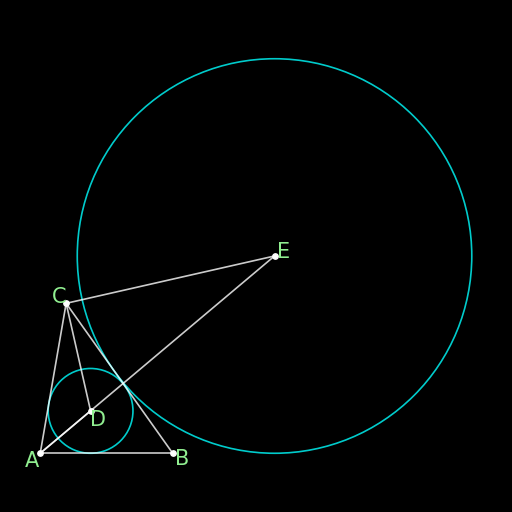
\includegraphics[width=0.55\textwidth]{figures/inbisector_exbisector.png}
\caption{Triangle $ABC$ with incenter $D$ and excenter $E$ (opposite $A$),
drawn by \texttt{numericals.py}. $CD$ is the internal bisector of
$\angle ACB$; $CE$ is the external bisector. The claim is $CD \perp CE$.}
\label{fig: inbisector-exbisector}
\end{figure}

\examplepart{Setting up the table}
Rather than running full DD+AR, the test
builds a bare \verb|AngleTable| directly and feeds it three facts by hand,
written using the directions $d(AC)$, $d(CD)$, $d(BC)$, $d(CE)$ from
\Cref{sec: d(AB)}:
\begin{itemize}
    \item \emph{fact1}: $CD$ bisects $\angle ACB$, i.e. the angle from $AC$ to
          $CD$ equals the angle from $CD$ to $BC$.
    \item \emph{fact2}: $CE$ is the external bisector of $\angle ACB$.
    \item \emph{fact3} (a distractor, deliberately unrelated to the
          perpendicularity claim): some other equal-angle fact about line
          $AB$, added only to confirm that AR's traceback correctly ignores
          it.
\end{itemize}

\examplepart{Watching the elimination happen, one fact at a time}
This is the
same incremental Gaussian elimination described above, but now traced
through concretely. Before any facts are added, the table only knows about
the constant:
\begin{lstlisting}
v2e:  pi = pi
\end{lstlisting}
After \emph{fact1} alone, $d(AC)$ is no longer free: the table has pivoted
and re-expressed it in terms of $d(BC)$ and $d(CD)$, which remain free
because nothing yet constrains them relative to each other:
\begin{lstlisting}
v2e:  d(ac) = -d(bc) + 2*d(cd)
      d(bc) = d(bc)
      d(cd) = d(cd)
      pi    = pi
\end{lstlisting}
This already says something: $d(AC) = 2d(CD) - d(BC)$, i.e.
$d(CD) = \tfrac12(d(AC)+d(BC))$ - a bisector's direction really is the
average of the two directions it bisects, and the table now carries that
fact for every later computation involving $d(AC)$. After \emph{fact2} is
also added, $d(CE)$ becomes expressible too, this time in terms of $d(CD)$
alone plus a multiple of $\pi$:
\begin{lstlisting}
v2e:  d(ac) = -d(bc) + 2*d(cd)
      d(bc) = d(bc)
      d(cd) = d(cd)
      d(ce) = d(cd) + -1/2*pi
      pi    = pi
\end{lstlisting}
This is already the answer, sitting in the table after only two facts: $d(CE)$
and $d(CD)$ differ by the constant $-\frac12\pi$. Adding the distractor
\emph{fact3} pivots $d(AB)$ into the table as well, but - this is the point
of including it - it does not touch the already-settled rows for $d(CD)$ or
$d(CE)$ at all:
\begin{lstlisting}
AR Table AngleTable (const=pi)
variables=6 eqs=12 groups=0
v2e (variable expansions):
  d(ab) = 3*d(bc) + -2*d(cd) + -pi
  d(ac) = -d(bc) + 2*d(cd)
  d(bc) = d(bc)
  d(cd) = d(cd)
  d(ce) = d(cd) + -1/2*pi
  pi = pi
\end{lstlisting}
The same final state, displayed as an explicit matrix (rows = every
direction seen so far, columns = the three basis quantities the system has
settled on - the constant \verb|pi|, and the two directions \verb|d(bc)| and
\verb|d(cd)| that turned out to be independent of everything else):
\begin{lstlisting}
var       pi        d(bc)     d(cd)
----------------------------------------
d(ab)     -1/1      3/1       -2/1
d(ac)     .         -1/1      2/1
d(bc)     .         1/1       .
d(cd)     .         .         1/1
d(ce)     -1/2      .         1/1
pi        1/1       .         .
\end{lstlisting}
Every row is to be read as "(row variable) = (entry under \texttt{pi})$\cdot
\pi$ + (entry under \texttt{d(bc)})$\cdot d(bc)$ + (entry under
\texttt{d(cd)})$\cdot d(cd)$", a dot meaning a zero coefficient; e.g. the
\verb|d(ce)| row reads $d(CE) = -\frac12 \pi + d(CD)$, matching the
\verb|v2e| line above it. Comparing the rows for \verb|d(cd)| and
\verb|d(ce)|: their difference is $d(CD) - d(CE) = \frac12\pi$, a
\emph{constant}, independent of the two remaining free variables
\verb|d(bc)|, \verb|d(cd)| - whatever the actual triangle looks like, this
difference never changes. A constant difference of exactly $\pi/2$ between
two directions is precisely what it means for two lines to be perpendicular,
so AR has discovered $CD \perp CE$ purely by linear algebra, without ever
consulting a rule about bisectors.

\examplepart{Finding out \emph{why}}
The table above answers \emph{whether} a
fact is true, but proof output also needs to know \emph{which} of the
original input facts were actually responsible - exactly the role
\verb|Dependency| objects play for DD in \Cref{sec: dd.py}. AR answers this
with a second matrix, completely separate from \verb|v2e|, by solving a
small linear program over it. \Cref{sec: AR LP} works through exactly how
this matrix is built and solved, first on a simple non-geometric example and
then on this very problem.

\subsection{Optional: Linear Programming and the \emph{Why} Matrix}\label{sec: AR LP}

\begin{lecturebox}{Optional deep dive}
This subsection first introduces linear programming as a mathematical topic
in its own right. Only after that do we return to AR and explain why a linear
program appears in proof traceback.
\end{lecturebox}

\examplepart{What is a linear program?}
A \emph{linear program} is an optimization problem in which both the
quantity being optimized and the constraints are linear. In one common
form, we choose a vector \(x=(x_1,\ldots,x_n)\in \mathbb{R}^n\) and solve
\[
\begin{array}{ll}
\text{minimize}   & c^\top x \\[2mm]
\text{subject to} & Ax \leq b,\\
                  & x\geq 0.
\end{array}
\]
The vector \(c\) gives the linear objective function, the inequalities
\(Ax\leq b\) describe the feasible region, and the condition \(x\geq0\)
usually means that the variables represent amounts of something: bags,
hours, weights, probabilities, or, later, weights assigned to proof facts.

Geometrically, the feasible region is an intersection of half-spaces, hence
a convex polygon in two variables, a convex polyhedron in three variables,
and a convex polytope in higher dimensions (possibly unbounded). The key
feature is that a linear objective has no hidden curvature. If an optimum
exists, one can find an optimum at a vertex of the feasible region.

\examplepart{Equality form}
The version used by \verb|scipy.optimize.linprog| in \verb|ar.py| is closer
to
\[
\begin{array}{ll}
\text{minimize}   & c^\top x \\[2mm]
\text{subject to} & A_{\mathrm{eq}}x=b_{\mathrm{eq}},\\
                  & x\geq0.
\end{array}
\]
This is called an \emph{equality-constrained} or \emph{standard-form}
linear program. Inequalities can be converted into equalities by adding
slack or surplus variables. For example, \(2p+q\geq5\) is equivalent to
\[
2p+q-s=5,\qquad s\geq0,
\]
where \(s\) records the amount by which the left-hand side exceeds the
minimum requirement.

\examplepart{A farmer example}
A farmer can buy two fertilizer mixes:
\[
\begin{array}{c|cc|c}
       & \text{nitrogen} & \text{phosphorus} & \text{cost} \\
\hline
P      & 2              & 1                 & 3 \\
Q      & 1              & 3                 & 2
\end{array}
\]
The field needs at least \(5\) units of nitrogen and at least \(5\) units of
phosphorus. If \(p,q\geq0\) are the numbers of bags of \(P\) and \(Q\), the
problem is
\[
\begin{array}{ll}
\text{minimize}   & 3p+2q \\[1mm]
\text{subject to} & 2p+q\geq5,\\
                  & p+3q\geq5,\\
                  & p,q\geq0.
\end{array}
\]
The two nutrient constraints meet at
\[
2p+q=5,\qquad p+3q=5,
\]
which gives \(p=2\), \(q=1\). The cost is \(3\cdot2+2\cdot1=8\).

Why is this optimal? The feasible region lies above both lines
\(2p+q=5\) and \(p+3q=5\) in the first quadrant. Moving the objective line
\(3p+2q=\text{constant}\) downward, the first feasible point it touches is
the intersection \((2,1)\). Other vertices are more expensive: using only
\(P\) requires \(p=5\), cost \(15\); using only \(Q\) requires \(q=5\), cost
\(10\). Thus the best solution is two bags of \(P\) and one bag of \(Q\).

A third mix \(R\) containing only potassium and sulfur would receive weight
\(0\) in an optimal solution, because it helps none of the two constraints
we care about while increasing the cost. This simple observation is the
part that will matter for AR: a linear program can automatically ignore
irrelevant ingredients.

\examplepart{Returning to AR}
In AR, the "ingredients" are not bags of fertilizer but previously known
linear facts. The target is not a nutrient requirement but a new equality
whose proof we want to explain. The question becomes:
\[
\text{Can the target equality be obtained as a linear combination of the
already registered facts?}
\]
This question is exactly an equality-form linear program. The matrix
\verb|self.A| stores the registered facts as columns. The vector
\verb|b_eq| stores the target equality we want to reproduce. Solving
\[
A_{\mathrm{eq}}x=b_{\mathrm{eq}}, \qquad x\geq0
\]
tells AR which facts were actually needed.

There is one technical wrinkle. In ordinary linear algebra one may combine
equations with positive or negative coefficients, but \verb|linprog| uses
non-negative variables. Therefore \verb|Table.register| stores two columns
per fact: one for using the fact forward and one for using it backward. The
signed coefficient is the difference between those two non-negative
weights.

\examplepart{Back to the bisector example}
For the worked example above, the registered facts give the following matrix:
\begin{lstlisting}
       fact1+  fact1-  fact2+  fact2-  fact3+  fact3-
d(ac)  [ 1      -1      -1       1      1      -1   ]
d(cd)  [-2       2       0       0      0       0   ]
d(bc)  [ 1      -1      -1       1     -2       2   ]
pi     [ 0       0       1      -1      1      -1   ]
d(ce)  [ 0       0       2      -2      0       0   ]
d(ab)  [ 0       0       0       0      1      -1   ]
\end{lstlisting}
Asking \emph{why} \(d(CD)-d(CE)=\tfrac12\pi\) produces a target vector with
\(+1\) on \verb|d(cd)|, \(-1\) on \verb|d(ce)|, and \(-\tfrac12\) on
\verb|pi|. Solving the equality-form LP gives:
\begin{lstlisting}
x* = (0, 0.5, 0, 0.5, 0, 0)      objective = -1
\end{lstlisting}
Thus \emph{fact1} and \emph{fact2} are used, each in the backward direction
with weight \(1/2\), while the distractor \emph{fact3} receives weight
\(0\). This is the AR analogue of the farmer's irrelevant mix \(R\): it is
available, but it is not needed to produce the target. The proof traceback
therefore reports exactly \texttt{['fact1', 'fact2']}.

\subsection{A Closer Look at the Language Model}\label{sec: lm.py}

DD and AR are sound and exhaustive, but they cannot invent a new point.
When both get stuck, the LM proposes one - a \emph{rabbit}
(\Cref{sec: Intro}) - which DD+AR then tries again. Two things make this
work with a model as small as $150$M parameters: how its training data was
generated, and how little it is actually asked to do at inference time.

\textbf{How one can make the training data.} The original paper
\cite{trinh2024solving} describes the central idea: avoid human-written
proof demonstrations by manufacturing many synthetic geometry problems.
For our purposes, the important point is not the exact engineering setup
used by DeepMind, but the mathematical recipe it suggests. The whole
pipeline can be read as a way of turning solved random diagrams into
supervised examples for auxiliary-point prediction.

The recipe is roughly this:
\begin{enumerate}
    \item \textbf{Generate a random construction.} Start from a small set of
          free points, then repeatedly apply construction rules such as
          ``take an intersection,'' ``draw a midpoint,'' ``construct an
          incenter,'' or ``put a point on a line.'' In code, these are the
          same kinds of actions listed in \verb|defs.txt|.
    \item \textbf{Close the diagram under DD+AR.} Treat the generated
          construction as a problem state and run the symbolic engine until
          saturation. The result is a large collection of true consequences:
          collinearities, equal angles, congruent segments, parallel lines,
          perpendicular lines, and so on.
    \item \textbf{Pick a derived fact as a theorem.} Any nontrivial derived
          fact can become the goal of a synthetic problem. For instance, if
          DD+AR derives \verb|perp C D C E|, we may ask a future solver to
          prove exactly that statement.
    \item \textbf{Trace the proof backwards.} Use the proof dependencies to
          find which earlier facts and which constructed points were actually
          needed. This is where \verb|trace_back.py| enters: it cuts away
          irrelevant parts of the random diagram and keeps a smaller proof
          core.
    \item \textbf{Hide one auxiliary point.} Compare the points needed to
          \emph{state} the theorem with the points needed in the proof. A
          point used in the proof but absent from the statement is precisely
          the kind of auxiliary point that human solvers often invent. Remove
          that construction from the visible problem, and use it as the
          target output for the language model.
\end{enumerate}

In slogan form: random construction creates a large true diagram; DD+AR
discovers many theorems inside it; traceback extracts a small proof; hiding
one proof-only point turns the theorem into a rabbit-prediction training
example. The paper reports doing this at very large scale: about one billion
random diagrams, reduced by proof search and deduplication to roughly
\(100\) million unique examples, of which about \(9\) million needed at least
one auxiliary point.

\begin{lecturebox}{What we will try to rebuild}
For our own basic AlphaGeometry-style system, we do not need the full
industrial-scale pipeline. We need a small version with the same logical
shape: generate random construction sequences, run DD+AR, select derived
goals, trace dependencies, detect proof-only points, and serialize examples
of the form ``problem state \(\mapsto\) useful auxiliary construction.'' This
will give us a local synthetic dataset we understand from end to end.
\end{lecturebox}

\textbf{What we can verify directly.} The checkpoint and its config are
public, and we confirmed the following ourselves while writing these notes
(by independently converting Google's released weights and loading the
result): a $12$-layer decoder-only transformer, embedding dimension $1024$,
$8$ heads, T5-style relative-position attention, about $152$M parameters,
and a vocabulary of under $1024$ tokens - DSL symbols only, never natural
language. Both the input (current stuck state) and output (proposed
construction) are the same compact token format seen throughout these notes,
e.g. \verb|e : C a c e 02 C b d e 03 ;| for
\verb|e = on_line e a c, on_line e b d|. At inference, \verb|lm_inference.py|
just runs beam search over this tiny vocabulary and returns a handful of
scored candidates - \Cref{sec: Running on Windows} showed this loop end to
end.

\textbf{What we will need to choose ourselves.} The public materials give
enough information to understand the idea, but not every engineering choice
needed to recreate the corpus. For our regeneration effort, we must choose:
how to sample random constructions, how large each diagram should be, which
derived facts count as interesting goals, how aggressively to deduplicate
near-identical examples, and how to format the final input-output strings.
Those choices are not a weakness of the project; they are exactly where a
course version can stay small, transparent, and mathematically inspectable.

\subsection{A Closer Look at \texttt{graph.py}}\label{sec: graph.py}

Every fact and table used so far has to live somewhere between calls to
\texttt{dd.py} and \texttt{ar.py}. That somewhere is a single \texttt{Graph}
object, built once per problem and threaded through the entire solve: it
holds every point, line, and segment seen so far, the
\texttt{atable}/\texttt{rtable}/\texttt{dtable} from \Cref{sec: ar.py}, and a
\texttt{cache} dictionary for quick dependency lookups. DD and AR only ever
read from and write into this one object.

\textbf{Two different kinds of ``related''.} The proof graph distinguishes
two relationships that are easy to conflate:
\begin{itemize}
    \item \emph{Adjacency} (\texttt{edge\_graph}, queried via
          \texttt{neighbors()}): a genuine structural link, e.g. ``point $P$
          lies on line $\ell$.'' This is the actual geometric picture.
    \item \emph{Equivalence} (\texttt{merge\_graph}, queried via
          \texttt{rep()}): a record that two nodes have been \emph{proven
          equal} - two lines turning out to be the same line, or two lengths
          turning out to be the same length. This has nothing to do with
          adjacency.
\end{itemize}
Equivalence is maintained as a union-find structure, documented directly in
\texttt{geometry.py}'s \texttt{Node} class:
\begin{lstlisting}
  a -> b -
          \
       c -> d -> e -> f -> g

d.merged_to = e
d.rep = g
d.merged_from = {a, b, c, d}
d.equivs = {a, b, c, d, e, f, g}
\end{lstlisting}
\texttt{rep()} just walks the chain of \texttt{rep\_by} pointers to the
representative; two nodes count as ``the same'' exactly when they share one.

\textbf{Where $d(\cdot)$ and $l(\cdot)$ actually come from.}
\Cref{sec: d(AB)} and \Cref{sec: ar.py} both used $d(AB)$ as notation for
line $AB$'s direction. It is not just notation - \texttt{connect\_val} builds
that exact string:
\begin{lstlisting}[style=pythonstyle]
def connect_val(self, node, deps):
    if node._val:
        return node._val
    name = None
    if isinstance(node, Line):
        name = 'd(' + node.name + ')'
    if isinstance(node, Angle):
        name = 'm(' + node.name + ')'
    if isinstance(node, Segment):
        name = 'l(' + node.name + ')'
    if isinstance(node, Ratio):
        name = 'r(' + node.name + ')'
    v = self.new_node(gm.val_type(node), name)
    self.connect(node, v, deps=deps)
    return v
\end{lstlisting}
Every \texttt{Line}, \texttt{Segment}, \texttt{Angle}, and \texttt{Ratio}
node has a separate \emph{value node} - its direction, length, measure, or
ratio - reachable as \texttt{node.\_val}. The geometric object and its value
are deliberately kept apart, because two different segments can share a
length without being the same segment.

\textbf{Why \texttt{cong} merges lengths, not segments.} This split is what
makes congruence work correctly. Proving $AB \cong CD$ calls:
\begin{lstlisting}[style=pythonstyle]
def make_equal(self, x, y, deps):
    self.connect_val(x, deps=None)
    self.connect_val(y, deps=None)
    vx, vy = x._val, y._val
    self.merge([vx, vy], deps)
\end{lstlisting}
which merges \texttt{x.\_val} and \texttt{y.\_val} - the two \emph{Length}
nodes - not \texttt{x} and \texttt{y} themselves. Afterwards $A,B,C,D$ are
still four distinct points and $AB$, $CD$ are still two distinct segments,
but \texttt{rep()} on their Length nodes now agrees, under a name like
\texttt{l(ab)}. Checking ``are $AB$ and $CD$ congruent?'' later is then a
single \texttt{rep()} comparison, however many other segments have
separately been proven equal to either one.

\bibliographystyle{alpha}
\bibliography{Ref}
\end{document}
